\documentclass[letterpaper]{book}
\usepackage{makeidx}
\usepackage{graphicx}
\usepackage{multicol}
\usepackage{float}
\usepackage{listings}
\usepackage{color}
\usepackage{ifthen}
\usepackage[table]{xcolor}
\usepackage{textcomp}
\usepackage{alltt}
\usepackage{ifpdf}
\ifpdf
\usepackage[pdftex,
            pagebackref=true,
            colorlinks=true,
            linkcolor=blue,
            unicode
           ]{hyperref}
\else
\usepackage[ps2pdf,
            pagebackref=true,
            colorlinks=true,
            linkcolor=blue,
            unicode
           ]{hyperref}
\usepackage{pspicture}
\fi
\usepackage[utf8]{inputenc}
\usepackage{mathptmx}
\usepackage[scaled=.90]{helvet}
\usepackage{courier}
\usepackage{doxygen}
\lstset{language=C++,inputencoding=utf8,basicstyle=\footnotesize,breaklines=true,breakatwhitespace=true,tabsize=8,numbers=left }
\makeindex
\setcounter{tocdepth}{3}
\renewcommand{\footrulewidth}{0.4pt}
\begin{document}
\hypersetup{pageanchor=false}
\begin{titlepage}
\vspace*{7cm}
\begin{center}
{\Large OneUp Wi-\/11 Simulator: Programmer's Guide }\\
\vspace*{1cm}
{\large Generated by Doxygen 1.7.2}\\
\vspace*{0.5cm}
{\small Mon Jan 24 2011 06:16:22}\\
\end{center}
\end{titlepage}
\clearemptydoublepage
\pagenumbering{roman}
\tableofcontents
\clearemptydoublepage
\pagenumbering{arabic}
\hypersetup{pageanchor=true}
\chapter{Introduction}
\label{index}\hypertarget{index}{}\hypertarget{index_intro}{}\section{Introduction}\label{index_intro}
The \char`\"{}Wi-\/11 Machine\char`\"{} is a simple, 16-\/bit computer architecture. It has 8 general purpose registers, 3 condition code registers (CCRs), and a program counter (PC). This software package is meant to emulate its execution, as well as present the user with information regarding the state of the machine after each instruction is executed. However, before one can delve into the behind-\/the-\/scenes details, one must understand the environment. In particular, an understanding of the object file syntax and the interactions between the components used in this project is necessary.\hypertarget{index_syntax}{}\section{Object Files}\label{index_syntax}
\begin{DoxyParagraph}{}
The object files (ususally file\_\-name.o) that this simulator accepts are ascii text files with the following structure: \begin{DoxyItemize}
\item One \hyperlink{index_header}{Header Record} \item Several \hyperlink{index_text}{Text Records} \item One \hyperlink{index_end}{End Record}\end{DoxyItemize}

\end{DoxyParagraph}
\hypertarget{index_header}{}\subsection{The Header Record}\label{index_header}
\begin{DoxyParagraph}{}
The Header Record is a single line that prepares the system for the storing the instructions to come. 
\end{DoxyParagraph}
\begin{DoxyParagraph}{}
{\bfseries Components} \begin{DoxyItemize}
\item A capital 'H'. This designates that it is the Header Record. \item A 6 character \char`\"{}segment name\char`\"{} (anything will do). \item A 4-\/digit Hexadecimal value that corresponds to the \char`\"{}load address\char`\"{} of the program. Instructions can be written starting at this address. \item A second 4-\/digit Hexadecimal value that denotes the length of the program-\/load segment (the size of memory into which the instructions will be loaded). \end{DoxyItemize}

\end{DoxyParagraph}
\begin{DoxyParagraph}{}
{\bfseries At a glance:} There is an 'H', a segment name, the first location where instructions can be written, and the number of memory locations for instuctions.
\end{DoxyParagraph}
\hypertarget{index_text}{}\subsection{Text Records}\label{index_text}
\begin{DoxyParagraph}{}
Following the Header Record are serveral Text Records. Each Text Record corresponds to a single machine instruction and, like the header record, is on a single line. 
\end{DoxyParagraph}
\begin{DoxyParagraph}{}
{\bfseries Components} \begin{DoxyItemize}
\item A capital 'T'. This designates that it is a Text Record. \item A 4-\/digit hexadecimal value -\/-\/ The location in memory at which the instruction will be stored. \item A second 4-\/digit Hexadecimal value -\/-\/ The encoding of the instruction to be stored. \end{DoxyItemize}

\end{DoxyParagraph}
\begin{DoxyParagraph}{}
{\bfseries At a glance:} There is a 'T', the location to store the instruction, and the instruction itself.
\end{DoxyParagraph}
\hypertarget{index_end}{}\subsection{The End Record}\label{index_end}
\begin{DoxyParagraph}{}
The End Record is, as the name would suggest, the last line of the line. Its purpose is to denote the end of instructions to be written and to give an initial value for the PC.\par
\par
 
\end{DoxyParagraph}
\begin{DoxyParagraph}{}
{\bfseries Components} \begin{DoxyItemize}
\item The End Record begins with a capital 'E'.\par
 \item Next, and last, a 4-\/digit hexadecimal value to be put into the PC. \end{DoxyItemize}

\end{DoxyParagraph}
\begin{DoxyParagraph}{}
{\bfseries At a glance:} There is an 'E', and the location in memory from which the first instruction should be fetched.
\end{DoxyParagraph}
\hypertarget{index_Component}{}\section{Interaction}\label{index_Component}

\begin{DoxyImageNoCaption}
  \mbox{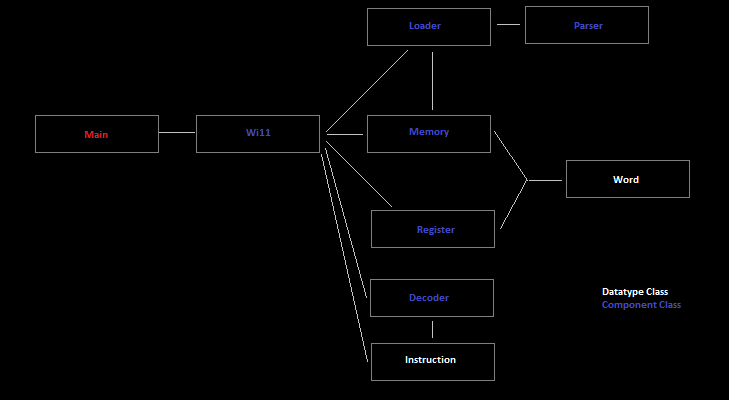
\includegraphics[width=\textwidth]{software_interaction.png}}
\end{DoxyImageNoCaption}
 \hypertarget{index_components}{}\subsection{Components}\label{index_components}
\hypertarget{index_instructions}{}\subsection{Wi11 Instruction Set}\label{index_instructions}

\chapter{Namespace Index}
\section{Namespace List}
Here is a list of all documented namespaces with brief descriptions:\begin{DoxyCompactList}
\item\contentsline{section}{\hyperlink{namespaceCodes}{Codes} (Values corresponding to the results of Wi-\/11 function calls )}{\pageref{namespaceCodes}}{}
\item\contentsline{section}{\hyperlink{namespaceDecoder__Directory}{Decoder\_\-Directory} (Declares register id's and instruction types for each register and instruction )}{\pageref{namespaceDecoder__Directory}}{}
\end{DoxyCompactList}

\chapter{Class Index}
\section{Class Hierarchy}
This inheritance list is sorted roughly, but not completely, alphabetically:\begin{DoxyCompactList}
\item \contentsline{section}{iInterpreter}{\pageref{classiInterpreter}}{}
\item \contentsline{section}{iMemory}{\pageref{classiMemory}}{}
\item \contentsline{section}{iRegister}{\pageref{classiRegister}}{}
\item \contentsline{section}{iSimulator}{\pageref{classiSimulator}}{}
\item \contentsline{section}{iWord}{\pageref{classiWord}}{}
\begin{DoxyCompactList}
\item \contentsline{section}{Word}{\pageref{classWord}}{}
\end{DoxyCompactList}
\item \contentsline{section}{Register}{\pageref{classRegister}}{}
\end{DoxyCompactList}

\chapter{Class Index}
\section{Class List}
Here are the classes, structs, unions and interfaces with brief descriptions:\begin{DoxyCompactList}
\item\contentsline{section}{\hyperlink{structWi11_1_1CCR}{Wi11::CCR} (Condition code registers: negative, zero, positive )}{\pageref{structWi11_1_1CCR}}{}
\item\contentsline{section}{\hyperlink{classiDecoder}{iDecoder} }{\pageref{classiDecoder}}{}
\item\contentsline{section}{\hyperlink{classiLoader}{iLoader} }{\pageref{classiLoader}}{}
\item\contentsline{section}{\hyperlink{classiMemory}{iMemory} (Mimics the functionality of memory in the Wi-\/11 machine )}{\pageref{classiMemory}}{}
\item\contentsline{section}{\hyperlink{structInstruction}{Instruction} }{\pageref{structInstruction}}{}
\item\contentsline{section}{\hyperlink{classiObjParser}{iObjParser} (Opens the object file and pre-\/processes each line )}{\pageref{classiObjParser}}{}
\item\contentsline{section}{\hyperlink{classiRegister}{iRegister} (Defines a \char`\"{}register\char`\"{} in the Wi-\/11 machine )}{\pageref{classiRegister}}{}
\item\contentsline{section}{\hyperlink{classiWi11}{iWi11} (Defines the internal logic of the Wi-\/11 )}{\pageref{classiWi11}}{}
\item\contentsline{section}{\hyperlink{classiWord}{iWord} (Defines a \char`\"{}word\char`\"{} of data on the Wi-\/11 Machine )}{\pageref{classiWord}}{}
\item\contentsline{section}{\hyperlink{classMemory}{Memory} }{\pageref{classMemory}}{}
\item\contentsline{section}{\hyperlink{structObjectData}{ObjectData} (A simple encoding of a \char`\"{}record\char`\"{} )}{\pageref{structObjectData}}{}
\item\contentsline{section}{\hyperlink{classRegister}{Register} }{\pageref{classRegister}}{}
\item\contentsline{section}{\hyperlink{classResultDecoder}{ResultDecoder} }{\pageref{classResultDecoder}}{}
\item\contentsline{section}{\hyperlink{classWi11}{Wi11} }{\pageref{classWi11}}{}
\item\contentsline{section}{\hyperlink{classWord}{Word} }{\pageref{classWord}}{}
\end{DoxyCompactList}

\chapter{File Index}
\section{File List}
Here is a list of all documented files with brief descriptions:\begin{DoxyCompactList}
\item\contentsline{section}{\hyperlink{iDecoder_8h}{iDecoder.h} (Definition of the Wi-\/11 instruction decoder )}{\pageref{iDecoder_8h}}{}
\item\contentsline{section}{\hyperlink{iLoader_8h}{iLoader.h} (Definition of the Wi-\/11 program loader )}{\pageref{iLoader_8h}}{}
\item\contentsline{section}{\hyperlink{iMemory_8h}{iMemory.h} (Definition of Wi-\/11 memory )}{\pageref{iMemory_8h}}{}
\item\contentsline{section}{\hyperlink{iObjParser_8h}{iObjParser.h} (Definition of the Object File Parser )}{\pageref{iObjParser_8h}}{}
\item\contentsline{section}{\hyperlink{iRegister_8h}{iRegister.h} (Definition of a \char`\"{}register\char`\"{} in the Wi-\/11 machine )}{\pageref{iRegister_8h}}{}
\item\contentsline{section}{\hyperlink{iWi11_8h}{iWi11.h} (Definition of the Wi-\/11 machine simulator )}{\pageref{iWi11_8h}}{}
\item\contentsline{section}{\hyperlink{iWord_8h}{iWord.h} (Definition of a \char`\"{}word\char`\"{} of data )}{\pageref{iWord_8h}}{}
\item\contentsline{section}{\hyperlink{Loader_8h}{Loader.h} (Definition of the private data for the \char`\"{}Loader\char`\"{} class )}{\pageref{Loader_8h}}{}
\item\contentsline{section}{\hyperlink{Memory_8h}{Memory.h} (Definition of private data for the \char`\"{}Memory\char`\"{} class )}{\pageref{Memory_8h}}{}
\item\contentsline{section}{\hyperlink{ObjParser_8cpp}{ObjParser.cpp} (Implements the declarations in \char`\"{}ObjParser.h\char`\"{} )}{\pageref{ObjParser_8cpp}}{}
\item\contentsline{section}{\hyperlink{ObjParser_8h}{ObjParser.h} (Definition of private data for the \char`\"{}ObjParser\char`\"{} class )}{\pageref{ObjParser_8h}}{}
\item\contentsline{section}{\hyperlink{Register_8h}{Register.h} (Definition of private data for the \char`\"{}Register\char`\"{} class )}{\pageref{Register_8h}}{}
\item\contentsline{section}{\hyperlink{ResultCodes_8h}{ResultCodes.h} (Definition of the Wi-\/11's run-\/time messages )}{\pageref{ResultCodes_8h}}{}
\item\contentsline{section}{\hyperlink{Wi11_8h}{Wi11.h} (Definition of the private data for the \char`\"{}Wi11\char`\"{} class )}{\pageref{Wi11_8h}}{}
\item\contentsline{section}{\hyperlink{Word_8cpp}{Word.cpp} (Implements the delcarations in \char`\"{}Word.h\char`\"{} )}{\pageref{Word_8cpp}}{}
\item\contentsline{section}{\hyperlink{Word_8h}{Word.h} (Definition of private data for the \char`\"{}Word\char`\"{} class )}{\pageref{Word_8h}}{}
\end{DoxyCompactList}

\chapter{Namespace Documentation}
\hypertarget{namespaceCodes}{
\section{Codes Namespace Reference}
\label{namespaceCodes}\index{Codes@{Codes}}
}


Values corresponding to the results of Wi-\/11 function calls.  


\subsection*{Enumerations}
\begin{DoxyCompactItemize}
\item 
enum {\bfseries RESULT} \{ \par
{\bfseries ERROR\_\-0}, 
{\bfseries SUCCESS}, 
{\bfseries HALT}, 
{\bfseries UNDEFINED}, 
\par
{\bfseries INVALID\_\-HEADER\_\-ENTRY}, 
{\bfseries INVALID\_\-DATA\_\-ENTRY}, 
{\bfseries OUT\_\-OF\_\-BOUNDS}, 
{\bfseries NOT\_\-HEX}, 
\par
{\bfseries FILE\_\-NOT\_\-FOUND}, 
{\bfseries INVALID\_\-TRAP\_\-CODE}
 \}
\end{DoxyCompactItemize}


\subsection{Detailed Description}
Values corresponding to the results of Wi-\/11 function calls. An enum is used for efficiency. The code can be returned up the collaboration hierarchy quickly so that, if necessary, the program can print an appropriate error message

\begin{DoxyNote}{Note}
\hyperlink{classResultDecoder}{ResultDecoder} can be used to do a look-\/up of the error message. 
\end{DoxyNote}

\hypertarget{namespaceDecoder__Directory}{
\section{Decoder\_\-Directory Namespace Reference}
\label{namespaceDecoder__Directory}\index{Decoder\_\-Directory@{Decoder\_\-Directory}}
}


Declares register id's and instruction types for each register and instruction.  


\subsection*{Enumerations}
\begin{DoxyCompactItemize}
\item 
enum {\bfseries REGISTER\_\-ID} \{ \par
{\bfseries R0}, 
{\bfseries R1}, 
{\bfseries R2}, 
{\bfseries R3}, 
\par
{\bfseries R4}, 
{\bfseries R5}, 
{\bfseries R6}, 
{\bfseries R7}, 
\par
{\bfseries PC}
 \}
\item 
enum {\bfseries INSTRUCTION\_\-TYPE} \{ \par
{\bfseries ADD}, 
{\bfseries AND}, 
{\bfseries BRx}, 
{\bfseries DBUG}, 
\par
{\bfseries JSR}, 
{\bfseries JSRR}, 
{\bfseries LD}, 
{\bfseries LDI}, 
\par
{\bfseries LDR}, 
{\bfseries LEA}, 
{\bfseries NOT}, 
{\bfseries RET}, 
\par
{\bfseries ST}, 
{\bfseries STI}, 
{\bfseries STR}, 
{\bfseries TRAP}, 
\par
{\bfseries ERROR}
 \}
\end{DoxyCompactItemize}


\subsection{Detailed Description}
Declares register id's and instruction types for each register and instruction. With these definitions, the process of executing instructions is made easier as REGISTER\_\-ID's and INSTRUCTION\_\-TYPE's can be used instead of strings. 
\chapter{Class Documentation}
\hypertarget{classDecoder}{
\section{Decoder Class Reference}
\label{classDecoder}\index{Decoder@{Decoder}}
}
\subsection*{Public Member Functions}
\begin{DoxyCompactItemize}
\item 
\hypertarget{classDecoder_a9f297296b2c7752b81f70acaeac1e732}{
\hyperlink{structInstruction}{Instruction} {\bfseries DecodeInstruction} (const \hyperlink{classiWord}{iWord} \&) const }
\label{classDecoder_a9f297296b2c7752b81f70acaeac1e732}

\end{DoxyCompactItemize}

\hypertarget{classiDecoder}{
\section{iDecoder Class Reference}
\label{classiDecoder}\index{iDecoder@{iDecoder}}
}


Defines how Wi-\/11 instructions are decoded.  


\subsection*{Public Member Functions}
\begin{DoxyCompactItemize}
\item 
virtual \hyperlink{structInstruction}{Instruction} \hyperlink{classiDecoder_a156d35f70da4bd96dce3b5b0b97d138c}{DecodeInstruction} (const \hyperlink{classiWord}{iWord} \&inst) const =0
\begin{DoxyCompactList}\small\item\em Translates the binary instruction into more usable objects. \item\end{DoxyCompactList}\end{DoxyCompactItemize}


\subsection{Detailed Description}
Defines how Wi-\/11 instructions are decoded. This could be a struct or even a function. It is declared as an object for consistency purposes. 

\subsection{Member Function Documentation}
\hypertarget{classiDecoder_a156d35f70da4bd96dce3b5b0b97d138c}{
\index{iDecoder@{iDecoder}!DecodeInstruction@{DecodeInstruction}}
\index{DecodeInstruction@{DecodeInstruction}!iDecoder@{iDecoder}}
\subsubsection[{DecodeInstruction}]{\setlength{\rightskip}{0pt plus 5cm}virtual {\bf Instruction} iDecoder::DecodeInstruction (
\begin{DoxyParamCaption}
\item[{const {\bf iWord} \&}]{ inst}
\end{DoxyParamCaption}
) const\hspace{0.3cm}{\ttfamily  \mbox{[}pure virtual\mbox{]}}}}
\label{classiDecoder_a156d35f70da4bd96dce3b5b0b97d138c}


Translates the binary instruction into more usable objects. 


\begin{DoxyParams}[1]{Parameters}
\mbox{\tt in}  & {\em inst} & The instruction to be translated. \\
\hline
\end{DoxyParams}
\begin{DoxyReturn}{Returns}
An \hyperlink{structInstruction}{Instruction} object as specified in \hyperlink{structInstruction}{its documentation}. 
\end{DoxyReturn}

\hypertarget{classiLoader}{
\section{iLoader Class Reference}
\label{classiLoader}\index{iLoader@{iLoader}}
}


Defines how the Wi-\/11 initializes memory.  




Inheritance diagram for iLoader:
\nopagebreak
\begin{figure}[H]
\begin{center}
\leavevmode
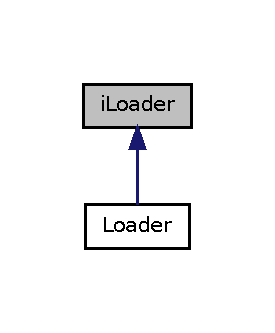
\includegraphics[width=132pt]{classiLoader__inherit__graph}
\end{center}
\end{figure}
\subsection*{Public Member Functions}
\begin{DoxyCompactItemize}
\item 
virtual \hyperlink{classiLoader_aeb68364c9e80d9dc5cb0f0299073c719}{iLoader} (\hyperlink{classiMemory}{iMemory} $\ast$mem)=0
\begin{DoxyCompactList}\small\item\em Set which \hyperlink{classMemory}{Memory} object is to be initialized by this object. \item\end{DoxyCompactList}\item 
virtual Codes::RESULT \hyperlink{classiLoader_a012bf942ef5210dd8797e1a20d8c5e13}{Load} (const char $\ast$filename, \hyperlink{classiWord}{iWord} \&PC\_\-address) const =0
\begin{DoxyCompactList}\small\item\em Perform the loads to memory (storing the instructions). \item\end{DoxyCompactList}\end{DoxyCompactItemize}


\subsection{Detailed Description}
Defines how the Wi-\/11 initializes memory. This class loads the instruction from the object file into memory. 

\subsection{Constructor \& Destructor Documentation}
\hypertarget{classiLoader_aeb68364c9e80d9dc5cb0f0299073c719}{
\index{iLoader@{iLoader}!iLoader@{iLoader}}
\index{iLoader@{iLoader}!iLoader@{iLoader}}
\subsubsection[{iLoader}]{\setlength{\rightskip}{0pt plus 5cm}iLoader::iLoader (
\begin{DoxyParamCaption}
\item[{{\bf iMemory} $\ast$}]{ mem}
\end{DoxyParamCaption}
)\hspace{0.3cm}{\ttfamily  \mbox{[}pure virtual\mbox{]}}}}
\label{classiLoader_aeb68364c9e80d9dc5cb0f0299073c719}


Set which \hyperlink{classMemory}{Memory} object is to be initialized by this object. 


\begin{DoxyParams}[1]{Parameters}
\mbox{\tt in}  & {\em mem} & The address where memory is located.\\
\hline
\end{DoxyParams}
\begin{DoxyNote}{Note}
Without this there would be nowhere to load the instructions. 
\end{DoxyNote}


Implemented in \hyperlink{classLoader_a337a13cc72c420d978660a2858ef8847}{Loader}.



\subsection{Member Function Documentation}
\hypertarget{classiLoader_a012bf942ef5210dd8797e1a20d8c5e13}{
\index{iLoader@{iLoader}!Load@{Load}}
\index{Load@{Load}!iLoader@{iLoader}}
\subsubsection[{Load}]{\setlength{\rightskip}{0pt plus 5cm}virtual Codes::RESULT iLoader::Load (
\begin{DoxyParamCaption}
\item[{const char $\ast$}]{ filename, }
\item[{{\bf iWord} \&}]{ PC\_\-address}
\end{DoxyParamCaption}
) const\hspace{0.3cm}{\ttfamily  \mbox{[}pure virtual\mbox{]}}}}
\label{classiLoader_a012bf942ef5210dd8797e1a20d8c5e13}


Perform the loads to memory (storing the instructions). 


\begin{DoxyParams}[1]{Parameters}
\mbox{\tt in}  & {\em filename} & The name of the object file to be read. \\
\hline
\mbox{\tt out}  & {\em PC\_\-address} & The value to be stored in the PC to start execution.  SUCCESS or, if something goes wrong, an appropriate error code.\\
\hline
\end{DoxyParams}
\begin{DoxyNote}{Note}
Multiple object files can be loaded using this, but the PC will be overwritten every time, so only the last End Record will matter (HOWEVER: the End Records still need to be present in each file). 
\end{DoxyNote}


Implemented in \hyperlink{classLoader_a134e26c9454ca019080aa9c06a4d52b4}{Loader}.


\hypertarget{classiMemory}{
\section{iMemory Class Reference}
\label{classiMemory}\index{iMemory@{iMemory}}
}


Defines the functionality of memory in the Wi-\/11 machine.  


\subsection*{Public Member Functions}
\begin{DoxyCompactItemize}
\item 
\hypertarget{classiMemory_aa9b57e00c0099963ab28489008d612e8}{
std::vector$<$ \hyperlink{classWord}{Word}\mbox{[}2\mbox{]}$>$ {\bfseries GetUsedMemory} () const =0}
\label{classiMemory_aa9b57e00c0099963ab28489008d612e8}

\item 
virtual \hyperlink{classWord}{Word} \hyperlink{classiMemory_a3352ba391fc9b69a0b8691b2d585596a}{Load} (const \hyperlink{classiWord}{iWord} \&w) const =0
\begin{DoxyCompactList}\small\item\em Performs a load. \item\end{DoxyCompactList}\item 
virtual Codes::RESULT \hyperlink{classiMemory_a27750e74d09fb473c163a4cc4c3e697b}{Reserve} (const \hyperlink{classiWord}{iWord} \&initial\_\-address, const \hyperlink{classiWord}{iWord} \&length)=0
\begin{DoxyCompactList}\small\item\em Reserves an initial section of memory for instructions. \item\end{DoxyCompactList}\item 
virtual Codes::RESULT \hyperlink{classiMemory_a2632c9999797b0799a7d6b0a59bfa91a}{Store} (const \hyperlink{classiWord}{iWord} \&address, const \hyperlink{classWord}{Word} \&value)=0
\begin{DoxyCompactList}\small\item\em Peforms a store. \item\end{DoxyCompactList}\end{DoxyCompactItemize}


\subsection{Detailed Description}
Defines the functionality of memory in the Wi-\/11 machine. Its size is limited only by addressability (2$^\wedge$16-\/1 16-\/bit words). It is meant to be implemented in such a way that the memory initialized for instructions can be accessed in constant time while addresses outside this range are accessed in nlogn time. 

\subsection{Member Function Documentation}
\hypertarget{classiMemory_a27750e74d09fb473c163a4cc4c3e697b}{
\index{iMemory@{iMemory}!Reserve@{Reserve}}
\index{Reserve@{Reserve}!iMemory@{iMemory}}
\subsubsection[{Reserve}]{\setlength{\rightskip}{0pt plus 5cm}virtual Codes::RESULT iMemory::Reserve (
\begin{DoxyParamCaption}
\item[{const {\bf iWord} \&}]{ initial\_\-address, }
\item[{const {\bf iWord} \&}]{ length}
\end{DoxyParamCaption}
)\hspace{0.3cm}{\ttfamily  \mbox{[}pure virtual\mbox{]}}}}
\label{classiMemory_a27750e74d09fb473c163a4cc4c3e697b}


Reserves an initial section of memory for instructions. 


\begin{DoxyParams}[1]{Parameters}
\mbox{\tt in}  & {\em initial\_\-address} & The smallest address for the instruction memory. \\
\hline
\mbox{\tt in}  & {\em length} & The number of addresses to reserve. \\
\hline
\end{DoxyParams}
\begin{DoxyReturn}{Returns}
SUCCESS or, if something goes wrong, an appropriate error code.
\end{DoxyReturn}
The memory reserved here is dynamically allocated and provides constant-\/time access to addresses \char`\"{}initial\_\-address\char`\"{} through \char`\"{}initial\_\-address\char`\"{}+\char`\"{}length\char`\"{}-\/1. \hypertarget{classiMemory_a3352ba391fc9b69a0b8691b2d585596a}{
\index{iMemory@{iMemory}!Load@{Load}}
\index{Load@{Load}!iMemory@{iMemory}}
\subsubsection[{Load}]{\setlength{\rightskip}{0pt plus 5cm}virtual {\bf Word} iMemory::Load (
\begin{DoxyParamCaption}
\item[{const {\bf iWord} \&}]{ w}
\end{DoxyParamCaption}
) const\hspace{0.3cm}{\ttfamily  \mbox{[}pure virtual\mbox{]}}}}
\label{classiMemory_a3352ba391fc9b69a0b8691b2d585596a}


Performs a load. 


\begin{DoxyParams}[1]{Parameters}
\mbox{\tt in}  & {\em w} & The address from which to load data. \\
\hline
\end{DoxyParams}
\begin{DoxyReturn}{Returns}
The data stored a address \char`\"{}w\char`\"{}.
\end{DoxyReturn}
\begin{DoxyNote}{Note}
If \char`\"{}w\char`\"{} is in the range created by Reserve(), it can be accessed in constant time. Otherwise, a maximum of nlogn time is required if n is the size of memory initialized outside of these boundaries. 
\end{DoxyNote}
\hypertarget{classiMemory_a2632c9999797b0799a7d6b0a59bfa91a}{
\index{iMemory@{iMemory}!Store@{Store}}
\index{Store@{Store}!iMemory@{iMemory}}
\subsubsection[{Store}]{\setlength{\rightskip}{0pt plus 5cm}virtual Codes::RESULT iMemory::Store (
\begin{DoxyParamCaption}
\item[{const {\bf iWord} \&}]{ address, }
\item[{const {\bf Word} \&}]{ value}
\end{DoxyParamCaption}
)\hspace{0.3cm}{\ttfamily  \mbox{[}pure virtual\mbox{]}}}}
\label{classiMemory_a2632c9999797b0799a7d6b0a59bfa91a}


Peforms a store. 


\begin{DoxyParams}[1]{Parameters}
\mbox{\tt in}  & {\em address} & The address to store the data. \\
\hline
\mbox{\tt in}  & {\em value} & The data to store at \char`\"{}address\char`\"{}. \\
\hline
\end{DoxyParams}
\begin{DoxyReturn}{Returns}
SUCCESS or, if something went wrong, an appropriate error code.
\end{DoxyReturn}
\begin{DoxyNote}{Note}
The efficiency constraints in Load() apply here as well. 
\end{DoxyNote}

\hypertarget{structInstruction}{
\section{Instruction Struct Reference}
\label{structInstruction}\index{Instruction@{Instruction}}
}


Container to simplify interactions with Wi-\/11 instructions.  


\subsection*{Public Attributes}
\begin{DoxyCompactItemize}
\item 
\hypertarget{structInstruction_afc9f26527635d9d851759eab142e5ec7}{
INSTRUCTION\_\-TYPE \hyperlink{structInstruction_afc9f26527635d9d851759eab142e5ec7}{type}}
\label{structInstruction_afc9f26527635d9d851759eab142e5ec7}

\begin{DoxyCompactList}\small\item\em The type of instruction. \item\end{DoxyCompactList}\item 
std::vector$<$ \hyperlink{classWord}{Word} $>$ \hyperlink{structInstruction_a93f6b7366b14b17d8379ea952687960c}{data}
\begin{DoxyCompactList}\small\item\em The arguemnts to the operation (including unecessary bits). \item\end{DoxyCompactList}\end{DoxyCompactItemize}


\subsection{Detailed Description}
Container to simplify interactions with Wi-\/11 instructions. 

\subsection{Member Data Documentation}
\hypertarget{structInstruction_a93f6b7366b14b17d8379ea952687960c}{
\index{Instruction@{Instruction}!data@{data}}
\index{data@{data}!Instruction@{Instruction}}
\subsubsection[{data}]{\setlength{\rightskip}{0pt plus 5cm}std::vector$<${\bf Word}$>$ {\bf Instruction::data}}}
\label{structInstruction_a93f6b7366b14b17d8379ea952687960c}


The arguemnts to the operation (including unecessary bits). 

\begin{DoxyParagraph}{Example:}
The add instruction comes in two forms: 
\end{DoxyParagraph}
\begin{DoxyParagraph}{}
\begin{DoxyItemize}
\item dest\_\-reg = source\_\-reg\_\-1 + source\_\-reg\_\-2 For this form, the encoding (as ordered) is as follows: 
\begin{DoxyItemize}
\item dest\_\-reg 
\item source\_\-reg\_\-1 
\item a 0 
\item 2 unused bits 
\item source\_\-reg\_\-2 These segments are each an element of the data vector. 
\end{DoxyItemize}\end{DoxyItemize}

\end{DoxyParagraph}
\begin{DoxyParagraph}{}
\begin{DoxyItemize}
\item dest\_\-reg = source\_\-reg + immediate\_\-value For this form, the encoding (as ordered) is as follows: 
\begin{DoxyItemize}
\item op code 
\item dest\_\-reg 
\item source\_\-reg\_\-1 
\item a 1 
\item a 5-\/bit immediate value These segments are also each an element of the data vector. 
\end{DoxyItemize}In short, any division specified in \hyperlink{index_instructions}{Wi11 Instruction Set} will be an element of the data vector.\end{DoxyItemize}

\end{DoxyParagraph}
\begin{DoxyNote}{Note}
Both of the overloaded instructions (ADD and AND) can be differentiated by the number of divisions: \begin{DoxyItemize}
\item ADD with two registers has 5 \item ADD with a register and immediate has 4 and \item AND with two registers has 5 \item AND with a register and immediate has 4 Thus the fifth bit (either a 1 or 0) is not needed to determine the variation of the instruction (HOWEVER: the 1 or 0 is still included). \end{DoxyItemize}

\end{DoxyNote}

\hypertarget{classiObjParser}{
\section{iObjParser Class Reference}
\label{classiObjParser}\index{iObjParser@{iObjParser}}
}


Opens the object file and pre-\/processes each line.  


\subsection*{Public Member Functions}
\begin{DoxyCompactItemize}
\item 
\hypertarget{classiObjParser_ae88aacaa19a6aa6d4a7c82c02eabc3dc}{
virtual \hyperlink{classiObjParser_ae88aacaa19a6aa6d4a7c82c02eabc3dc}{$\sim$iObjParser} ()=0}
\label{classiObjParser_ae88aacaa19a6aa6d4a7c82c02eabc3dc}

\begin{DoxyCompactList}\small\item\em Closes a file, if necessarily, when an \hyperlink{classiObjParser}{iObjParser} object goes out of scope.. \item\end{DoxyCompactList}\item 
virtual Codes::Result \hyperlink{classiObjParser_a570e7a7dfb64b66e7a78f75ec4da193a}{Initialize} (const char $\ast$filename)=0
\begin{DoxyCompactList}\small\item\em Attempts to open th object file. \item\end{DoxyCompactList}\item 
virtual \hyperlink{structObjectData}{ObjectData} \hyperlink{classiObjParser_aeb9af4a40a06e755d8b0e493526d82dd}{GetNext} ()=0
\begin{DoxyCompactList}\small\item\em Pre-\/processes the next line of the object file. \item\end{DoxyCompactList}\end{DoxyCompactItemize}


\subsection{Detailed Description}
Opens the object file and pre-\/processes each line. 

\subsection{Member Function Documentation}
\hypertarget{classiObjParser_a570e7a7dfb64b66e7a78f75ec4da193a}{
\index{iObjParser@{iObjParser}!Initialize@{Initialize}}
\index{Initialize@{Initialize}!iObjParser@{iObjParser}}
\subsubsection[{Initialize}]{\setlength{\rightskip}{0pt plus 5cm}virtual Codes::Result iObjParser::Initialize (
\begin{DoxyParamCaption}
\item[{const char $\ast$}]{ filename}
\end{DoxyParamCaption}
)\hspace{0.3cm}{\ttfamily  \mbox{[}pure virtual\mbox{]}}}}
\label{classiObjParser_a570e7a7dfb64b66e7a78f75ec4da193a}


Attempts to open th object file. 


\begin{DoxyParams}[1]{Parameters}
\mbox{\tt in}  & {\em filename} & The name of the object file to be opened. \\
\hline
\end{DoxyParams}
\begin{DoxyReturn}{Returns}
SUCCESS or, if something went wrong, an appropriate error code.
\end{DoxyReturn}
If another file is open, closes that file first before attempting to open the new one. \hypertarget{classiObjParser_aeb9af4a40a06e755d8b0e493526d82dd}{
\index{iObjParser@{iObjParser}!GetNext@{GetNext}}
\index{GetNext@{GetNext}!iObjParser@{iObjParser}}
\subsubsection[{GetNext}]{\setlength{\rightskip}{0pt plus 5cm}virtual {\bf ObjectData} iObjParser::GetNext (
\begin{DoxyParamCaption}
{}
\end{DoxyParamCaption}
)\hspace{0.3cm}{\ttfamily  \mbox{[}pure virtual\mbox{]}}}}
\label{classiObjParser_aeb9af4a40a06e755d8b0e493526d82dd}


Pre-\/processes the next line of the object file. 

\begin{DoxyPrecond}{Precondition}
Initialize must have successfully opened a file. 
\end{DoxyPrecond}
\begin{DoxyReturn}{Returns}
The encoding of the next instruction.
\end{DoxyReturn}
If there is an error parsing the entry: \begin{DoxyItemize}
\item \hyperlink{structObjectData_a77f1a74deb864606b1b5cc115c2a99a5}{ObjectData.type} = 0; \item \hyperlink{structObjectData_af755ea276bafd67e377e869950c1eb48}{ObjectData.data} = \mbox{[}the faulty encoding\mbox{]} \end{DoxyItemize}

\hypertarget{classiRegister}{
\section{iRegister Class Reference}
\label{classiRegister}\index{iRegister@{iRegister}}
}


Defines a \char`\"{}register\char`\"{} in the Wi-\/11 machine.  




Inheritance diagram for iRegister:\nopagebreak
\begin{figure}[H]
\begin{center}
\leavevmode
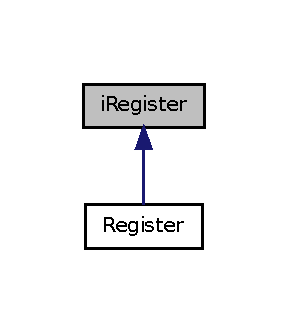
\includegraphics[width=136pt]{classiRegister__inherit__graph}
\end{center}
\end{figure}
\subsection*{Public Member Functions}
\begin{DoxyCompactItemize}
\item 
virtual \hyperlink{classWord}{Word} \hyperlink{classiRegister_ae7266f6f981b621f53f3c7cf77d4966a}{GetValue} () const =0
\begin{DoxyCompactList}\small\item\em Retrieves a copy of the word of data store in the register. \item\end{DoxyCompactList}\item 
virtual void \hyperlink{classiRegister_acb13aa880933f43088958723c9d6e564}{Add} (const \hyperlink{classiWord}{iWord} \&w)=0
\begin{DoxyCompactList}\small\item\em Adds a word of data to the calling object. \item\end{DoxyCompactList}\item 
virtual \hyperlink{classRegister}{Register} \hyperlink{classiRegister_abaaacfa8cb18bea90a78673bd572a1c8}{Add} (const \hyperlink{classiRegister}{iRegister} \&r) const =0
\begin{DoxyCompactList}\small\item\em Adds a word of data to the calling object. \item\end{DoxyCompactList}\item 
virtual \hyperlink{classRegister}{Register} \hyperlink{classiRegister_af8ab19234f44a0bade65cb35fd2cd036}{operator+} (const \hyperlink{classiRegister}{iRegister} \&r) const =0
\begin{DoxyCompactList}\small\item\em A standard add operator. \item\end{DoxyCompactList}\item 
virtual void \hyperlink{classiRegister_a98de346c2d0b15bee47d76bc5f70e94b}{Subtract} (const \hyperlink{classiWord}{iWord} \&w)=0
\begin{DoxyCompactList}\small\item\em Subtracts a word of data from the calling object. \item\end{DoxyCompactList}\item 
virtual \hyperlink{classRegister}{Register} \hyperlink{classiRegister_ad7eb424400d184f1829664dd4f87ce5c}{Subtract} (const \hyperlink{classiRegister}{iRegister} \&r) const =0
\begin{DoxyCompactList}\small\item\em Subtracts a word of data from the calling object. \item\end{DoxyCompactList}\item 
virtual \hyperlink{classRegister}{Register} \hyperlink{classiRegister_a01f837097cb87ec33fdc1cef606e1842}{operator-\/} (const \hyperlink{classiRegister}{iRegister} \&r) const =0
\begin{DoxyCompactList}\small\item\em A standard subtraction operator. \item\end{DoxyCompactList}\item 
virtual void \hyperlink{classiRegister_ae8114106e70653a705f04ba3892ed9e1}{And} (const \hyperlink{classiWord}{iWord} \&w)=0
\begin{DoxyCompactList}\small\item\em Performs a bit-\/wise and. \item\end{DoxyCompactList}\item 
virtual \hyperlink{classRegister}{Register} \hyperlink{classiRegister_aa9a15ebfeea1e5857a1098b73cc583ad}{And} (const \hyperlink{classiRegister}{iRegister} \&r) const =0
\begin{DoxyCompactList}\small\item\em Performs a bit-\/wise and. \item\end{DoxyCompactList}\item 
virtual void \hyperlink{classiRegister_aa0eac4fe58bde4a280a42fda1c087eee}{Or} (const \hyperlink{classiWord}{iWord} \&w)=0
\begin{DoxyCompactList}\small\item\em Performs a bit-\/wise \char`\"{}or\char`\"{}. \item\end{DoxyCompactList}\item 
virtual \hyperlink{classRegister}{Register} \hyperlink{classiRegister_af5f065e89ef31d2ed40a1e80d9231bfd}{Or} (const \hyperlink{classiRegister}{iRegister} \&r) const =0
\begin{DoxyCompactList}\small\item\em Performs a bit-\/wise or. \item\end{DoxyCompactList}\item 
virtual void \hyperlink{classiRegister_af4bbbe945b151dee3f1743c43a451cb3}{Not} ()=0
\begin{DoxyCompactList}\small\item\em Performs a bit-\/wise not. \item\end{DoxyCompactList}\item 
virtual \hyperlink{classRegister}{Register} \hyperlink{classiRegister_aca99e377de5cd1ef136a850d85143cf3}{Not} () const =0
\begin{DoxyCompactList}\small\item\em Performs a bit-\/wise not. \item\end{DoxyCompactList}\item 
virtual void \hyperlink{classiRegister_a8ffac24d1d7326e1a15f9b37cd426969}{Store} (const \hyperlink{classiWord}{iWord} \&w)=0
\begin{DoxyCompactList}\small\item\em Stores a word of data. \item\end{DoxyCompactList}\item 
virtual void \hyperlink{classiRegister_ac2b021b80a890f010fc68826e29fee47}{Store} (const \hyperlink{classiRegister}{iRegister} \&r)=0
\begin{DoxyCompactList}\small\item\em Stores a copy of another register. \item\end{DoxyCompactList}\item 
virtual \hyperlink{classRegister}{Register} \& \hyperlink{classiRegister_a16bf3f305a9588ddc85c109ac9a8b47b}{operator=} (const \hyperlink{classiWord}{iWord} \&w)=0
\begin{DoxyCompactList}\small\item\em A standard assignment operator. \item\end{DoxyCompactList}\item 
virtual \hyperlink{classRegister}{Register} \& \hyperlink{classiRegister_a3280dc5af6b828d875c57c3a3eac54d9}{operator=} (const \hyperlink{classRegister}{Register} r)=0
\begin{DoxyCompactList}\small\item\em A standard assignment operator. \item\end{DoxyCompactList}\item 
virtual \hyperlink{classRegister}{Register} \& \hyperlink{classiRegister_abca2bcea556d63fb4e3504df221cdc62}{operator++} ()=0
\begin{DoxyCompactList}\small\item\em A standard pre-\/increment operator. \item\end{DoxyCompactList}\item 
virtual \hyperlink{classRegister}{Register} \& \hyperlink{classiRegister_a36e6e1bfbc6a9fe203e8fb5b9f6396cb}{operator++} (int)=0
\begin{DoxyCompactList}\small\item\em A standard post-\/increment operator. \item\end{DoxyCompactList}\end{DoxyCompactItemize}


\subsection{Detailed Description}
Defines a \char`\"{}register\char`\"{} in the Wi-\/11 machine. The methods present in this inteface are meant to mimic the functionality of the Wi-\/11 machine, allowing for simplified execution of the instructions therein. This interace class will serve as a base from which the general purpose registers and program counter of the Wi-\/11 can be defined. 

\subsection{Member Function Documentation}
\hypertarget{classiRegister_ae7266f6f981b621f53f3c7cf77d4966a}{
\index{iRegister@{iRegister}!GetValue@{GetValue}}
\index{GetValue@{GetValue}!iRegister@{iRegister}}
\subsubsection[{GetValue}]{\setlength{\rightskip}{0pt plus 5cm}virtual {\bf Word} iRegister::GetValue (
\begin{DoxyParamCaption}
{}
\end{DoxyParamCaption}
) const\hspace{0.3cm}{\ttfamily  \mbox{[}pure virtual\mbox{]}}}}
\label{classiRegister_ae7266f6f981b621f53f3c7cf77d4966a}


Retrieves a copy of the word of data store in the register. 

\begin{DoxyPostcond}{Postcondition}
The value of the calling object is not changed. 
\end{DoxyPostcond}
\begin{DoxyReturn}{Returns}
A new \hyperlink{classWord}{Word} object holding the value that is stored in the register. 
\end{DoxyReturn}


Implemented in \hyperlink{classRegister_a379734c28ab8258ce528a96de24cfa1a}{Register}.

\hypertarget{classiRegister_acb13aa880933f43088958723c9d6e564}{
\index{iRegister@{iRegister}!Add@{Add}}
\index{Add@{Add}!iRegister@{iRegister}}
\subsubsection[{Add}]{\setlength{\rightskip}{0pt plus 5cm}virtual void iRegister::Add (
\begin{DoxyParamCaption}
\item[{const {\bf iWord} \&}]{ w}
\end{DoxyParamCaption}
)\hspace{0.3cm}{\ttfamily  \mbox{[}pure virtual\mbox{]}}}}
\label{classiRegister_acb13aa880933f43088958723c9d6e564}


Adds a word of data to the calling object. 


\begin{DoxyParams}[1]{Parameters}
\mbox{\tt in}  & {\em w} & The value to be added. \\
\hline
\end{DoxyParams}
\begin{DoxyPostcond}{Postcondition}
The calling object equals its previous value plus the value of \char`\"{}w\char`\"{}; \char`\"{}w\char`\"{}, however, will remain unchanged. 
\end{DoxyPostcond}


Implemented in \hyperlink{classRegister_a73d8564754d7ddb7e8349001010e688b}{Register}.

\hypertarget{classiRegister_abaaacfa8cb18bea90a78673bd572a1c8}{
\index{iRegister@{iRegister}!Add@{Add}}
\index{Add@{Add}!iRegister@{iRegister}}
\subsubsection[{Add}]{\setlength{\rightskip}{0pt plus 5cm}virtual {\bf Register} iRegister::Add (
\begin{DoxyParamCaption}
\item[{const {\bf iRegister} \&}]{ r}
\end{DoxyParamCaption}
) const\hspace{0.3cm}{\ttfamily  \mbox{[}pure virtual\mbox{]}}}}
\label{classiRegister_abaaacfa8cb18bea90a78673bd572a1c8}


Adds a word of data to the calling object. 


\begin{DoxyParams}[1]{Parameters}
\mbox{\tt in}  & {\em r} & The value to be added. \\
\hline
\end{DoxyParams}
\begin{DoxyPostcond}{Postcondition}
Both the calling object and \char`\"{}r\char`\"{} will not be changed. 
\end{DoxyPostcond}
\begin{DoxyReturn}{Returns}
A new \hyperlink{classRegister}{Register} object holding the value of the calling object plus the value in \char`\"{}r\char`\"{}. 
\end{DoxyReturn}


Implemented in \hyperlink{classRegister_a9d9c6801db55e8706eb242b1e0e0fa3f}{Register}.

\hypertarget{classiRegister_af8ab19234f44a0bade65cb35fd2cd036}{
\index{iRegister@{iRegister}!operator+@{operator+}}
\index{operator+@{operator+}!iRegister@{iRegister}}
\subsubsection[{operator+}]{\setlength{\rightskip}{0pt plus 5cm}virtual {\bf Register} iRegister::operator+ (
\begin{DoxyParamCaption}
\item[{const {\bf iRegister} \&}]{ r}
\end{DoxyParamCaption}
) const\hspace{0.3cm}{\ttfamily  \mbox{[}pure virtual\mbox{]}}}}
\label{classiRegister_af8ab19234f44a0bade65cb35fd2cd036}


A standard add operator. 

\begin{DoxyNote}{Note}
\char`\"{}result = p + r\char`\"{} is equivalent to \char`\"{}result = p.Add(r)\char`\"{}. 
\end{DoxyNote}


Implemented in \hyperlink{classRegister_a55de0c3b5f8fe14df7c24bce777204e0}{Register}.

\hypertarget{classiRegister_a98de346c2d0b15bee47d76bc5f70e94b}{
\index{iRegister@{iRegister}!Subtract@{Subtract}}
\index{Subtract@{Subtract}!iRegister@{iRegister}}
\subsubsection[{Subtract}]{\setlength{\rightskip}{0pt plus 5cm}virtual void iRegister::Subtract (
\begin{DoxyParamCaption}
\item[{const {\bf iWord} \&}]{ w}
\end{DoxyParamCaption}
)\hspace{0.3cm}{\ttfamily  \mbox{[}pure virtual\mbox{]}}}}
\label{classiRegister_a98de346c2d0b15bee47d76bc5f70e94b}


Subtracts a word of data from the calling object. 


\begin{DoxyParams}[1]{Parameters}
\mbox{\tt in}  & {\em w} & The value to be subtracted. \\
\hline
\end{DoxyParams}
\begin{DoxyPostcond}{Postcondition}
The calling object equals its previous value minus the value of \char`\"{}w\char`\"{}; \char`\"{}w\char`\"{}, however, will remain unchanged. 
\end{DoxyPostcond}


Implemented in \hyperlink{classRegister_a726a720b6bcca282945f1c0a65ca0dd4}{Register}.

\hypertarget{classiRegister_ad7eb424400d184f1829664dd4f87ce5c}{
\index{iRegister@{iRegister}!Subtract@{Subtract}}
\index{Subtract@{Subtract}!iRegister@{iRegister}}
\subsubsection[{Subtract}]{\setlength{\rightskip}{0pt plus 5cm}virtual {\bf Register} iRegister::Subtract (
\begin{DoxyParamCaption}
\item[{const {\bf iRegister} \&}]{ r}
\end{DoxyParamCaption}
) const\hspace{0.3cm}{\ttfamily  \mbox{[}pure virtual\mbox{]}}}}
\label{classiRegister_ad7eb424400d184f1829664dd4f87ce5c}


Subtracts a word of data from the calling object. 


\begin{DoxyParams}[1]{Parameters}
\mbox{\tt in}  & {\em r} & The value to be subtracted. \\
\hline
\end{DoxyParams}
\begin{DoxyPostcond}{Postcondition}
Both the calling object and \char`\"{}r\char`\"{} will not be changed. 
\end{DoxyPostcond}
\begin{DoxyReturn}{Returns}
A new \hyperlink{classRegister}{Register} object holding the value of the calling object minus the value in \char`\"{}r\char`\"{}. 
\end{DoxyReturn}


Implemented in \hyperlink{classRegister_a05132a4a62f5c6883fdf78731970ab6a}{Register}.

\hypertarget{classiRegister_a01f837097cb87ec33fdc1cef606e1842}{
\index{iRegister@{iRegister}!operator-\/@{operator-\/}}
\index{operator-\/@{operator-\/}!iRegister@{iRegister}}
\subsubsection[{operator-\/}]{\setlength{\rightskip}{0pt plus 5cm}virtual {\bf Register} iRegister::operator-\/ (
\begin{DoxyParamCaption}
\item[{const {\bf iRegister} \&}]{ r}
\end{DoxyParamCaption}
) const\hspace{0.3cm}{\ttfamily  \mbox{[}pure virtual\mbox{]}}}}
\label{classiRegister_a01f837097cb87ec33fdc1cef606e1842}


A standard subtraction operator. 

\begin{DoxyNote}{Note}
\char`\"{}result = p -\/ r\char`\"{} is equivalent to \char`\"{}result = r.Subtract(w)\char`\"{}. 
\end{DoxyNote}


Implemented in \hyperlink{classRegister_a43c957e4b6a3103f0634258891c82b46}{Register}.

\hypertarget{classiRegister_ae8114106e70653a705f04ba3892ed9e1}{
\index{iRegister@{iRegister}!And@{And}}
\index{And@{And}!iRegister@{iRegister}}
\subsubsection[{And}]{\setlength{\rightskip}{0pt plus 5cm}virtual void iRegister::And (
\begin{DoxyParamCaption}
\item[{const {\bf iWord} \&}]{ w}
\end{DoxyParamCaption}
)\hspace{0.3cm}{\ttfamily  \mbox{[}pure virtual\mbox{]}}}}
\label{classiRegister_ae8114106e70653a705f04ba3892ed9e1}


Performs a bit-\/wise and. 


\begin{DoxyParams}[1]{Parameters}
\mbox{\tt in}  & {\em w} & The value to be \char`\"{}and\char`\"{}ed. \\
\hline
\end{DoxyParams}
\begin{DoxyPostcond}{Postcondition}
The calling object equals its previous value bit-\/wise and'ed with w. 
\end{DoxyPostcond}


Implemented in \hyperlink{classRegister_a312263efb06ef459409879f5119b3b81}{Register}.

\hypertarget{classiRegister_aa9a15ebfeea1e5857a1098b73cc583ad}{
\index{iRegister@{iRegister}!And@{And}}
\index{And@{And}!iRegister@{iRegister}}
\subsubsection[{And}]{\setlength{\rightskip}{0pt plus 5cm}virtual {\bf Register} iRegister::And (
\begin{DoxyParamCaption}
\item[{const {\bf iRegister} \&}]{ r}
\end{DoxyParamCaption}
) const\hspace{0.3cm}{\ttfamily  \mbox{[}pure virtual\mbox{]}}}}
\label{classiRegister_aa9a15ebfeea1e5857a1098b73cc583ad}


Performs a bit-\/wise and. 


\begin{DoxyParams}[1]{Parameters}
\mbox{\tt in}  & {\em r} & The value to be \char`\"{}and\char`\"{}ed. \\
\hline
\end{DoxyParams}
\begin{DoxyPostcond}{Postcondition}
Both the calling object and r are not changed. 
\end{DoxyPostcond}
\begin{DoxyReturn}{Returns}
A new \hyperlink{classRegister}{Register} object holding the value of the calling object bit-\/wise and'ed with r. 
\end{DoxyReturn}


Implemented in \hyperlink{classRegister_af3502239502c214b8c9362a6fd9f8ff8}{Register}.

\hypertarget{classiRegister_aa0eac4fe58bde4a280a42fda1c087eee}{
\index{iRegister@{iRegister}!Or@{Or}}
\index{Or@{Or}!iRegister@{iRegister}}
\subsubsection[{Or}]{\setlength{\rightskip}{0pt plus 5cm}virtual void iRegister::Or (
\begin{DoxyParamCaption}
\item[{const {\bf iWord} \&}]{ w}
\end{DoxyParamCaption}
)\hspace{0.3cm}{\ttfamily  \mbox{[}pure virtual\mbox{]}}}}
\label{classiRegister_aa0eac4fe58bde4a280a42fda1c087eee}


Performs a bit-\/wise \char`\"{}or\char`\"{}. 


\begin{DoxyParams}[1]{Parameters}
\mbox{\tt in}  & {\em w} & The value to be \char`\"{}or\char`\"{}ed. \\
\hline
\end{DoxyParams}
\begin{DoxyPostcond}{Postcondition}
The calling object equals its previous value bit-\/wise or'ed with w. 
\end{DoxyPostcond}


Implemented in \hyperlink{classRegister_ab2f8407fab157d8deea936fa74424115}{Register}.

\hypertarget{classiRegister_af5f065e89ef31d2ed40a1e80d9231bfd}{
\index{iRegister@{iRegister}!Or@{Or}}
\index{Or@{Or}!iRegister@{iRegister}}
\subsubsection[{Or}]{\setlength{\rightskip}{0pt plus 5cm}virtual {\bf Register} iRegister::Or (
\begin{DoxyParamCaption}
\item[{const {\bf iRegister} \&}]{ r}
\end{DoxyParamCaption}
) const\hspace{0.3cm}{\ttfamily  \mbox{[}pure virtual\mbox{]}}}}
\label{classiRegister_af5f065e89ef31d2ed40a1e80d9231bfd}


Performs a bit-\/wise or. 


\begin{DoxyParams}[1]{Parameters}
\mbox{\tt in}  & {\em r} & The value to be \char`\"{}or\char`\"{}ed. \\
\hline
\end{DoxyParams}
\begin{DoxyPostcond}{Postcondition}
Both the calling object and r are not changed. 
\end{DoxyPostcond}
\begin{DoxyReturn}{Returns}
A new \hyperlink{classRegister}{Register} object holding the value of the calling object bit-\/wise or'ed with r. 
\end{DoxyReturn}


Implemented in \hyperlink{classRegister_a9400801cc625144c4606cd7f5cbbaa21}{Register}.

\hypertarget{classiRegister_af4bbbe945b151dee3f1743c43a451cb3}{
\index{iRegister@{iRegister}!Not@{Not}}
\index{Not@{Not}!iRegister@{iRegister}}
\subsubsection[{Not}]{\setlength{\rightskip}{0pt plus 5cm}virtual void iRegister::Not (
\begin{DoxyParamCaption}
{}
\end{DoxyParamCaption}
)\hspace{0.3cm}{\ttfamily  \mbox{[}pure virtual\mbox{]}}}}
\label{classiRegister_af4bbbe945b151dee3f1743c43a451cb3}


Performs a bit-\/wise not. 

\begin{DoxyPostcond}{Postcondition}
The calling object's bits are all flipped (e.g. 1001 -\/$>$ 0110). 
\end{DoxyPostcond}


Implemented in \hyperlink{classRegister_abbf5f6793328db8b28845cac84c0e82d}{Register}.

\hypertarget{classiRegister_aca99e377de5cd1ef136a850d85143cf3}{
\index{iRegister@{iRegister}!Not@{Not}}
\index{Not@{Not}!iRegister@{iRegister}}
\subsubsection[{Not}]{\setlength{\rightskip}{0pt plus 5cm}virtual {\bf Register} iRegister::Not (
\begin{DoxyParamCaption}
{}
\end{DoxyParamCaption}
) const\hspace{0.3cm}{\ttfamily  \mbox{[}pure virtual\mbox{]}}}}
\label{classiRegister_aca99e377de5cd1ef136a850d85143cf3}


Performs a bit-\/wise not. 

\begin{DoxyPostcond}{Postcondition}
The calling object is not changed. 
\end{DoxyPostcond}
\begin{DoxyReturn}{Returns}
A new \hyperlink{classRegister}{Register} object holding the bit-\/wise not of the calling object. 
\end{DoxyReturn}


Implemented in \hyperlink{classRegister_a387bb50d01b47071c366708ea10ebdf0}{Register}.

\hypertarget{classiRegister_a8ffac24d1d7326e1a15f9b37cd426969}{
\index{iRegister@{iRegister}!Store@{Store}}
\index{Store@{Store}!iRegister@{iRegister}}
\subsubsection[{Store}]{\setlength{\rightskip}{0pt plus 5cm}virtual void iRegister::Store (
\begin{DoxyParamCaption}
\item[{const {\bf iWord} \&}]{ w}
\end{DoxyParamCaption}
)\hspace{0.3cm}{\ttfamily  \mbox{[}pure virtual\mbox{]}}}}
\label{classiRegister_a8ffac24d1d7326e1a15f9b37cd426969}


Stores a word of data. 


\begin{DoxyParams}[1]{Parameters}
\mbox{\tt in}  & {\em w} & The value to be store. \\
\hline
\end{DoxyParams}
\begin{DoxyPostcond}{Postcondition}
The calling object's value is now \char`\"{}w\char`\"{}. 
\end{DoxyPostcond}


Implemented in \hyperlink{classRegister_affcc16cc88cdc896803b1ab6af5d38e0}{Register}.

\hypertarget{classiRegister_ac2b021b80a890f010fc68826e29fee47}{
\index{iRegister@{iRegister}!Store@{Store}}
\index{Store@{Store}!iRegister@{iRegister}}
\subsubsection[{Store}]{\setlength{\rightskip}{0pt plus 5cm}virtual void iRegister::Store (
\begin{DoxyParamCaption}
\item[{const {\bf iRegister} \&}]{ r}
\end{DoxyParamCaption}
)\hspace{0.3cm}{\ttfamily  \mbox{[}pure virtual\mbox{]}}}}
\label{classiRegister_ac2b021b80a890f010fc68826e29fee47}


Stores a copy of another register. 


\begin{DoxyParams}[1]{Parameters}
\mbox{\tt in}  & {\em r} & The register to be copied. \\
\hline
\end{DoxyParams}
\begin{DoxyPostcond}{Postcondition}
The calling object's value is now \char`\"{}r\char`\"{}. 
\end{DoxyPostcond}


Implemented in \hyperlink{classRegister_a2ac7bd6f2e0eb38800c0a8c8d045e18e}{Register}.

\hypertarget{classiRegister_a16bf3f305a9588ddc85c109ac9a8b47b}{
\index{iRegister@{iRegister}!operator=@{operator=}}
\index{operator=@{operator=}!iRegister@{iRegister}}
\subsubsection[{operator=}]{\setlength{\rightskip}{0pt plus 5cm}virtual {\bf Register}\& iRegister::operator= (
\begin{DoxyParamCaption}
\item[{const {\bf iWord} \&}]{ w}
\end{DoxyParamCaption}
)\hspace{0.3cm}{\ttfamily  \mbox{[}pure virtual\mbox{]}}}}
\label{classiRegister_a16bf3f305a9588ddc85c109ac9a8b47b}


A standard assignment operator. 

\begin{DoxyNote}{Note}
\char`\"{}r = w\char`\"{} is equivalent to \char`\"{}r.Store(w)\char`\"{} 
\end{DoxyNote}


Implemented in \hyperlink{classRegister_afc5f775405700146638e392d81ad7d0b}{Register}.

\hypertarget{classiRegister_a3280dc5af6b828d875c57c3a3eac54d9}{
\index{iRegister@{iRegister}!operator=@{operator=}}
\index{operator=@{operator=}!iRegister@{iRegister}}
\subsubsection[{operator=}]{\setlength{\rightskip}{0pt plus 5cm}virtual {\bf Register}\& iRegister::operator= (
\begin{DoxyParamCaption}
\item[{const {\bf Register}}]{ r}
\end{DoxyParamCaption}
)\hspace{0.3cm}{\ttfamily  \mbox{[}pure virtual\mbox{]}}}}
\label{classiRegister_a3280dc5af6b828d875c57c3a3eac54d9}


A standard assignment operator. 

\begin{DoxyNote}{Note}
\char`\"{}r1 = r2\char`\"{} is equivalent to \char`\"{}r1.Store(r2)\char`\"{} 
\end{DoxyNote}


Implemented in \hyperlink{classRegister_a00f7aaf798102e5c7a6fb311551b492f}{Register}.

\hypertarget{classiRegister_abca2bcea556d63fb4e3504df221cdc62}{
\index{iRegister@{iRegister}!operator++@{operator++}}
\index{operator++@{operator++}!iRegister@{iRegister}}
\subsubsection[{operator++}]{\setlength{\rightskip}{0pt plus 5cm}virtual {\bf Register}\& iRegister::operator++ (
\begin{DoxyParamCaption}
{}
\end{DoxyParamCaption}
)\hspace{0.3cm}{\ttfamily  \mbox{[}pure virtual\mbox{]}}}}
\label{classiRegister_abca2bcea556d63fb4e3504df221cdc62}


A standard pre-\/increment operator. 

\begin{DoxyReturn}{Returns}
A reference to itself.
\end{DoxyReturn}
The object increments its value BEFORE the execution of the current line. 

Implemented in \hyperlink{classRegister_ac4e78cff131bc5c69695a9db5ca35255}{Register}.

\hypertarget{classiRegister_a36e6e1bfbc6a9fe203e8fb5b9f6396cb}{
\index{iRegister@{iRegister}!operator++@{operator++}}
\index{operator++@{operator++}!iRegister@{iRegister}}
\subsubsection[{operator++}]{\setlength{\rightskip}{0pt plus 5cm}virtual {\bf Register}\& iRegister::operator++ (
\begin{DoxyParamCaption}
\item[{int}]{}
\end{DoxyParamCaption}
)\hspace{0.3cm}{\ttfamily  \mbox{[}pure virtual\mbox{]}}}}
\label{classiRegister_a36e6e1bfbc6a9fe203e8fb5b9f6396cb}


A standard post-\/increment operator. 

\begin{DoxyReturn}{Returns}
A reference to itself.
\end{DoxyReturn}
The object increments its value AFTER the execution of the current line. 

Implemented in \hyperlink{classRegister_ae3414befdccf70a18df0f67dc19d86b7}{Register}.


\hypertarget{classiWi11}{
\section{iWi11 Class Reference}
\label{classiWi11}\index{iWi11@{iWi11}}
}


Defines the internal logic of the Wi-\/11.  


\subsection*{Public Member Functions}
\begin{DoxyCompactItemize}
\item 
virtual void \hyperlink{classiWi11_ad9b13831ad9a83a8abbc3a77794b38bc}{DisplayMemory} () const =0
\begin{DoxyCompactList}\small\item\em Prints the state of memory to standard out. \item\end{DoxyCompactList}\item 
virtual void \hyperlink{classiWi11_a143e669e3c7f46c3d1524838c8d74d94}{DisplayRegisters} () const =0
\begin{DoxyCompactList}\small\item\em Prints the state of every register to standard out. \item\end{DoxyCompactList}\item 
virtual bool \hyperlink{classiWi11_ae502d86eb25fe6e1169e800939362074}{ExecuteNext} (bool verbose=false)=0
\begin{DoxyCompactList}\small\item\em Executes the instruction pointed to by the PC. \item\end{DoxyCompactList}\item 
virtual \hyperlink{classiWi11_a379b2619c928a8dde1df28d596440ec0}{iWi11} ()=0
\begin{DoxyCompactList}\small\item\em Creates and organizes the componts of the \hyperlink{classWi11}{Wi11} machine. \item\end{DoxyCompactList}\item 
virtual bool \hyperlink{classiWi11_a87f8cd9014f7ae2edaa8928257fc84e9}{LoadObj} (const char $\ast$filename)=0
\begin{DoxyCompactList}\small\item\em Loads the object file and sets up memory as it describes. \item\end{DoxyCompactList}\end{DoxyCompactItemize}
\subsection*{Private Member Functions}
\begin{DoxyCompactItemize}
\item 
virtual Codes::RESULT \hyperlink{classiWi11_a65f699c773084a631cd7373cae05b5da}{\_\-Add} (const Decoder::REGISTER\_\-ID DR, const Decoder::REGISTER\_\-ID SR1, const Decoder::REGISTER\_\-ID SR2)=0
\begin{DoxyCompactList}\small\item\em Adds two registers and stores the result in a third. \item\end{DoxyCompactList}\item 
virtual Codes::RESULT \hyperlink{classiWi11_a6345dc089e3a699bd30fc442bd8f6d85}{\_\-Add} (const Decoder::REGISTER\_\-ID DR, const Decoder::REGISTER\_\-ID SR1, const \hyperlink{classiWord}{iWord} \&immediate)=0
\begin{DoxyCompactList}\small\item\em Adds a constant to a register and stores the result in another. \item\end{DoxyCompactList}\item 
virtual Codes::RESULT \hyperlink{classiWi11_a90cd8f3daa1788f029cabe198c19efb3}{\_\-And} (const Decoder::REGISTER\_\-ID DR, const Decoder::REGISTER\_\-ID SR1, const Decoder::REGISTER\_\-ID SR2)=0
\begin{DoxyCompactList}\small\item\em Bit-\/wise ands two registers and stores the result in a third. \item\end{DoxyCompactList}\item 
virtual Codes::RESULT \hyperlink{classiWi11_a4785e197f77fb0861e97e8d18c3be96f}{\_\-And} (const Decoder::REGISTER\_\-ID DR, const Decoder::REGISTER\_\-ID SR1, const \hyperlink{classiWord}{iWord} \&immediate)=0
\begin{DoxyCompactList}\small\item\em Bit-\/wise ands a register with a constant and stores the result in another register. \item\end{DoxyCompactList}\item 
virtual Codes::RESULT \hyperlink{classiWi11_a42d2c50609424634873413d7a6614397}{\_\-Branch} (const \hyperlink{classiWord}{iWord} \&address)=0
\begin{DoxyCompactList}\small\item\em Changes the last 9 bits of the PC. \item\end{DoxyCompactList}\item 
virtual Codes::RESULT \hyperlink{classiWi11_ae510f127a0c3b87d42cdbe5b14204a65}{\_\-Debug} ()=0
\begin{DoxyCompactList}\small\item\em Deprecated? \item\end{DoxyCompactList}\item 
virtual \hyperlink{classiRegister}{iRegister} \& \hyperlink{classiWi11_aa1696b5bb260a94e1fb4a9922369cebf}{\_\-GetRegister} (const Decoder::REGISTER\_\-ID \&id)=0
\begin{DoxyCompactList}\small\item\em Retrieves a reference to the register corresponding to \char`\"{}id\char`\"{}. \item\end{DoxyCompactList}\item 
virtual Codes::RESULT \hyperlink{classiWi11_ace280c40256d3e0c575b08cf6a0d36f5}{\_\-JSR} (const \hyperlink{classiWord}{iWord} \&w)=0
\begin{DoxyCompactList}\small\item\em Initiate a jump to a subroutine (alter the PC). \item\end{DoxyCompactList}\item 
virtual Codes::RESULT \hyperlink{classiWi11_aeabd561f2728e2345b6a5ae5cdd5b84a}{\_\-JSRR} (const \hyperlink{classiWord}{iWord} \&baseR, const \hyperlink{classiWord}{iWord} \&address)=0
\begin{DoxyCompactList}\small\item\em Initiate a jump to a subroutine (alter the PC). param\mbox{[}in\mbox{]} baseR A register whose value acts as a base address. \item\end{DoxyCompactList}\item 
virtual Codes::RESULT \hyperlink{classiWi11_aed1f870b129617436434bb6dcee521ce}{\_\-Load} (const Decoder::REGISTER\_\-ID DR, const \hyperlink{classiWord}{iWord} \&address)=0
\begin{DoxyCompactList}\small\item\em Loads a word in memory into a register. \item\end{DoxyCompactList}\item 
virtual Codes::RESULT \hyperlink{classiWi11_ab8f6fc32bfc363f9798c795320c00894}{\_\-LoadI} (const Decoder::REGISTER\_\-ID DR, const \hyperlink{classiWord}{iWord} \&address)=0
\begin{DoxyCompactList}\small\item\em Performs an indirect load. \item\end{DoxyCompactList}\item 
virtual Codes::RESULT \hyperlink{classiWi11_a47fd64cc3629f9239c75fa4fea753c41}{\_\-LoadR} (const Decoder::REGISTER\_\-ID DR, Decoder::REGISTER\_\-ID baseR, const \hyperlink{classiWord}{iWord} \&address)=0
\begin{DoxyCompactList}\small\item\em Performs a register-\/relative load. \item\end{DoxyCompactList}\item 
virtual Codes::RESULT \hyperlink{classiWi11_a942ecd7956af6ad9c65c976b968d7832}{\_\-Not} (const Decoder::REGISTER\_\-ID DR, const Decoder::REGISTER\_\-ID SR)=0
\begin{DoxyCompactList}\small\item\em Bit-\/wise nots a register and stores the result in another. \item\end{DoxyCompactList}\item 
virtual Codes::RESULT \hyperlink{classiWi11_ae6c1048642dbf2c03c60062f6aaabfd2}{\_\-Ret} ()=0
\begin{DoxyCompactList}\small\item\em Return from a subroutine. \item\end{DoxyCompactList}\item 
virtual Codes::RESULT \hyperlink{classiWi11_a3a299e4526c8c9865f529cc10e293a0c}{\_\-STI} (const Decoder::REGISTER\_\-ID SR1, const \hyperlink{classiWord}{iWord} \&address)=0
\begin{DoxyCompactList}\small\item\em Performs an indirect store. \item\end{DoxyCompactList}\item 
virtual Codes::RESULT \hyperlink{classiWi11_a52659070aca67bf8fba76f059bc120aa}{\_\-Store} (const Decoder::REGISTER\_\-ID SR1, const \hyperlink{classiWord}{iWord} \&address)=0
\begin{DoxyCompactList}\small\item\em Stores a register's value into memory at a specified address. \item\end{DoxyCompactList}\item 
virtual Codes::RESULT \hyperlink{classiWi11_a5002f010e61f0677feb9f8a116504a0c}{\_\-STR} (const Decoder::REGISTER\_\-ID SR1, const Decoder::REGISTER\_\-ID baseR, const \hyperlink{classiWord}{iWord} \&address)=0
\begin{DoxyCompactList}\small\item\em Perfroms a register-\/relative store. \item\end{DoxyCompactList}\item 
virtual Codes::RESULT \hyperlink{classiWi11_a74da9304180f3cbece4b7e87e8a53a5d}{\_\-Trap} (const \hyperlink{classiWord}{iWord} \&code)=0
\begin{DoxyCompactList}\small\item\em Branches to a trap vector. \item\end{DoxyCompactList}\end{DoxyCompactItemize}


\subsection{Detailed Description}
Defines the internal logic of the Wi-\/11. \begin{DoxyParagraph}{}
The methods present in this interface are meant to simulate the Wi-\/11's fetch-\/execute loop. Any implementation of this will be expected to house 8 private instances of the \hyperlink{classRegister}{Register} class as general purpose registers and each of these should have an associated REGISTER\_\-ID enum token. A reference to an \hyperlink{classiMemory}{iMemory} class is also necessary.
\end{DoxyParagraph}
\begin{DoxyParagraph}{}
The implementers of a super class will also have to incorporate some sort of interaction with a CCR structure. An interface for this interaction is not provided. 
\end{DoxyParagraph}


\subsection{Constructor \& Destructor Documentation}
\hypertarget{classiWi11_a379b2619c928a8dde1df28d596440ec0}{
\index{iWi11@{iWi11}!iWi11@{iWi11}}
\index{iWi11@{iWi11}!iWi11@{iWi11}}
\subsubsection[{iWi11}]{\setlength{\rightskip}{0pt plus 5cm}virtual iWi11::iWi11 (
\begin{DoxyParamCaption}
{}
\end{DoxyParamCaption}
)\hspace{0.3cm}{\ttfamily  \mbox{[}pure virtual\mbox{]}}}}
\label{classiWi11_a379b2619c928a8dde1df28d596440ec0}


Creates and organizes the componts of the \hyperlink{classWi11}{Wi11} machine. 

Initializes the general purpose registers, CCR, and memory. 

\subsection{Member Function Documentation}
\hypertarget{classiWi11_aa1696b5bb260a94e1fb4a9922369cebf}{
\index{iWi11@{iWi11}!\_\-GetRegister@{\_\-GetRegister}}
\index{\_\-GetRegister@{\_\-GetRegister}!iWi11@{iWi11}}
\subsubsection[{\_\-GetRegister}]{\setlength{\rightskip}{0pt plus 5cm}virtual {\bf iRegister}\& iWi11::\_\-GetRegister (
\begin{DoxyParamCaption}
\item[{const Decoder::REGISTER\_\-ID \&}]{ id}
\end{DoxyParamCaption}
)\hspace{0.3cm}{\ttfamily  \mbox{[}private, pure virtual\mbox{]}}}}
\label{classiWi11_aa1696b5bb260a94e1fb4a9922369cebf}


Retrieves a reference to the register corresponding to \char`\"{}id\char`\"{}. 


\begin{DoxyParams}[1]{Parameters}
\mbox{\tt in}  & {\em id} & A REGISTER\_\-ID corresponding to one of the private registers. \\
\hline
\end{DoxyParams}
\begin{DoxyReturn}{Returns}
A reference to the id'd register. 
\end{DoxyReturn}
\hypertarget{classiWi11_a65f699c773084a631cd7373cae05b5da}{
\index{iWi11@{iWi11}!\_\-Add@{\_\-Add}}
\index{\_\-Add@{\_\-Add}!iWi11@{iWi11}}
\subsubsection[{\_\-Add}]{\setlength{\rightskip}{0pt plus 5cm}virtual Codes::RESULT iWi11::\_\-Add (
\begin{DoxyParamCaption}
\item[{const Decoder::REGISTER\_\-ID}]{ DR, }
\item[{const Decoder::REGISTER\_\-ID}]{ SR1, }
\item[{const Decoder::REGISTER\_\-ID}]{ SR2}
\end{DoxyParamCaption}
)\hspace{0.3cm}{\ttfamily  \mbox{[}private, pure virtual\mbox{]}}}}
\label{classiWi11_a65f699c773084a631cd7373cae05b5da}


Adds two registers and stores the result in a third. 


\begin{DoxyParams}[1]{Parameters}
\mbox{\tt out}  & {\em DR} & The destination register. \\
\hline
\mbox{\tt in}  & {\em SR1} & The first source register. \\
\hline
\mbox{\tt in}  & {\em SR2} & The second source register. \\
\hline
\end{DoxyParams}
\begin{DoxyPostcond}{Postcondition}
SR1 and SR2 are not changed. 
\end{DoxyPostcond}
\begin{DoxyReturn}{Returns}
SUCCESS or, if something went wrong, an appropriate error code.
\end{DoxyReturn}
\begin{DoxyNote}{Note}
Updates the CCR. 
\end{DoxyNote}
\hypertarget{classiWi11_a6345dc089e3a699bd30fc442bd8f6d85}{
\index{iWi11@{iWi11}!\_\-Add@{\_\-Add}}
\index{\_\-Add@{\_\-Add}!iWi11@{iWi11}}
\subsubsection[{\_\-Add}]{\setlength{\rightskip}{0pt plus 5cm}virtual Codes::RESULT iWi11::\_\-Add (
\begin{DoxyParamCaption}
\item[{const Decoder::REGISTER\_\-ID}]{ DR, }
\item[{const Decoder::REGISTER\_\-ID}]{ SR1, }
\item[{const {\bf iWord} \&}]{ immediate}
\end{DoxyParamCaption}
)\hspace{0.3cm}{\ttfamily  \mbox{[}private, pure virtual\mbox{]}}}}
\label{classiWi11_a6345dc089e3a699bd30fc442bd8f6d85}


Adds a constant to a register and stores the result in another. 


\begin{DoxyParams}[1]{Parameters}
\mbox{\tt out}  & {\em DR} & The destination register. \\
\hline
\mbox{\tt in}  & {\em SR1} & The source register. \\
\hline
\mbox{\tt in}  & {\em immediate} & The immediate value. \\
\hline
\end{DoxyParams}
\begin{DoxyPostcond}{Postcondition}
SR1 and \char`\"{}immediate\char`\"{} are not changed. 
\end{DoxyPostcond}
\begin{DoxyReturn}{Returns}
SUCCESS or, if something went wrong, an appropriate error code.
\end{DoxyReturn}
\begin{DoxyNote}{Note}
Updates the CCR. 
\end{DoxyNote}
\hypertarget{classiWi11_a90cd8f3daa1788f029cabe198c19efb3}{
\index{iWi11@{iWi11}!\_\-And@{\_\-And}}
\index{\_\-And@{\_\-And}!iWi11@{iWi11}}
\subsubsection[{\_\-And}]{\setlength{\rightskip}{0pt plus 5cm}virtual Codes::RESULT iWi11::\_\-And (
\begin{DoxyParamCaption}
\item[{const Decoder::REGISTER\_\-ID}]{ DR, }
\item[{const Decoder::REGISTER\_\-ID}]{ SR1, }
\item[{const Decoder::REGISTER\_\-ID}]{ SR2}
\end{DoxyParamCaption}
)\hspace{0.3cm}{\ttfamily  \mbox{[}private, pure virtual\mbox{]}}}}
\label{classiWi11_a90cd8f3daa1788f029cabe198c19efb3}


Bit-\/wise ands two registers and stores the result in a third. 


\begin{DoxyParams}[1]{Parameters}
\mbox{\tt out}  & {\em DR} & The destination register. \\
\hline
\mbox{\tt in}  & {\em SR1} & The first source register. \\
\hline
\mbox{\tt in}  & {\em SR2} & The second source register. \\
\hline
\end{DoxyParams}
\begin{DoxyPostcond}{Postcondition}
SR1 and SR2 are not changed. 
\end{DoxyPostcond}
\begin{DoxyReturn}{Returns}
SUCCESS or, if something went wrong, an appropriate error code.
\end{DoxyReturn}
\begin{DoxyNote}{Note}
Updates the CCR. 
\end{DoxyNote}
\hypertarget{classiWi11_a4785e197f77fb0861e97e8d18c3be96f}{
\index{iWi11@{iWi11}!\_\-And@{\_\-And}}
\index{\_\-And@{\_\-And}!iWi11@{iWi11}}
\subsubsection[{\_\-And}]{\setlength{\rightskip}{0pt plus 5cm}virtual Codes::RESULT iWi11::\_\-And (
\begin{DoxyParamCaption}
\item[{const Decoder::REGISTER\_\-ID}]{ DR, }
\item[{const Decoder::REGISTER\_\-ID}]{ SR1, }
\item[{const {\bf iWord} \&}]{ immediate}
\end{DoxyParamCaption}
)\hspace{0.3cm}{\ttfamily  \mbox{[}private, pure virtual\mbox{]}}}}
\label{classiWi11_a4785e197f77fb0861e97e8d18c3be96f}


Bit-\/wise ands a register with a constant and stores the result in another register. 


\begin{DoxyParams}[1]{Parameters}
\mbox{\tt out}  & {\em DR} & The destination register. \\
\hline
\mbox{\tt in}  & {\em SR1} & The source register. \\
\hline
\mbox{\tt in}  & {\em immediate} & The immediate value. \\
\hline
\end{DoxyParams}
\begin{DoxyPostcond}{Postcondition}
SR1 and \char`\"{}immediate\char`\"{} are not changed. 
\end{DoxyPostcond}
\begin{DoxyReturn}{Returns}
SUCCESS or, if something went wrong, an appropriate error code.
\end{DoxyReturn}
\begin{DoxyNote}{Note}
Updates the CCR. 
\end{DoxyNote}
\hypertarget{classiWi11_a42d2c50609424634873413d7a6614397}{
\index{iWi11@{iWi11}!\_\-Branch@{\_\-Branch}}
\index{\_\-Branch@{\_\-Branch}!iWi11@{iWi11}}
\subsubsection[{\_\-Branch}]{\setlength{\rightskip}{0pt plus 5cm}virtual Codes::RESULT iWi11::\_\-Branch (
\begin{DoxyParamCaption}
\item[{const {\bf iWord} \&}]{ address}
\end{DoxyParamCaption}
)\hspace{0.3cm}{\ttfamily  \mbox{[}private, pure virtual\mbox{]}}}}
\label{classiWi11_a42d2c50609424634873413d7a6614397}


Changes the last 9 bits of the PC. 


\begin{DoxyParams}[1]{Parameters}
\mbox{\tt in}  & {\em address} & The 9 bits to become the end of the PC. \\
\hline
\end{DoxyParams}
\begin{DoxyPostcond}{Postcondition}
\char`\"{}address\char`\"{} is not changed. 
\end{DoxyPostcond}
\begin{DoxyReturn}{Returns}
SUCCESS or, if something went wrong, an appropriate error code. 
\end{DoxyReturn}
\hypertarget{classiWi11_ae510f127a0c3b87d42cdbe5b14204a65}{
\index{iWi11@{iWi11}!\_\-Debug@{\_\-Debug}}
\index{\_\-Debug@{\_\-Debug}!iWi11@{iWi11}}
\subsubsection[{\_\-Debug}]{\setlength{\rightskip}{0pt plus 5cm}virtual Codes::RESULT iWi11::\_\-Debug (
\begin{DoxyParamCaption}
{}
\end{DoxyParamCaption}
)\hspace{0.3cm}{\ttfamily  \mbox{[}private, pure virtual\mbox{]}}}}
\label{classiWi11_ae510f127a0c3b87d42cdbe5b14204a65}


Deprecated? 

Does nothing. \hypertarget{classiWi11_ace280c40256d3e0c575b08cf6a0d36f5}{
\index{iWi11@{iWi11}!\_\-JSR@{\_\-JSR}}
\index{\_\-JSR@{\_\-JSR}!iWi11@{iWi11}}
\subsubsection[{\_\-JSR}]{\setlength{\rightskip}{0pt plus 5cm}virtual Codes::RESULT iWi11::\_\-JSR (
\begin{DoxyParamCaption}
\item[{const {\bf iWord} \&}]{ w}
\end{DoxyParamCaption}
)\hspace{0.3cm}{\ttfamily  \mbox{[}private, pure virtual\mbox{]}}}}
\label{classiWi11_ace280c40256d3e0c575b08cf6a0d36f5}


Initiate a jump to a subroutine (alter the PC). 


\begin{DoxyParams}[1]{Parameters}
\mbox{\tt in}  & {\em w} & A 9 bit offset for the PC. \\
\hline
\end{DoxyParams}
\begin{DoxyPostcond}{Postcondition}
The PC has \char`\"{}w\char`\"{} as its 9 least significant bits. 
\end{DoxyPostcond}
\begin{DoxyReturn}{Returns}
SUCCESS or, if something went wrong, an appropriate error code.
\end{DoxyReturn}
\begin{DoxyNote}{Note}
If the link bit was set for this instruction, R7 will hold the old value of the PC. However, the CCR will not be altered for this instruction, depite R7 being altered. 
\end{DoxyNote}
\hypertarget{classiWi11_aeabd561f2728e2345b6a5ae5cdd5b84a}{
\index{iWi11@{iWi11}!\_\-JSRR@{\_\-JSRR}}
\index{\_\-JSRR@{\_\-JSRR}!iWi11@{iWi11}}
\subsubsection[{\_\-JSRR}]{\setlength{\rightskip}{0pt plus 5cm}virtual Codes::RESULT iWi11::\_\-JSRR (
\begin{DoxyParamCaption}
\item[{const {\bf iWord} \&}]{ baseR, }
\item[{const {\bf iWord} \&}]{ address}
\end{DoxyParamCaption}
)\hspace{0.3cm}{\ttfamily  \mbox{[}private, pure virtual\mbox{]}}}}
\label{classiWi11_aeabd561f2728e2345b6a5ae5cdd5b84a}


Initiate a jump to a subroutine (alter the PC). param\mbox{[}in\mbox{]} baseR A register whose value acts as a base address. 


\begin{DoxyParams}[1]{Parameters}
\mbox{\tt in}  & {\em address} & A 6 bit offset to the base address. \\
\hline
\end{DoxyParams}
\begin{DoxyPostcond}{Postcondition}
The PC is the value in baseR plus the value in address. 
\end{DoxyPostcond}
\begin{DoxyReturn}{Returns}
SUCCESS or, if something went wrong, an appropriate error code.
\end{DoxyReturn}
\begin{DoxyNote}{Note}
If the link bit was set for this instruction, R7 will hold the old value of the PC. However, the CCR will not be altered for this instruction, depite R7 being altered. 
\end{DoxyNote}
\hypertarget{classiWi11_aed1f870b129617436434bb6dcee521ce}{
\index{iWi11@{iWi11}!\_\-Load@{\_\-Load}}
\index{\_\-Load@{\_\-Load}!iWi11@{iWi11}}
\subsubsection[{\_\-Load}]{\setlength{\rightskip}{0pt plus 5cm}virtual Codes::RESULT iWi11::\_\-Load (
\begin{DoxyParamCaption}
\item[{const Decoder::REGISTER\_\-ID}]{ DR, }
\item[{const {\bf iWord} \&}]{ address}
\end{DoxyParamCaption}
)\hspace{0.3cm}{\ttfamily  \mbox{[}private, pure virtual\mbox{]}}}}
\label{classiWi11_aed1f870b129617436434bb6dcee521ce}


Loads a word in memory into a register. 


\begin{DoxyParams}[1]{Parameters}
\mbox{\tt out}  & {\em DR} & The destination register. \\
\hline
\mbox{\tt in}  & {\em address} & When concatenated with the PC, forms address in memory from which to load. \\
\hline
\end{DoxyParams}
\begin{DoxyPostcond}{Postcondition}
\hyperlink{classMemory}{Memory} and \char`\"{}address\char`\"{} have not changed. 
\end{DoxyPostcond}
\begin{DoxyReturn}{Returns}
SUCCESS or, if something went wrong, an appropriate error code.
\end{DoxyReturn}
\begin{DoxyNote}{Note}
Updates the CCR. 
\end{DoxyNote}
\hypertarget{classiWi11_ab8f6fc32bfc363f9798c795320c00894}{
\index{iWi11@{iWi11}!\_\-LoadI@{\_\-LoadI}}
\index{\_\-LoadI@{\_\-LoadI}!iWi11@{iWi11}}
\subsubsection[{\_\-LoadI}]{\setlength{\rightskip}{0pt plus 5cm}virtual Codes::RESULT iWi11::\_\-LoadI (
\begin{DoxyParamCaption}
\item[{const Decoder::REGISTER\_\-ID}]{ DR, }
\item[{const {\bf iWord} \&}]{ address}
\end{DoxyParamCaption}
)\hspace{0.3cm}{\ttfamily  \mbox{[}private, pure virtual\mbox{]}}}}
\label{classiWi11_ab8f6fc32bfc363f9798c795320c00894}


Performs an indirect load. 


\begin{DoxyParams}[1]{Parameters}
\mbox{\tt out}  & {\em DR} & The destination register. \\
\hline
\mbox{\tt in}  & {\em address} & A 9-\/bit offset to the PC. \\
\hline
\end{DoxyParams}
\begin{DoxyPostcond}{Postcondition}
\hyperlink{classMemory}{Memory} and \char`\"{}address\char`\"{} have not changed. 
\end{DoxyPostcond}
\begin{DoxyReturn}{Returns}
SUCCESS or, if something went wrong, an appropriate error code.
\end{DoxyReturn}
Works similar to \_\-Load() but when memory is read, it uses the address found to again access memory. In this indirect way, a load can be made from anywhere in \hyperlink{classMemory}{Memory}.

\begin{DoxyNote}{Note}
Updates the CCR. 
\end{DoxyNote}
\hypertarget{classiWi11_a47fd64cc3629f9239c75fa4fea753c41}{
\index{iWi11@{iWi11}!\_\-LoadR@{\_\-LoadR}}
\index{\_\-LoadR@{\_\-LoadR}!iWi11@{iWi11}}
\subsubsection[{\_\-LoadR}]{\setlength{\rightskip}{0pt plus 5cm}virtual Codes::RESULT iWi11::\_\-LoadR (
\begin{DoxyParamCaption}
\item[{const Decoder::REGISTER\_\-ID}]{ DR, }
\item[{Decoder::REGISTER\_\-ID}]{ baseR, }
\item[{const {\bf iWord} \&}]{ address}
\end{DoxyParamCaption}
)\hspace{0.3cm}{\ttfamily  \mbox{[}private, pure virtual\mbox{]}}}}
\label{classiWi11_a47fd64cc3629f9239c75fa4fea753c41}


Performs a register-\/relative load. 


\begin{DoxyParams}[1]{Parameters}
\mbox{\tt out}  & {\em DR} & The destination register. \\
\hline
\mbox{\tt in}  & {\em baseR} & A register whose value works as a base address. \\
\hline
\mbox{\tt in}  & {\em address} & An 6-\/bit index from the base address. \\
\hline
\end{DoxyParams}
\begin{DoxyPostcond}{Postcondition}
\hyperlink{classMemory}{Memory}, \char`\"{}baseR\char`\"{}, and \char`\"{}address\char`\"{} have no changed. 
\end{DoxyPostcond}
\begin{DoxyReturn}{Returns}
SUCCESS or, if something went wrong, an appropriate error code.
\end{DoxyReturn}
Loads from \char`\"{}baseR\char`\"{} plus \char`\"{}address\char`\"{}.

\begin{DoxyNote}{Note}
Updates the CCR. 
\end{DoxyNote}
\hypertarget{classiWi11_a942ecd7956af6ad9c65c976b968d7832}{
\index{iWi11@{iWi11}!\_\-Not@{\_\-Not}}
\index{\_\-Not@{\_\-Not}!iWi11@{iWi11}}
\subsubsection[{\_\-Not}]{\setlength{\rightskip}{0pt plus 5cm}virtual Codes::RESULT iWi11::\_\-Not (
\begin{DoxyParamCaption}
\item[{const Decoder::REGISTER\_\-ID}]{ DR, }
\item[{const Decoder::REGISTER\_\-ID}]{ SR}
\end{DoxyParamCaption}
)\hspace{0.3cm}{\ttfamily  \mbox{[}private, pure virtual\mbox{]}}}}
\label{classiWi11_a942ecd7956af6ad9c65c976b968d7832}


Bit-\/wise nots a register and stores the result in another. 


\begin{DoxyParams}[1]{Parameters}
\mbox{\tt out}  & {\em DR} & The destination register. \\
\hline
\mbox{\tt in}  & {\em SR} & The source register. \\
\hline
\end{DoxyParams}
\begin{DoxyReturn}{Returns}
SUCCESS or, if something went wrong, an appropriate error code.
\end{DoxyReturn}
\begin{DoxyNote}{Note}
Updates the CCR. 
\end{DoxyNote}
\hypertarget{classiWi11_ae6c1048642dbf2c03c60062f6aaabfd2}{
\index{iWi11@{iWi11}!\_\-Ret@{\_\-Ret}}
\index{\_\-Ret@{\_\-Ret}!iWi11@{iWi11}}
\subsubsection[{\_\-Ret}]{\setlength{\rightskip}{0pt plus 5cm}virtual Codes::RESULT iWi11::\_\-Ret (
\begin{DoxyParamCaption}
{}
\end{DoxyParamCaption}
)\hspace{0.3cm}{\ttfamily  \mbox{[}private, pure virtual\mbox{]}}}}
\label{classiWi11_ae6c1048642dbf2c03c60062f6aaabfd2}


Return from a subroutine. 

\begin{DoxyPostcond}{Postcondition}
The PC now holds the value that was (and still is) in R7. 
\end{DoxyPostcond}
\begin{DoxyReturn}{Returns}
SUCCESS or, if something went wrong, an appropriate error code.
\end{DoxyReturn}
\begin{DoxyNote}{Note}

\end{DoxyNote}
\begin{DoxyParagraph}{}
This can be used to jump anywhere in memory. However, this is not the intended usage. 
\end{DoxyParagraph}
\begin{DoxyParagraph}{}
Updates the CCR. 
\end{DoxyParagraph}
\hypertarget{classiWi11_a52659070aca67bf8fba76f059bc120aa}{
\index{iWi11@{iWi11}!\_\-Store@{\_\-Store}}
\index{\_\-Store@{\_\-Store}!iWi11@{iWi11}}
\subsubsection[{\_\-Store}]{\setlength{\rightskip}{0pt plus 5cm}virtual Codes::RESULT iWi11::\_\-Store (
\begin{DoxyParamCaption}
\item[{const Decoder::REGISTER\_\-ID}]{ SR1, }
\item[{const {\bf iWord} \&}]{ address}
\end{DoxyParamCaption}
)\hspace{0.3cm}{\ttfamily  \mbox{[}private, pure virtual\mbox{]}}}}
\label{classiWi11_a52659070aca67bf8fba76f059bc120aa}


Stores a register's value into memory at a specified address. 


\begin{DoxyParams}[1]{Parameters}
\mbox{\tt in}  & {\em SR1} & The source register (holds the data to be stored). \\
\hline
\mbox{\tt in}  & {\em address} & When concatenated with the PC, forms the address for the store. \\
\hline
\end{DoxyParams}
\begin{DoxyPostcond}{Postcondition}
SR1 and \char`\"{}address\char`\"{} are not changed. 
\end{DoxyPostcond}
\begin{DoxyReturn}{Returns}
SUCCESS or, if something went wrong, an appropriate error code. 
\end{DoxyReturn}
\hypertarget{classiWi11_a3a299e4526c8c9865f529cc10e293a0c}{
\index{iWi11@{iWi11}!\_\-STI@{\_\-STI}}
\index{\_\-STI@{\_\-STI}!iWi11@{iWi11}}
\subsubsection[{\_\-STI}]{\setlength{\rightskip}{0pt plus 5cm}virtual Codes::RESULT iWi11::\_\-STI (
\begin{DoxyParamCaption}
\item[{const Decoder::REGISTER\_\-ID}]{ SR1, }
\item[{const {\bf iWord} \&}]{ address}
\end{DoxyParamCaption}
)\hspace{0.3cm}{\ttfamily  \mbox{[}private, pure virtual\mbox{]}}}}
\label{classiWi11_a3a299e4526c8c9865f529cc10e293a0c}


Performs an indirect store. 


\begin{DoxyParams}[1]{Parameters}
\mbox{\tt in}  & {\em SR1} & The source register (holds the data to be stored). \\
\hline
\mbox{\tt in}  & {\em address} & A 9-\/bit offset to the PC. \\
\hline
\end{DoxyParams}
\begin{DoxyPostcond}{Postcondition}
\char`\"{}SR1\char`\"{} and \char`\"{}address\char`\"{} are not changed. 
\end{DoxyPostcond}
\begin{DoxyReturn}{Returns}
SUCCESS or, if something went wrong, an appropriate error code.
\end{DoxyReturn}
Works similar to \_\-Store() but when memory is read, it uses the address found to again access memory. In this indirect way, a store can be made to anywhere in \hyperlink{classMemory}{Memory}. \hypertarget{classiWi11_a5002f010e61f0677feb9f8a116504a0c}{
\index{iWi11@{iWi11}!\_\-STR@{\_\-STR}}
\index{\_\-STR@{\_\-STR}!iWi11@{iWi11}}
\subsubsection[{\_\-STR}]{\setlength{\rightskip}{0pt plus 5cm}virtual Codes::RESULT iWi11::\_\-STR (
\begin{DoxyParamCaption}
\item[{const Decoder::REGISTER\_\-ID}]{ SR1, }
\item[{const Decoder::REGISTER\_\-ID}]{ baseR, }
\item[{const {\bf iWord} \&}]{ address}
\end{DoxyParamCaption}
)\hspace{0.3cm}{\ttfamily  \mbox{[}private, pure virtual\mbox{]}}}}
\label{classiWi11_a5002f010e61f0677feb9f8a116504a0c}


Perfroms a register-\/relative store. 


\begin{DoxyParams}[1]{Parameters}
\mbox{\tt in}  & {\em SR1} & The source register (holds the data to be stored). \\
\hline
\mbox{\tt in}  & {\em baseR} & A register whose value acts as a base address. \\
\hline
\mbox{\tt in}  & {\em address} & A 6-\/bit index from the base address. \\
\hline
\end{DoxyParams}
\begin{DoxyPostcond}{Postcondition}
SR1, baseR, and \char`\"{}address\char`\"{} are not changed. 
\end{DoxyPostcond}
\begin{DoxyReturn}{Returns}
SUCCESS or, if something went wrong, an appropriate error code. 
\end{DoxyReturn}
\hypertarget{classiWi11_a74da9304180f3cbece4b7e87e8a53a5d}{
\index{iWi11@{iWi11}!\_\-Trap@{\_\-Trap}}
\index{\_\-Trap@{\_\-Trap}!iWi11@{iWi11}}
\subsubsection[{\_\-Trap}]{\setlength{\rightskip}{0pt plus 5cm}virtual Codes::RESULT iWi11::\_\-Trap (
\begin{DoxyParamCaption}
\item[{const {\bf iWord} \&}]{ code}
\end{DoxyParamCaption}
)\hspace{0.3cm}{\ttfamily  \mbox{[}private, pure virtual\mbox{]}}}}
\label{classiWi11_a74da9304180f3cbece4b7e87e8a53a5d}


Branches to a trap vector. 


\begin{DoxyParams}[1]{Parameters}
\mbox{\tt in}  & {\em code} & The trap code. \\
\hline
\end{DoxyParams}
\begin{DoxyPostcond}{Postcondition}
\char`\"{}code\char`\"{} is not changed. 
\end{DoxyPostcond}
\begin{DoxyReturn}{Returns}
SUCCESS or, if something went wrong, an appropriate error code.
\end{DoxyReturn}
\begin{DoxyParagraph}{}
The traps are as follows: \begin{DoxyItemize}
\item 0x21 -\/ OUT -\/ Write the character formed from the eight least significant bits of R0 to standard out. \item 0x22 -\/ PUTS -\/ Write the a string to standard out starting at the address pointed to by R0 and ending at a null character. \item 0x23 -\/ IN -\/ Prompt for, and read, a single character from standard in. Re-\/print it and store its ascii value in R0 (with leading zeros). \item 0x25 -\/ HALT -\/ End execution and print an appropriate message to standard out. \item 0x31 -\/ INN -\/ Prompt for, and read, a positive decimal number from standard in. Re-\/print it and store it in R0 (the number must in 16-\/bit range). \item 0x43 -\/ RND -\/ Generate a random number and store it in R0.\end{DoxyItemize}

\end{DoxyParagraph}
\begin{DoxyNote}{Note}

\end{DoxyNote}
\begin{DoxyParagraph}{}
Traps 0x23, 0x31, and 0x43 all update the CCR. 
\end{DoxyParagraph}
\begin{DoxyParagraph}{}
Standard in is the keyboard.\par
 Stardard out is the console. 
\end{DoxyParagraph}
\hypertarget{classiWi11_a87f8cd9014f7ae2edaa8928257fc84e9}{
\index{iWi11@{iWi11}!LoadObj@{LoadObj}}
\index{LoadObj@{LoadObj}!iWi11@{iWi11}}
\subsubsection[{LoadObj}]{\setlength{\rightskip}{0pt plus 5cm}virtual bool iWi11::LoadObj (
\begin{DoxyParamCaption}
\item[{const char $\ast$}]{ filename}
\end{DoxyParamCaption}
)\hspace{0.3cm}{\ttfamily  \mbox{[}pure virtual\mbox{]}}}}
\label{classiWi11_a87f8cd9014f7ae2edaa8928257fc84e9}


Loads the object file and sets up memory as it describes. 


\begin{DoxyParams}[1]{Parameters}
\mbox{\tt in}  & {\em filename} & The name of the object file. \\
\hline
\end{DoxyParams}
\begin{DoxyPostcond}{Postcondition}
\char`\"{}filename\char`\"{} is not changed. 
\end{DoxyPostcond}
\begin{DoxyReturn}{Returns}
True if and only if the load was successful.
\end{DoxyReturn}
If \char`\"{}false\char`\"{} is returned, prints an appropriate error message to the user.

\begin{DoxyNote}{Note}
This fucntion can be called multiple times. Each time the PC is overwritten. 
\end{DoxyNote}
\hypertarget{classiWi11_ad9b13831ad9a83a8abbc3a77794b38bc}{
\index{iWi11@{iWi11}!DisplayMemory@{DisplayMemory}}
\index{DisplayMemory@{DisplayMemory}!iWi11@{iWi11}}
\subsubsection[{DisplayMemory}]{\setlength{\rightskip}{0pt plus 5cm}virtual void iWi11::DisplayMemory (
\begin{DoxyParamCaption}
{}
\end{DoxyParamCaption}
) const\hspace{0.3cm}{\ttfamily  \mbox{[}pure virtual\mbox{]}}}}
\label{classiWi11_ad9b13831ad9a83a8abbc3a77794b38bc}


Prints the state of memory to standard out. 

\begin{DoxyPostcond}{Postcondition}
The calling object is not changed. 
\end{DoxyPostcond}
\hypertarget{classiWi11_a143e669e3c7f46c3d1524838c8d74d94}{
\index{iWi11@{iWi11}!DisplayRegisters@{DisplayRegisters}}
\index{DisplayRegisters@{DisplayRegisters}!iWi11@{iWi11}}
\subsubsection[{DisplayRegisters}]{\setlength{\rightskip}{0pt plus 5cm}virtual void iWi11::DisplayRegisters (
\begin{DoxyParamCaption}
{}
\end{DoxyParamCaption}
) const\hspace{0.3cm}{\ttfamily  \mbox{[}pure virtual\mbox{]}}}}
\label{classiWi11_a143e669e3c7f46c3d1524838c8d74d94}


Prints the state of every register to standard out. 

\begin{DoxyPostcond}{Postcondition}
The calling object is not changed.
\end{DoxyPostcond}
The values of all 8 general purpose registers, the CCR, and PC are all printed. \hypertarget{classiWi11_ae502d86eb25fe6e1169e800939362074}{
\index{iWi11@{iWi11}!ExecuteNext@{ExecuteNext}}
\index{ExecuteNext@{ExecuteNext}!iWi11@{iWi11}}
\subsubsection[{ExecuteNext}]{\setlength{\rightskip}{0pt plus 5cm}virtual bool iWi11::ExecuteNext (
\begin{DoxyParamCaption}
\item[{bool}]{ verbose = {\ttfamily false}}
\end{DoxyParamCaption}
)\hspace{0.3cm}{\ttfamily  \mbox{[}pure virtual\mbox{]}}}}
\label{classiWi11_ae502d86eb25fe6e1169e800939362074}


Executes the instruction pointed to by the PC. 


\begin{DoxyParams}[1]{Parameters}
\mbox{\tt in}  & {\em verbose} & If true, machine state information is displayed after each step. \\
\hline
\end{DoxyParams}
\begin{DoxyReturn}{Returns}
True if and only if the end of the program have been reached.
\end{DoxyReturn}
\begin{DoxyParagraph}{}
This function is the brains of the operation, so to speak. Almost the entire fetch-\/execute loop of the Wi-\/11 is present here. In particular, this function must interpret the instructions and manage the CCRs. 
\end{DoxyParagraph}
\begin{DoxyParagraph}{}
For a complete list of the instructions, see \hyperlink{index_instructions}{Wi-\/11 Instructions}. 
\end{DoxyParagraph}

\hypertarget{classiWord}{
\section{iWord Class Reference}
\label{classiWord}\index{iWord@{iWord}}
}


The \hyperlink{classiWord}{iWord} interface class defines the a \char`\"{}word\char`\"{} of data on the Wi-\/11 Machine.  




Inheritance diagram for iWord:\nopagebreak
\begin{figure}[H]
\begin{center}
\leavevmode
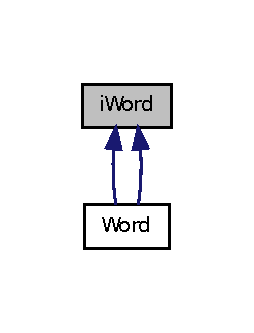
\includegraphics[width=122pt]{classiWord__inherit__graph}
\end{center}
\end{figure}
\subsection*{Public Member Functions}
\begin{DoxyCompactItemize}
\item 
virtual int \hyperlink{classiWord_a3349d0a243d3432bb35b76af8420b1d9}{toInt} () const =0
\begin{DoxyCompactList}\small\item\em \char`\"{}To non-\/negative Integer\char`\"{} \item\end{DoxyCompactList}\item 
virtual int \hyperlink{classiWord_a1377d01257b792c748b013be60b089e6}{toInt2Complement} () const =0
\begin{DoxyCompactList}\small\item\em \char`\"{}To Integer as 2's Complement\char`\"{} \item\end{DoxyCompactList}\item 
virtual std::string \hyperlink{classiWord_a0114861c4b660286834ad637f11dc4f4}{toStr} () const =0
\begin{DoxyCompactList}\small\item\em \char`\"{}To String\char`\"{} \item\end{DoxyCompactList}\item 
virtual std::string \hyperlink{classiWord_a7fc28d0251f8acb4dc3f388fc25c57d1}{toHex} () const =0
\begin{DoxyCompactList}\small\item\em \char`\"{}To Hexadecimal\char`\"{} \item\end{DoxyCompactList}\item 
virtual bool \hyperlink{classiWord_a6421bf139c6eb4044446997606cb65e7}{fromInt} (int)=0
\begin{DoxyCompactList}\small\item\em \char`\"{}From Integer\char`\"{} \item\end{DoxyCompactList}\item 
virtual bool \hyperlink{classiWord_ad8df9e06ccb87d1e65766120713ef545}{fromStr} (const std::string \&)=0
\begin{DoxyCompactList}\small\item\em \char`\"{}From String\char`\"{} \item\end{DoxyCompactList}\item 
virtual bool \hyperlink{classiWord_a0c08832b3e9b41073fc6666407ef8c53}{fromHex} (const std::string \&)=0
\begin{DoxyCompactList}\small\item\em \char`\"{}From Hexadecimal\char`\"{} \item\end{DoxyCompactList}\item 
virtual \hyperlink{classWord}{Word} \hyperlink{classiWord_a999c52ac2e7abf756eeb16fe5b31aad7}{Add} (const \hyperlink{classiWord}{iWord} \&) const =0
\begin{DoxyCompactList}\small\item\em Adds two words. \item\end{DoxyCompactList}\item 
virtual \hyperlink{classWord}{Word} \hyperlink{classiWord_a8dfb66b7cd91fe0a4169f071c1f9bc53}{operator+} (const \hyperlink{classiWord}{iWord} \&) const =0
\begin{DoxyCompactList}\small\item\em A standard addition operator. \item\end{DoxyCompactList}\item 
virtual \hyperlink{classWord}{Word} \hyperlink{classiWord_af69a5e10e094e3fc30fae0b651d95ea6}{Subtract} (const \hyperlink{classiWord}{iWord} \&) const =0
\begin{DoxyCompactList}\small\item\em Subtracts two words. \item\end{DoxyCompactList}\item 
virtual \hyperlink{classWord}{Word} \hyperlink{classiWord_a432fb05081debadb601d86cca05152c8}{operator-\/} (const \hyperlink{classiWord}{iWord} \&) const =0
\begin{DoxyCompactList}\small\item\em A standard subtraction operator. \item\end{DoxyCompactList}\item 
virtual \hyperlink{classWord}{Word} \hyperlink{classiWord_ae9f6bbc855712a208835d12cb3e40577}{And} (const \hyperlink{classiWord}{iWord} \&) const =0
\begin{DoxyCompactList}\small\item\em \char`\"{}And\char`\"{}s the bits of two words. \item\end{DoxyCompactList}\item 
\hypertarget{classiWord_a24a8821a44701deda1dd70972447172f}{
virtual \hyperlink{classWord}{Word} {\bfseries Or} (const \hyperlink{classiWord}{iWord} \&) const =0}
\label{classiWord_a24a8821a44701deda1dd70972447172f}

\item 
\hypertarget{classiWord_a6a7602a8220d84b5201a789b597fbbde}{
virtual \hyperlink{classWord}{Word} {\bfseries Not} () const =0}
\label{classiWord_a6a7602a8220d84b5201a789b597fbbde}

\item 
virtual void \hyperlink{classiWord_ab9f5df8ced4937c18f16784a98ecf95f}{copy} (const \hyperlink{classiWord}{iWord} \&)=0
\begin{DoxyCompactList}\small\item\em Copies a word. \item\end{DoxyCompactList}\item 
virtual \hyperlink{classWord}{Word} \& \hyperlink{classiWord_a45c9c82054bd2150b77d5f157734cb72}{operator=} (const \hyperlink{classWord}{Word})=0
\begin{DoxyCompactList}\small\item\em A standard assignment operator. \item\end{DoxyCompactList}\item 
virtual \hyperlink{classiWord}{iWord} \& \hyperlink{classiWord_af20040c25b79d2aeae41f1714fbb2cbc}{operator++} ()=0
\item 
virtual \hyperlink{classiWord}{iWord} \& \hyperlink{classiWord_a6777f6f41915179c4255d3647a9eb4b5}{operator++} (int)=0
\begin{DoxyCompactList}\small\item\em A standard post-\/increment operator. \item\end{DoxyCompactList}\item 
virtual bool \hyperlink{classiWord_a2bd140904379329b74c3e1af83eb3a85}{operator\mbox{[}$\,$\mbox{]}} (int) const =0
\begin{DoxyCompactList}\small\item\em An accessor to the \char`\"{}i\char`\"{}th bit of the value. \item\end{DoxyCompactList}\end{DoxyCompactItemize}


\subsection{Detailed Description}
The \hyperlink{classiWord}{iWord} interface class defines the a \char`\"{}word\char`\"{} of data on the Wi-\/11 Machine. The methods present in this inteface are meant to mimic the functionality of the Wi-\/11 machine, allowing for simplified execution of the instructions therein. As the size of a \char`\"{}word\char`\"{} depends on the architecture, classes implementing this interface should define the word length to be 16 bits in length. 

\subsection{Member Function Documentation}
\hypertarget{classiWord_a3349d0a243d3432bb35b76af8420b1d9}{
\index{iWord@{iWord}!toInt@{toInt}}
\index{toInt@{toInt}!iWord@{iWord}}
\subsubsection[{toInt}]{\setlength{\rightskip}{0pt plus 5cm}virtual int iWord::toInt (
\begin{DoxyParamCaption}
{}
\end{DoxyParamCaption}
) const\hspace{0.3cm}{\ttfamily  \mbox{[}pure virtual\mbox{]}}}}
\label{classiWord_a3349d0a243d3432bb35b76af8420b1d9}


\char`\"{}To non-\/negative Integer\char`\"{} 

\begin{DoxyPostcond}{Postcondition}
The value of the word is not changed. 
\end{DoxyPostcond}
\begin{DoxyReturn}{Returns}
The bits of the word interpreted as a positive integer value. 
\end{DoxyReturn}


Implemented in \hyperlink{classWord_a19303d963626549830a8da33d863bd6d}{Word}.

\hypertarget{classiWord_a1377d01257b792c748b013be60b089e6}{
\index{iWord@{iWord}!toInt2Complement@{toInt2Complement}}
\index{toInt2Complement@{toInt2Complement}!iWord@{iWord}}
\subsubsection[{toInt2Complement}]{\setlength{\rightskip}{0pt plus 5cm}virtual int iWord::toInt2Complement (
\begin{DoxyParamCaption}
{}
\end{DoxyParamCaption}
) const\hspace{0.3cm}{\ttfamily  \mbox{[}pure virtual\mbox{]}}}}
\label{classiWord_a1377d01257b792c748b013be60b089e6}


\char`\"{}To Integer as 2's Complement\char`\"{} 

\begin{DoxyPostcond}{Postcondition}
The value of the word is not changed. 
\end{DoxyPostcond}
\begin{DoxyReturn}{Returns}
The bits of the word interpreted as a signed (2's complement) integer value. 
\end{DoxyReturn}


Implemented in \hyperlink{classWord_a3d771d68afd4a70d279af8bd9cd6bef9}{Word}.

\hypertarget{classiWord_a0114861c4b660286834ad637f11dc4f4}{
\index{iWord@{iWord}!toStr@{toStr}}
\index{toStr@{toStr}!iWord@{iWord}}
\subsubsection[{toStr}]{\setlength{\rightskip}{0pt plus 5cm}virtual std::string iWord::toStr (
\begin{DoxyParamCaption}
{}
\end{DoxyParamCaption}
) const\hspace{0.3cm}{\ttfamily  \mbox{[}pure virtual\mbox{]}}}}
\label{classiWord_a0114861c4b660286834ad637f11dc4f4}


\char`\"{}To String\char`\"{} 

\begin{DoxyPostcond}{Postcondition}
The value of the word is not changed. 
\end{DoxyPostcond}
\begin{DoxyReturn}{Returns}
16 characters: each either a 1 or 0
\end{DoxyReturn}
\begin{DoxyParagraph}{Examples:}
If the object holds a (2's comp.) value 4: \char`\"{}0000000000000100\char`\"{}\par
 If the object holds a (2's comp.) value -\/1: \char`\"{}1111111111111111\char`\"{} 
\end{DoxyParagraph}


Implemented in \hyperlink{classWord_ac2ca49ef4da2fb57172fe057849e53fa}{Word}.

\hypertarget{classiWord_a7fc28d0251f8acb4dc3f388fc25c57d1}{
\index{iWord@{iWord}!toHex@{toHex}}
\index{toHex@{toHex}!iWord@{iWord}}
\subsubsection[{toHex}]{\setlength{\rightskip}{0pt plus 5cm}virtual std::string iWord::toHex (
\begin{DoxyParamCaption}
{}
\end{DoxyParamCaption}
) const\hspace{0.3cm}{\ttfamily  \mbox{[}pure virtual\mbox{]}}}}
\label{classiWord_a7fc28d0251f8acb4dc3f388fc25c57d1}


\char`\"{}To Hexadecimal\char`\"{} 

\begin{DoxyPostcond}{Postcondition}
The value of the word is not changed. 
\end{DoxyPostcond}
\begin{DoxyReturn}{Returns}
\char`\"{}0x\char`\"{} + $<$4 characters in the range \mbox{[}0-\/9\mbox{]},\mbox{[}A-\/F\mbox{]}$>$
\end{DoxyReturn}
\begin{DoxyParagraph}{Examples:}
If the object holds (2's comp.) value 8: \char`\"{}0x0008\char`\"{}\par
 If the object holds (2's comp.) value -\/2: \char`\"{}0xFFFE\char`\"{} 
\end{DoxyParagraph}


Implemented in \hyperlink{classWord_ab797467868642bb096bc4c9b1ed0a2f0}{Word}.

\hypertarget{classiWord_a6421bf139c6eb4044446997606cb65e7}{
\index{iWord@{iWord}!fromInt@{fromInt}}
\index{fromInt@{fromInt}!iWord@{iWord}}
\subsubsection[{fromInt}]{\setlength{\rightskip}{0pt plus 5cm}virtual bool iWord::fromInt (
\begin{DoxyParamCaption}
\item[{int}]{}
\end{DoxyParamCaption}
)\hspace{0.3cm}{\ttfamily  \mbox{[}pure virtual\mbox{]}}}}
\label{classiWord_a6421bf139c6eb4044446997606cb65e7}


\char`\"{}From Integer\char`\"{} 


\begin{DoxyParams}[1]{Parameters}
\mbox{\tt in}  & {\em value} & The value to be stored into the word. \\
\hline
\end{DoxyParams}
\begin{DoxyPostcond}{Postcondition}
\char`\"{}value\char`\"{} is not changed. 
\end{DoxyPostcond}
\begin{DoxyReturn}{Returns}
True if and only if \char`\"{}value\char`\"{} can be represented in 16 bits
\end{DoxyReturn}
When this function returns \char`\"{}False\char`\"{}, the value of the word is unchanged.\par
 Otherwise, the word now holds the value \char`\"{}value\char`\"{}. 

Implemented in \hyperlink{classWord_ad6499f93b487d6d550a3fd4adcee9c8d}{Word}.

\hypertarget{classiWord_ad8df9e06ccb87d1e65766120713ef545}{
\index{iWord@{iWord}!fromStr@{fromStr}}
\index{fromStr@{fromStr}!iWord@{iWord}}
\subsubsection[{fromStr}]{\setlength{\rightskip}{0pt plus 5cm}virtual bool iWord::fromStr (
\begin{DoxyParamCaption}
\item[{const std::string \&}]{}
\end{DoxyParamCaption}
)\hspace{0.3cm}{\ttfamily  \mbox{[}pure virtual\mbox{]}}}}
\label{classiWord_ad8df9e06ccb87d1e65766120713ef545}


\char`\"{}From String\char`\"{} 


\begin{DoxyParams}[1]{Parameters}
\mbox{\tt in}  & {\em str} & A string of characters meant to represent a \char`\"{}word\char`\"{} to be stored. \\
\hline
\end{DoxyParams}
\begin{DoxyPostcond}{Postcondition}
\char`\"{}str\char`\"{} is not changed. 
\end{DoxyPostcond}
\begin{DoxyReturn}{Returns}
True if and only if \char`\"{}str\char`\"{} is well-\/formed (as defined in \hyperlink{classiWord_a0114861c4b660286834ad637f11dc4f4}{toStr()}).
\end{DoxyReturn}
When this function returns \char`\"{}False\char`\"{}, the value of the word is unchanged.\par
 Otherwise, the word now holds the value \char`\"{}str\char`\"{}. 

Implemented in \hyperlink{classWord_a614b52f3312d82ac5681403651040714}{Word}.

\hypertarget{classiWord_a0c08832b3e9b41073fc6666407ef8c53}{
\index{iWord@{iWord}!fromHex@{fromHex}}
\index{fromHex@{fromHex}!iWord@{iWord}}
\subsubsection[{fromHex}]{\setlength{\rightskip}{0pt plus 5cm}virtual bool iWord::fromHex (
\begin{DoxyParamCaption}
\item[{const std::string \&}]{}
\end{DoxyParamCaption}
)\hspace{0.3cm}{\ttfamily  \mbox{[}pure virtual\mbox{]}}}}
\label{classiWord_a0c08832b3e9b41073fc6666407ef8c53}


\char`\"{}From Hexadecimal\char`\"{} 


\begin{DoxyParams}[1]{Parameters}
\mbox{\tt in}  & {\em str} & A string of characters meant to represent a \char`\"{}word\char`\"{} to be stored. \\
\hline
\end{DoxyParams}
\begin{DoxyPostcond}{Postcondition}
\char`\"{}str\char`\"{} is not changed. 
\end{DoxyPostcond}
\begin{DoxyReturn}{Returns}
True if and only if \char`\"{}str\char`\"{} is well-\/formed (as defined in \hyperlink{classiWord_a7fc28d0251f8acb4dc3f388fc25c57d1}{toHex()}).
\end{DoxyReturn}
When this function returns \char`\"{}False\char`\"{}, the value of the word is unchanged.\par
 Otherwise, the word now holds the value \char`\"{}str\char`\"{}. 

Implemented in \hyperlink{classWord_a4e26eb82e8f7426dd46be2bbec9e41c5}{Word}.

\hypertarget{classiWord_a999c52ac2e7abf756eeb16fe5b31aad7}{
\index{iWord@{iWord}!Add@{Add}}
\index{Add@{Add}!iWord@{iWord}}
\subsubsection[{Add}]{\setlength{\rightskip}{0pt plus 5cm}virtual {\bf Word} iWord::Add (
\begin{DoxyParamCaption}
\item[{const {\bf iWord} \&}]{}
\end{DoxyParamCaption}
) const\hspace{0.3cm}{\ttfamily  \mbox{[}pure virtual\mbox{]}}}}
\label{classiWord_a999c52ac2e7abf756eeb16fe5b31aad7}


Adds two words. 


\begin{DoxyParams}[1]{Parameters}
\mbox{\tt in}  & {\em w} & A word value to be added. \\
\hline
\end{DoxyParams}
\begin{DoxyPostcond}{Postcondition}
Both \char`\"{}w\char`\"{} and the calling object do not change. 
\end{DoxyPostcond}
\begin{DoxyReturn}{Returns}
A new \char`\"{}Word\char`\"{} object containing result of adding \char`\"{}w\char`\"{} and the calling object.
\end{DoxyReturn}
\begin{DoxyNote}{Note}
The addition is carried out with no regard to logical overflow. 
\end{DoxyNote}


Implemented in \hyperlink{classWord_a5cb9115a6cee6666e88390e56eb32071}{Word}.

\hypertarget{classiWord_a8dfb66b7cd91fe0a4169f071c1f9bc53}{
\index{iWord@{iWord}!operator+@{operator+}}
\index{operator+@{operator+}!iWord@{iWord}}
\subsubsection[{operator+}]{\setlength{\rightskip}{0pt plus 5cm}virtual {\bf Word} iWord::operator+ (
\begin{DoxyParamCaption}
\item[{const {\bf iWord} \&}]{}
\end{DoxyParamCaption}
) const\hspace{0.3cm}{\ttfamily  \mbox{[}pure virtual\mbox{]}}}}
\label{classiWord_a8dfb66b7cd91fe0a4169f071c1f9bc53}


A standard addition operator. 

\begin{DoxyNote}{Note}
\char`\"{}result = p + w\char`\"{} is equivalent to \char`\"{}result = p.Add(w)\char`\"{}. 
\end{DoxyNote}


Implemented in \hyperlink{classWord_a88e945efd81d13e15adb1ed9e4e95a5a}{Word}.

\hypertarget{classiWord_af69a5e10e094e3fc30fae0b651d95ea6}{
\index{iWord@{iWord}!Subtract@{Subtract}}
\index{Subtract@{Subtract}!iWord@{iWord}}
\subsubsection[{Subtract}]{\setlength{\rightskip}{0pt plus 5cm}virtual {\bf Word} iWord::Subtract (
\begin{DoxyParamCaption}
\item[{const {\bf iWord} \&}]{}
\end{DoxyParamCaption}
) const\hspace{0.3cm}{\ttfamily  \mbox{[}pure virtual\mbox{]}}}}
\label{classiWord_af69a5e10e094e3fc30fae0b651d95ea6}


Subtracts two words. 


\begin{DoxyParams}[1]{Parameters}
\mbox{\tt in}  & {\em w} & A word value to be subtracted. \\
\hline
\end{DoxyParams}
\begin{DoxyPostcond}{Postcondition}
Both \char`\"{}w\char`\"{} and the calling object do not change. 
\end{DoxyPostcond}
\begin{DoxyReturn}{Returns}
A new \char`\"{}Word\char`\"{} object containing the result of subtracting \char`\"{}w\char`\"{} from the calling object.
\end{DoxyReturn}
\begin{DoxyNote}{Note}
The subtraction is carried out with no regard for logical overflow. 
\end{DoxyNote}


Implemented in \hyperlink{classWord_a3ef457fb6f6ce54f5e98a83db4ae4472}{Word}.

\hypertarget{classiWord_a432fb05081debadb601d86cca05152c8}{
\index{iWord@{iWord}!operator-\/@{operator-\/}}
\index{operator-\/@{operator-\/}!iWord@{iWord}}
\subsubsection[{operator-\/}]{\setlength{\rightskip}{0pt plus 5cm}virtual {\bf Word} iWord::operator-\/ (
\begin{DoxyParamCaption}
\item[{const {\bf iWord} \&}]{}
\end{DoxyParamCaption}
) const\hspace{0.3cm}{\ttfamily  \mbox{[}pure virtual\mbox{]}}}}
\label{classiWord_a432fb05081debadb601d86cca05152c8}


A standard subtraction operator. 

\begin{DoxyNote}{Note}
\char`\"{}result = p -\/ w\char`\"{} is equivalent to \char`\"{}result = p.Subtract(w)\char`\"{}. 
\end{DoxyNote}


Implemented in \hyperlink{classWord_a9ec270f103a3a755bd7b627e4b899bb4}{Word}.

\hypertarget{classiWord_ae9f6bbc855712a208835d12cb3e40577}{
\index{iWord@{iWord}!And@{And}}
\index{And@{And}!iWord@{iWord}}
\subsubsection[{And}]{\setlength{\rightskip}{0pt plus 5cm}virtual {\bf Word} iWord::And (
\begin{DoxyParamCaption}
\item[{const {\bf iWord} \&}]{}
\end{DoxyParamCaption}
) const\hspace{0.3cm}{\ttfamily  \mbox{[}pure virtual\mbox{]}}}}
\label{classiWord_ae9f6bbc855712a208835d12cb3e40577}


\char`\"{}And\char`\"{}s the bits of two words. 


\begin{DoxyParams}[1]{Parameters}
\mbox{\tt in}  & {\em w} & A word value to be \char`\"{}and\char`\"{}ed. \\
\hline
\end{DoxyParams}
\begin{DoxyPostcond}{Postcondition}
Both \char`\"{}w\char`\"{} and the calling object do not change. 
\end{DoxyPostcond}
\begin{DoxyReturn}{Returns}
A new \char`\"{}Word\char`\"{} object containing the result of performing a bit-\/wise and on \char`\"{}w\char`\"{} and the calling object. 
\end{DoxyReturn}


Implemented in \hyperlink{classWord_a4e1926ab5f4af7b63ec1bf4fadf873ad}{Word}.

\hypertarget{classiWord_ab9f5df8ced4937c18f16784a98ecf95f}{
\index{iWord@{iWord}!copy@{copy}}
\index{copy@{copy}!iWord@{iWord}}
\subsubsection[{copy}]{\setlength{\rightskip}{0pt plus 5cm}virtual void iWord::copy (
\begin{DoxyParamCaption}
\item[{const {\bf iWord} \&}]{}
\end{DoxyParamCaption}
)\hspace{0.3cm}{\ttfamily  \mbox{[}pure virtual\mbox{]}}}}
\label{classiWord_ab9f5df8ced4937c18f16784a98ecf95f}


Copies a word. 


\begin{DoxyParams}[1]{Parameters}
\mbox{\tt out}  & {\em The} & value to be copied. \\
\hline
\end{DoxyParams}
\begin{DoxyPostcond}{Postcondition}
The caller equals that parameter.
\end{DoxyPostcond}
Equivalent to the assignment \char`\"{}caller = parameter\char`\"{}. 

Implemented in \hyperlink{classWord_abb97142e332c7cc25d2a0c2bdb6c3d9b}{Word}.

\hypertarget{classiWord_a45c9c82054bd2150b77d5f157734cb72}{
\index{iWord@{iWord}!operator=@{operator=}}
\index{operator=@{operator=}!iWord@{iWord}}
\subsubsection[{operator=}]{\setlength{\rightskip}{0pt plus 5cm}virtual {\bf Word}\& iWord::operator= (
\begin{DoxyParamCaption}
\item[{const }]{ Word}
\end{DoxyParamCaption}
)\hspace{0.3cm}{\ttfamily  \mbox{[}pure virtual\mbox{]}}}}
\label{classiWord_a45c9c82054bd2150b77d5f157734cb72}


A standard assignment operator. 


\begin{DoxyParams}[1]{Parameters}
\mbox{\tt in}  & {\em The} & value to be copied. \\
\hline
\end{DoxyParams}
\begin{DoxyReturn}{Returns}
A copy of the parameter.
\end{DoxyReturn}
The return value and parameter here must be declared as \char`\"{}Word\char`\"{}s as C++ does not work well with polymorphic assignment operators. 

Implemented in \hyperlink{classWord_a2ae41869cb0f1855fc18c6bce05f7c4d}{Word}.

\hypertarget{classiWord_af20040c25b79d2aeae41f1714fbb2cbc}{
\index{iWord@{iWord}!operator++@{operator++}}
\index{operator++@{operator++}!iWord@{iWord}}
\subsubsection[{operator++}]{\setlength{\rightskip}{0pt plus 5cm}virtual {\bf iWord}\& iWord::operator++ (
\begin{DoxyParamCaption}
{}
\end{DoxyParamCaption}
)\hspace{0.3cm}{\ttfamily  \mbox{[}pure virtual\mbox{]}}}}
\label{classiWord_af20040c25b79d2aeae41f1714fbb2cbc}
A standard pre-\/increment operator. \begin{DoxyReturn}{Returns}
A reference to itself.
\end{DoxyReturn}
The object increments its value BEFORE the execution of the current line. 

Implemented in \hyperlink{classWord_a3837f49bcb44597e6d738ccb0eeed144}{Word}.

\hypertarget{classiWord_a6777f6f41915179c4255d3647a9eb4b5}{
\index{iWord@{iWord}!operator++@{operator++}}
\index{operator++@{operator++}!iWord@{iWord}}
\subsubsection[{operator++}]{\setlength{\rightskip}{0pt plus 5cm}virtual {\bf iWord}\& iWord::operator++ (
\begin{DoxyParamCaption}
\item[{int}]{}
\end{DoxyParamCaption}
)\hspace{0.3cm}{\ttfamily  \mbox{[}pure virtual\mbox{]}}}}
\label{classiWord_a6777f6f41915179c4255d3647a9eb4b5}


A standard post-\/increment operator. 

\begin{DoxyReturn}{Returns}
A reference to itself.
\end{DoxyReturn}
The object increments its value AFTER the execution of the current line. 

Implemented in \hyperlink{classWord_ae921b75d263be790fd150c5962445163}{Word}.

\hypertarget{classiWord_a2bd140904379329b74c3e1af83eb3a85}{
\index{iWord@{iWord}!operator\mbox{[}\mbox{]}@{operator[]}}
\index{operator\mbox{[}\mbox{]}@{operator[]}!iWord@{iWord}}
\subsubsection[{operator[]}]{\setlength{\rightskip}{0pt plus 5cm}virtual bool iWord::operator\mbox{[}$\,$\mbox{]} (
\begin{DoxyParamCaption}
\item[{int}]{}
\end{DoxyParamCaption}
) const\hspace{0.3cm}{\ttfamily  \mbox{[}pure virtual\mbox{]}}}}
\label{classiWord_a2bd140904379329b74c3e1af83eb3a85}


An accessor to the \char`\"{}i\char`\"{}th bit of the value. 


\begin{DoxyParams}[1]{Parameters}
\mbox{\tt in}  & {\em The} & index of the bit in question. \\
\hline
\end{DoxyParams}
\begin{DoxyPrecond}{Precondition}
The index must be less than the size of a word, ie. 16. 
\end{DoxyPrecond}
\begin{DoxyReturn}{Returns}
True $<$=$>$ 1, False $<$=$>$ 0.
\end{DoxyReturn}
The number of the bits starts at zero and rises into the more significant bits. \begin{DoxyParagraph}{Examples:}
If the object holds a value of 4 (0...100 in binary): num\mbox{[}2\mbox{]} = 1.\par
 If it holds a value of 1 (0...001 in binary): num\mbox{[}0\mbox{]} = 1.\par
 If it holds a negative value (Starting with a 1 in 2's complement): num\mbox{[}15\mbox{]} = 1. 
\end{DoxyParagraph}


Implemented in \hyperlink{classWord_ab0f10ac1a0397559b859774b503538fe}{Word}.



The documentation for this class was generated from the following file:\begin{DoxyCompactItemize}
\item 
\hyperlink{iWord_8h}{iWord.h}\end{DoxyCompactItemize}

\hypertarget{classLoader}{
\section{Loader Class Reference}
\label{classLoader}\index{Loader@{Loader}}
}


Implements \hyperlink{classiLoader}{iLoader}.  




Collaboration diagram for Loader:\nopagebreak
\begin{figure}[H]
\begin{center}
\leavevmode
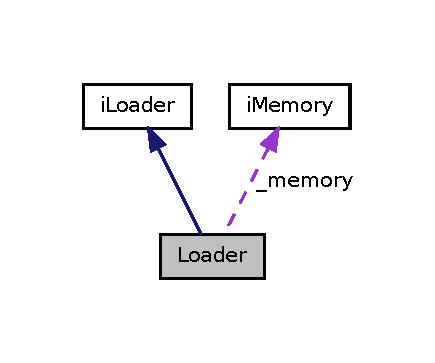
\includegraphics[width=209pt]{classLoader__coll__graph}
\end{center}
\end{figure}
\subsection*{Public Member Functions}
\begin{DoxyCompactItemize}
\item 
\hypertarget{classLoader_acc964f5d36a91baa584a8ecfa1e3945f}{
Codes::RESULT {\bfseries Load} (const char $\ast$filename, \hyperlink{classiWord}{iWord} \&PC\_\-address) const }
\label{classLoader_acc964f5d36a91baa584a8ecfa1e3945f}

\item 
\hyperlink{classLoader_ab2155ac99a41ba255c88161b9a3d218a}{Loader} (\hyperlink{classiMemory}{iMemory} $\ast$mem)
\begin{DoxyCompactList}\small\item\em Set which \hyperlink{classMemory}{Memory} object is to be initialized by this object. \item\end{DoxyCompactList}\end{DoxyCompactItemize}
\subsection*{Private Attributes}
\begin{DoxyCompactItemize}
\item 
\hypertarget{classLoader_a5e7c0fcca7b8bf89db54e1b65d28e309}{
\hyperlink{classiMemory}{iMemory} $\ast$ \hyperlink{classLoader_a5e7c0fcca7b8bf89db54e1b65d28e309}{\_\-memory}}
\label{classLoader_a5e7c0fcca7b8bf89db54e1b65d28e309}

\begin{DoxyCompactList}\small\item\em The reference to \hyperlink{classMemory}{Memory}. \item\end{DoxyCompactList}\end{DoxyCompactItemize}


\subsection{Detailed Description}
Implements \hyperlink{classiLoader}{iLoader}. 

\subsection{Constructor \& Destructor Documentation}
\hypertarget{classLoader_ab2155ac99a41ba255c88161b9a3d218a}{
\index{Loader@{Loader}!Loader@{Loader}}
\index{Loader@{Loader}!Loader@{Loader}}
\subsubsection[{Loader}]{\setlength{\rightskip}{0pt plus 5cm}Loader::Loader (
\begin{DoxyParamCaption}
\item[{{\bf iMemory} $\ast$}]{ mem}
\end{DoxyParamCaption}
)}}
\label{classLoader_ab2155ac99a41ba255c88161b9a3d218a}


Set which \hyperlink{classMemory}{Memory} object is to be initialized by this object. 


\begin{DoxyParams}[1]{Parameters}
\mbox{\tt in}  & {\em mem} & The address where memory is located.\\
\hline
\end{DoxyParams}
\begin{DoxyNote}{Note}
Without this there would be nowhere to load the instructions. 
\end{DoxyNote}

\hypertarget{classMemory}{
\section{Memory Class Reference}
\label{classMemory}\index{Memory@{Memory}}
}


Inheritance diagram for Memory:
\nopagebreak
\begin{figure}[H]
\begin{center}
\leavevmode
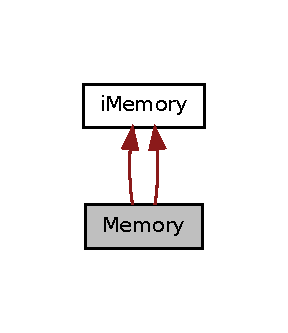
\includegraphics[width=138pt]{classMemory__inherit__graph}
\end{center}
\end{figure}


Collaboration diagram for Memory:
\nopagebreak
\begin{figure}[H]
\begin{center}
\leavevmode
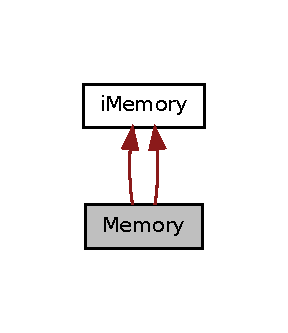
\includegraphics[width=138pt]{classMemory__coll__graph}
\end{center}
\end{figure}
\subsection*{Public Member Functions}
\begin{DoxyCompactItemize}
\item 
virtual Codes::RESULT \hyperlink{classMemory_a80cd994d4833dde66b8005184e510dda}{Reserve} (const \hyperlink{classiWord}{iWord} \&initial\_\-address, const \hyperlink{classiWord}{iWord} \&length)
\begin{DoxyCompactList}\small\item\em Reserves an initial section of memory for instructions. \item\end{DoxyCompactList}\item 
virtual \hyperlink{classWord}{Word} \hyperlink{classMemory_aca021609915080b38ca1b00d9b416e80}{Load} (const \hyperlink{classiWord}{iWord} \&) const 
\begin{DoxyCompactList}\small\item\em Performs a load. \item\end{DoxyCompactList}\item 
virtual Codes::RESULT \hyperlink{classMemory_a23703464fb24710d09be1b2010e79edc}{Store} (const \hyperlink{classiWord}{iWord} \&address, const \hyperlink{classWord}{Word} \&value)
\begin{DoxyCompactList}\small\item\em Peforms a store. \item\end{DoxyCompactList}\item 
virtual Codes::RESULT \hyperlink{classMemory_afe683401c1656b0a077d5f666f9c8d51}{Reserve} (const \hyperlink{classiWord}{iWord} \&initial\_\-address, const \hyperlink{classiWord}{iWord} \&length)
\begin{DoxyCompactList}\small\item\em Reserves an initial section of memory for instructions. \item\end{DoxyCompactList}\item 
virtual \hyperlink{classWord}{Word} \hyperlink{classMemory_af043b481b061644f9ff6cd7288655c93}{Load} (const \hyperlink{classiWord}{iWord} \&) const 
\begin{DoxyCompactList}\small\item\em Performs a load. \item\end{DoxyCompactList}\item 
virtual Codes::RESULT \hyperlink{classMemory_a100745221ade9b322743514d91fcce23}{Store} (const \hyperlink{classiWord}{iWord} \&address, const \hyperlink{classWord}{Word} \&value)
\begin{DoxyCompactList}\small\item\em Peforms a store. \item\end{DoxyCompactList}\end{DoxyCompactItemize}
\subsection*{Private Attributes}
\begin{DoxyCompactItemize}
\item 
\hypertarget{classMemory_a261c779e202d16009dd48c68291266f9}{
std::vector$<$ \hyperlink{classWord}{Word} $\ast$ $>$ \hyperlink{classMemory_a261c779e202d16009dd48c68291266f9}{\_\-bounded\_\-memory}}
\label{classMemory_a261c779e202d16009dd48c68291266f9}

\begin{DoxyCompactList}\small\item\em Provide constant time access to reserved memory. \item\end{DoxyCompactList}\item 
\hypertarget{classMemory_adceb29287c4850dc78b4a66cc0890d47}{
std::vector$<$ int $>$ \hyperlink{classMemory_adceb29287c4850dc78b4a66cc0890d47}{\_\-segment\_\-offsets}}
\label{classMemory_adceb29287c4850dc78b4a66cc0890d47}

\begin{DoxyCompactList}\small\item\em Keep track of the initial addresses. \item\end{DoxyCompactList}\item 
\hypertarget{classMemory_a8a5f79ee8ee270287a668383ec8f4a6d}{
std::vector$<$ int $>$ \hyperlink{classMemory_a8a5f79ee8ee270287a668383ec8f4a6d}{\_\-segment\_\-lengths}}
\label{classMemory_a8a5f79ee8ee270287a668383ec8f4a6d}

\begin{DoxyCompactList}\small\item\em Keep track of the size of reserved memory. \item\end{DoxyCompactList}\item 
\hypertarget{classMemory_a390295664efe18aa33298ead1004c442}{
std::map$<$ int, \hyperlink{classWord}{Word} $>$ \hyperlink{classMemory_a390295664efe18aa33298ead1004c442}{\_\-unbounded\_\-memory}}
\label{classMemory_a390295664efe18aa33298ead1004c442}

\begin{DoxyCompactList}\small\item\em Map out-\/of-\/bounds values to new Words. \item\end{DoxyCompactList}\end{DoxyCompactItemize}


\subsection{Member Function Documentation}
\hypertarget{classMemory_a80cd994d4833dde66b8005184e510dda}{
\index{Memory@{Memory}!Reserve@{Reserve}}
\index{Reserve@{Reserve}!Memory@{Memory}}
\subsubsection[{Reserve}]{\setlength{\rightskip}{0pt plus 5cm}RESULT Memory::Reserve (
\begin{DoxyParamCaption}
\item[{const {\bf iWord} \&}]{ initial\_\-address, }
\item[{const {\bf iWord} \&}]{ length}
\end{DoxyParamCaption}
)\hspace{0.3cm}{\ttfamily  \mbox{[}virtual\mbox{]}}}}
\label{classMemory_a80cd994d4833dde66b8005184e510dda}


Reserves an initial section of memory for instructions. 


\begin{DoxyParams}[1]{Parameters}
\mbox{\tt in}  & {\em initial\_\-address} & The smallest address for the instruction memory. \\
\hline
\mbox{\tt in}  & {\em length} & The number of addresses to reserve. \\
\hline
\end{DoxyParams}
\begin{DoxyReturn}{Returns}
SUCCESS or, if something goes wrong, an appropriate error code.
\end{DoxyReturn}
The memory reserved here is dynamically allocated and provides constant-\/time access to addresses \char`\"{}initial\_\-address\char`\"{} through \char`\"{}initial\_\-address\char`\"{}+\char`\"{}length\char`\"{}-\/1. 

Implements \hyperlink{classiMemory_a27750e74d09fb473c163a4cc4c3e697b}{iMemory}.

\hypertarget{classMemory_aca021609915080b38ca1b00d9b416e80}{
\index{Memory@{Memory}!Load@{Load}}
\index{Load@{Load}!Memory@{Memory}}
\subsubsection[{Load}]{\setlength{\rightskip}{0pt plus 5cm}{\bf Word} Memory::Load (
\begin{DoxyParamCaption}
\item[{const {\bf iWord} \&}]{ w}
\end{DoxyParamCaption}
) const\hspace{0.3cm}{\ttfamily  \mbox{[}virtual\mbox{]}}}}
\label{classMemory_aca021609915080b38ca1b00d9b416e80}


Performs a load. 


\begin{DoxyParams}[1]{Parameters}
\mbox{\tt in}  & {\em w} & The address from which to load data. \\
\hline
\end{DoxyParams}
\begin{DoxyReturn}{Returns}
The data stored a address \char`\"{}w\char`\"{}.
\end{DoxyReturn}
\begin{DoxyNote}{Note}
If \char`\"{}w\char`\"{} is in the range created by Reserve(), it can be accessed in constant time. Otherwise, a maximum of nlogn time is required if n is the size of memory initialized outside of these boundaries. 
\end{DoxyNote}


Implements \hyperlink{classiMemory_a3352ba391fc9b69a0b8691b2d585596a}{iMemory}.

\hypertarget{classMemory_a23703464fb24710d09be1b2010e79edc}{
\index{Memory@{Memory}!Store@{Store}}
\index{Store@{Store}!Memory@{Memory}}
\subsubsection[{Store}]{\setlength{\rightskip}{0pt plus 5cm}RESULT Memory::Store (
\begin{DoxyParamCaption}
\item[{const {\bf iWord} \&}]{ address, }
\item[{const {\bf Word} \&}]{ value}
\end{DoxyParamCaption}
)\hspace{0.3cm}{\ttfamily  \mbox{[}virtual\mbox{]}}}}
\label{classMemory_a23703464fb24710d09be1b2010e79edc}


Peforms a store. 


\begin{DoxyParams}[1]{Parameters}
\mbox{\tt in}  & {\em address} & The address to store the data. \\
\hline
\mbox{\tt in}  & {\em value} & The data to store at \char`\"{}address\char`\"{}. \\
\hline
\end{DoxyParams}
\begin{DoxyReturn}{Returns}
SUCCESS or, if something went wrong, an appropriate error code.
\end{DoxyReturn}
\begin{DoxyNote}{Note}
The efficiency constraints in Load() apply here as well. 
\end{DoxyNote}


Implements \hyperlink{classiMemory_a2632c9999797b0799a7d6b0a59bfa91a}{iMemory}.

\hypertarget{classMemory_afe683401c1656b0a077d5f666f9c8d51}{
\index{Memory@{Memory}!Reserve@{Reserve}}
\index{Reserve@{Reserve}!Memory@{Memory}}
\subsubsection[{Reserve}]{\setlength{\rightskip}{0pt plus 5cm}virtual Codes::RESULT Memory::Reserve (
\begin{DoxyParamCaption}
\item[{const {\bf iWord} \&}]{ initial\_\-address, }
\item[{const {\bf iWord} \&}]{ length}
\end{DoxyParamCaption}
)\hspace{0.3cm}{\ttfamily  \mbox{[}virtual\mbox{]}}}}
\label{classMemory_afe683401c1656b0a077d5f666f9c8d51}


Reserves an initial section of memory for instructions. 


\begin{DoxyParams}[1]{Parameters}
\mbox{\tt in}  & {\em initial\_\-address} & The smallest address for the instruction memory. \\
\hline
\mbox{\tt in}  & {\em length} & The number of addresses to reserve. \\
\hline
\end{DoxyParams}
\begin{DoxyReturn}{Returns}
SUCCESS or, if something goes wrong, an appropriate error code.
\end{DoxyReturn}
The memory reserved here is dynamically allocated and provides constant-\/time access to addresses \char`\"{}initial\_\-address\char`\"{} through \char`\"{}initial\_\-address\char`\"{}+\char`\"{}length\char`\"{}-\/1. 

Implements \hyperlink{classiMemory_a27750e74d09fb473c163a4cc4c3e697b}{iMemory}.

\hypertarget{classMemory_af043b481b061644f9ff6cd7288655c93}{
\index{Memory@{Memory}!Load@{Load}}
\index{Load@{Load}!Memory@{Memory}}
\subsubsection[{Load}]{\setlength{\rightskip}{0pt plus 5cm}virtual {\bf Word} Memory::Load (
\begin{DoxyParamCaption}
\item[{const {\bf iWord} \&}]{ w}
\end{DoxyParamCaption}
) const\hspace{0.3cm}{\ttfamily  \mbox{[}virtual\mbox{]}}}}
\label{classMemory_af043b481b061644f9ff6cd7288655c93}


Performs a load. 


\begin{DoxyParams}[1]{Parameters}
\mbox{\tt in}  & {\em w} & The address from which to load data. \\
\hline
\end{DoxyParams}
\begin{DoxyReturn}{Returns}
The data stored a address \char`\"{}w\char`\"{}.
\end{DoxyReturn}
\begin{DoxyNote}{Note}
If \char`\"{}w\char`\"{} is in the range created by Reserve(), it can be accessed in constant time. Otherwise, a maximum of nlogn time is required if n is the size of memory initialized outside of these boundaries. 
\end{DoxyNote}


Implements \hyperlink{classiMemory_a3352ba391fc9b69a0b8691b2d585596a}{iMemory}.

\hypertarget{classMemory_a100745221ade9b322743514d91fcce23}{
\index{Memory@{Memory}!Store@{Store}}
\index{Store@{Store}!Memory@{Memory}}
\subsubsection[{Store}]{\setlength{\rightskip}{0pt plus 5cm}virtual Codes::RESULT Memory::Store (
\begin{DoxyParamCaption}
\item[{const {\bf iWord} \&}]{ address, }
\item[{const {\bf Word} \&}]{ value}
\end{DoxyParamCaption}
)\hspace{0.3cm}{\ttfamily  \mbox{[}virtual\mbox{]}}}}
\label{classMemory_a100745221ade9b322743514d91fcce23}


Peforms a store. 


\begin{DoxyParams}[1]{Parameters}
\mbox{\tt in}  & {\em address} & The address to store the data. \\
\hline
\mbox{\tt in}  & {\em value} & The data to store at \char`\"{}address\char`\"{}. \\
\hline
\end{DoxyParams}
\begin{DoxyReturn}{Returns}
SUCCESS or, if something went wrong, an appropriate error code.
\end{DoxyReturn}
\begin{DoxyNote}{Note}
The efficiency constraints in Load() apply here as well. 
\end{DoxyNote}


Implements \hyperlink{classiMemory_a2632c9999797b0799a7d6b0a59bfa91a}{iMemory}.


\hypertarget{structObjectData}{
\section{ObjectData Struct Reference}
\label{structObjectData}\index{ObjectData@{ObjectData}}
}
\subsection*{Public Attributes}
\begin{DoxyCompactItemize}
\item 
\hypertarget{structObjectData_a77f1a74deb864606b1b5cc115c2a99a5}{
char {\bfseries type}}
\label{structObjectData_a77f1a74deb864606b1b5cc115c2a99a5}

\item 
\hypertarget{structObjectData_af755ea276bafd67e377e869950c1eb48}{
std::vector$<$ std::string $>$ {\bfseries data}}
\label{structObjectData_af755ea276bafd67e377e869950c1eb48}

\end{DoxyCompactItemize}

\hypertarget{classObjParser}{
\section{ObjParser Class Reference}
\label{classObjParser}\index{ObjParser@{ObjParser}}
}


Implements \hyperlink{classiObjParser}{iObjParser}.  




Collaboration diagram for ObjParser:\nopagebreak
\begin{figure}[H]
\begin{center}
\leavevmode
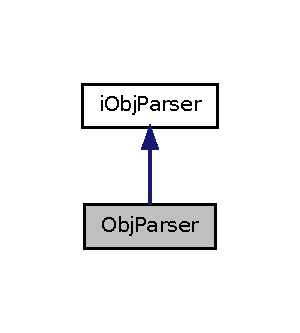
\includegraphics[width=144pt]{classObjParser__coll__graph}
\end{center}
\end{figure}
\subsection*{Public Member Functions}
\begin{DoxyCompactItemize}
\item 
\hyperlink{structObjectData}{ObjectData} \hyperlink{classObjParser_a653f83071fd63e3fdf04f28699f2fff5}{GetNext} ()
\begin{DoxyCompactList}\small\item\em Reads the next line from the current object file and parses it into an \hyperlink{structObjectData}{ObjectData} struct for use by the loader. \item\end{DoxyCompactList}\item 
Codes::RESULT \hyperlink{classObjParser_ae8d9939f390a68901e256d8a3187c24a}{Initialize} (const char $\ast$name)
\begin{DoxyCompactList}\small\item\em Closes \_\-fileStream if necessary, then opens the file defined by \char`\"{}name\char`\"{}. \item\end{DoxyCompactList}\item 
\hypertarget{classObjParser_aea8cf97813333011fcfa8ed67327009d}{
\hyperlink{classObjParser_aea8cf97813333011fcfa8ed67327009d}{$\sim$ObjParser} ()}
\label{classObjParser_aea8cf97813333011fcfa8ed67327009d}

\begin{DoxyCompactList}\small\item\em Closes a file, if necessary, when an \hyperlink{classiObjParser}{iObjParser} object goes out of scope. \item\end{DoxyCompactList}\end{DoxyCompactItemize}
\subsection*{Private Attributes}
\begin{DoxyCompactItemize}
\item 
\hypertarget{classObjParser_a50f5e135e982471969c63796becf20d6}{
std::ifstream \hyperlink{classObjParser_a50f5e135e982471969c63796becf20d6}{\_\-fileStream}}
\label{classObjParser_a50f5e135e982471969c63796becf20d6}

\begin{DoxyCompactList}\small\item\em Maintains an input stream from the object file specified by the \char`\"{}name\char`\"{} parameter to Initialize. \item\end{DoxyCompactList}\end{DoxyCompactItemize}


\subsection{Detailed Description}
Implements \hyperlink{classiObjParser}{iObjParser}. 

\subsection{Member Function Documentation}
\hypertarget{classObjParser_ae8d9939f390a68901e256d8a3187c24a}{
\index{ObjParser@{ObjParser}!Initialize@{Initialize}}
\index{Initialize@{Initialize}!ObjParser@{ObjParser}}
\subsubsection[{Initialize}]{\setlength{\rightskip}{0pt plus 5cm}Codes::RESULT ObjParser::Initialize (
\begin{DoxyParamCaption}
\item[{const char $\ast$}]{ name}
\end{DoxyParamCaption}
)\hspace{0.3cm}{\ttfamily  \mbox{[}virtual\mbox{]}}}}
\label{classObjParser_ae8d9939f390a68901e256d8a3187c24a}


Closes \_\-fileStream if necessary, then opens the file defined by \char`\"{}name\char`\"{}. 


\begin{DoxyParams}{Parameters}
{\em name} & The name of the file to be opened, including extension. \\
\hline
\end{DoxyParams}
\begin{DoxyReturn}{Returns}
Codes::SUCCESS if the file is successfully opened, Codes::FILE\_\-NOT\_\-FOUND otherwise. 
\end{DoxyReturn}


Implements \hyperlink{classiObjParser_a772e3a012952c19a56a4cdbb76b6a59a}{iObjParser}.

\hypertarget{classObjParser_a653f83071fd63e3fdf04f28699f2fff5}{
\index{ObjParser@{ObjParser}!GetNext@{GetNext}}
\index{GetNext@{GetNext}!ObjParser@{ObjParser}}
\subsubsection[{GetNext}]{\setlength{\rightskip}{0pt plus 5cm}{\bf ObjectData} ObjParser::GetNext (
\begin{DoxyParamCaption}
{}
\end{DoxyParamCaption}
)\hspace{0.3cm}{\ttfamily  \mbox{[}virtual\mbox{]}}}}
\label{classObjParser_a653f83071fd63e3fdf04f28699f2fff5}


Reads the next line from the current object file and parses it into an \hyperlink{structObjectData}{ObjectData} struct for use by the loader. 

\begin{DoxyPrecond}{Precondition}
Initialize(name) has been called and \_\-fileStream is currently open. 
\end{DoxyPrecond}
\begin{DoxyPostcond}{Postcondition}
The get pointer within \_\-fileStream has been advanced to the next line. 
\end{DoxyPostcond}
\begin{DoxyReturn}{Returns}
A well-\/formed \hyperlink{structObjectData}{ObjectData} struct if a valid line is received, a 'dummy' \hyperlink{structObjectData}{ObjectData} struct otherwise. 
\end{DoxyReturn}


Implements \hyperlink{classiObjParser_aeb9af4a40a06e755d8b0e493526d82dd}{iObjParser}.


\hypertarget{classRegister}{
\section{Register Class Reference}
\label{classRegister}\index{Register@{Register}}
}


Implements \hyperlink{classiRegister}{iRegister}.  




Collaboration diagram for Register:\nopagebreak
\begin{figure}[H]
\begin{center}
\leavevmode
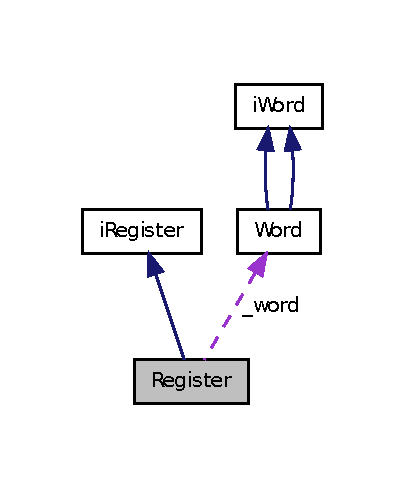
\includegraphics[width=197pt]{classRegister__coll__graph}
\end{center}
\end{figure}
\subsection*{Public Member Functions}
\begin{DoxyCompactItemize}
\item 
\hypertarget{classRegister_a73d8564754d7ddb7e8349001010e688b}{
void {\bfseries Add} (const \hyperlink{classiWord}{iWord} \&w)}
\label{classRegister_a73d8564754d7ddb7e8349001010e688b}

\item 
\hypertarget{classRegister_a9d9c6801db55e8706eb242b1e0e0fa3f}{
\hyperlink{classRegister}{Register} {\bfseries Add} (const \hyperlink{classiRegister}{iRegister} \&r) const }
\label{classRegister_a9d9c6801db55e8706eb242b1e0e0fa3f}

\item 
\hypertarget{classRegister_a312263efb06ef459409879f5119b3b81}{
void {\bfseries And} (const \hyperlink{classiWord}{iWord} \&w)}
\label{classRegister_a312263efb06ef459409879f5119b3b81}

\item 
\hypertarget{classRegister_af3502239502c214b8c9362a6fd9f8ff8}{
\hyperlink{classRegister}{Register} {\bfseries And} (const \hyperlink{classiRegister}{iRegister} \&r) const }
\label{classRegister_af3502239502c214b8c9362a6fd9f8ff8}

\item 
\hypertarget{classRegister_a379734c28ab8258ce528a96de24cfa1a}{
\hyperlink{classWord}{Word} {\bfseries GetValue} () const }
\label{classRegister_a379734c28ab8258ce528a96de24cfa1a}

\item 
\hypertarget{classRegister_abbf5f6793328db8b28845cac84c0e82d}{
void {\bfseries Not} ()}
\label{classRegister_abbf5f6793328db8b28845cac84c0e82d}

\item 
\hypertarget{classRegister_a387bb50d01b47071c366708ea10ebdf0}{
\hyperlink{classRegister}{Register} {\bfseries Not} () const }
\label{classRegister_a387bb50d01b47071c366708ea10ebdf0}

\item 
\hypertarget{classRegister_a55de0c3b5f8fe14df7c24bce777204e0}{
\hyperlink{classRegister}{Register} {\bfseries operator+} (const \hyperlink{classiRegister}{iRegister} \&r) const }
\label{classRegister_a55de0c3b5f8fe14df7c24bce777204e0}

\item 
\hypertarget{classRegister_ac4e78cff131bc5c69695a9db5ca35255}{
\hyperlink{classRegister}{Register} \& {\bfseries operator++} ()}
\label{classRegister_ac4e78cff131bc5c69695a9db5ca35255}

\item 
\hypertarget{classRegister_ae3414befdccf70a18df0f67dc19d86b7}{
\hyperlink{classRegister}{Register} \& {\bfseries operator++} (int)}
\label{classRegister_ae3414befdccf70a18df0f67dc19d86b7}

\item 
\hypertarget{classRegister_a43c957e4b6a3103f0634258891c82b46}{
\hyperlink{classRegister}{Register} {\bfseries operator-\/} (const \hyperlink{classiRegister}{iRegister} \&r) const }
\label{classRegister_a43c957e4b6a3103f0634258891c82b46}

\item 
\hypertarget{classRegister_afc5f775405700146638e392d81ad7d0b}{
\hyperlink{classRegister}{Register} \& {\bfseries operator=} (const \hyperlink{classiWord}{iWord} \&w)}
\label{classRegister_afc5f775405700146638e392d81ad7d0b}

\item 
\hypertarget{classRegister_a00f7aaf798102e5c7a6fb311551b492f}{
\hyperlink{classRegister}{Register} \& {\bfseries operator=} (const \hyperlink{classRegister}{Register} r)}
\label{classRegister_a00f7aaf798102e5c7a6fb311551b492f}

\item 
\hypertarget{classRegister_ab2f8407fab157d8deea936fa74424115}{
void {\bfseries Or} (const \hyperlink{classiWord}{iWord} \&w)}
\label{classRegister_ab2f8407fab157d8deea936fa74424115}

\item 
\hypertarget{classRegister_a9400801cc625144c4606cd7f5cbbaa21}{
\hyperlink{classRegister}{Register} {\bfseries Or} (const \hyperlink{classiRegister}{iRegister} \&r) const }
\label{classRegister_a9400801cc625144c4606cd7f5cbbaa21}

\item 
\hypertarget{classRegister_a6aea43b4c4ad669073f20fbcd274b49c}{
{\bfseries Register} (const \hyperlink{classWord}{Word} w)}
\label{classRegister_a6aea43b4c4ad669073f20fbcd274b49c}

\item 
\hypertarget{classRegister_affcc16cc88cdc896803b1ab6af5d38e0}{
void {\bfseries Store} (const \hyperlink{classiWord}{iWord} \&w)}
\label{classRegister_affcc16cc88cdc896803b1ab6af5d38e0}

\item 
\hypertarget{classRegister_a2ac7bd6f2e0eb38800c0a8c8d045e18e}{
void {\bfseries Store} (const \hyperlink{classiRegister}{iRegister} \&r)}
\label{classRegister_a2ac7bd6f2e0eb38800c0a8c8d045e18e}

\item 
\hypertarget{classRegister_a05132a4a62f5c6883fdf78731970ab6a}{
\hyperlink{classRegister}{Register} {\bfseries Subtract} (const \hyperlink{classiRegister}{iRegister} \&r) const }
\label{classRegister_a05132a4a62f5c6883fdf78731970ab6a}

\item 
\hypertarget{classRegister_a726a720b6bcca282945f1c0a65ca0dd4}{
void {\bfseries Subtract} (const \hyperlink{classiWord}{iWord} \&w)}
\label{classRegister_a726a720b6bcca282945f1c0a65ca0dd4}

\end{DoxyCompactItemize}
\subsection*{Private Attributes}
\begin{DoxyCompactItemize}
\item 
\hypertarget{classRegister_ad716faf568aba3da6e4acca6674f9ec9}{
\hyperlink{classWord}{Word} \hyperlink{classRegister_ad716faf568aba3da6e4acca6674f9ec9}{\_\-word}}
\label{classRegister_ad716faf568aba3da6e4acca6674f9ec9}

\begin{DoxyCompactList}\small\item\em The word of data held in the register. \item\end{DoxyCompactList}\end{DoxyCompactItemize}


\subsection{Detailed Description}
Implements \hyperlink{classiRegister}{iRegister}. 
\hypertarget{classResultDecoder}{
\section{ResultDecoder Class Reference}
\label{classResultDecoder}\index{ResultDecoder@{ResultDecoder}}
}


Finds the messages associated with a given result code.  


\subsection*{Public Member Functions}
\begin{DoxyCompactItemize}
\item 
std::string \hyperlink{classResultDecoder_ace7c2719b4f9de2a5e25fccfddc6d8f4}{Find} (const Codes::RESULT \&result) const 
\begin{DoxyCompactList}\small\item\em Looks up a result code. \item\end{DoxyCompactList}\item 
\hypertarget{classResultDecoder_afafd3458bdbcbd7b1b95545f47151358}{
\hyperlink{classResultDecoder_afafd3458bdbcbd7b1b95545f47151358}{ResultDecoder} ()}
\label{classResultDecoder_afafd3458bdbcbd7b1b95545f47151358}

\begin{DoxyCompactList}\small\item\em Generates the code-\/to-\/message mappings. \item\end{DoxyCompactList}\end{DoxyCompactItemize}
\subsection*{Static Private Attributes}
\begin{DoxyCompactItemize}
\item 
static std::map$<$ Codes::RESULT, std::string $>$ \hyperlink{classResultDecoder_ab19497e41c5d1a0546ed33642cad48dd}{\_\-codes}
\begin{DoxyCompactList}\small\item\em Maps a result code to, in every case but SUCCESS, an error message. \item\end{DoxyCompactList}\end{DoxyCompactItemize}


\subsection{Detailed Description}
Finds the messages associated with a given result code. 

\subsection{Member Function Documentation}
\hypertarget{classResultDecoder_ace7c2719b4f9de2a5e25fccfddc6d8f4}{
\index{ResultDecoder@{ResultDecoder}!Find@{Find}}
\index{Find@{Find}!ResultDecoder@{ResultDecoder}}
\subsubsection[{Find}]{\setlength{\rightskip}{0pt plus 5cm}std::string ResultDecoder::Find (
\begin{DoxyParamCaption}
\item[{const Codes::RESULT \&}]{ result}
\end{DoxyParamCaption}
) const}}
\label{classResultDecoder_ace7c2719b4f9de2a5e25fccfddc6d8f4}


Looks up a result code. 


\begin{DoxyParams}[1]{Parameters}
\mbox{\tt in}  & {\em result} & The result code to look up. \\
\hline
\end{DoxyParams}
\begin{DoxyReturn}{Returns}
The messages associated with \char`\"{}result\char`\"{}. 
\end{DoxyReturn}


\subsection{Member Data Documentation}
\hypertarget{classResultDecoder_ab19497e41c5d1a0546ed33642cad48dd}{
\index{ResultDecoder@{ResultDecoder}!\_\-codes@{\_\-codes}}
\index{\_\-codes@{\_\-codes}!ResultDecoder@{ResultDecoder}}
\subsubsection[{\_\-codes}]{\setlength{\rightskip}{0pt plus 5cm}std::map$<$Codes::RESULT, std::string$>$ {\bf ResultDecoder::\_\-codes}\hspace{0.3cm}{\ttfamily  \mbox{[}static, private\mbox{]}}}}
\label{classResultDecoder_ab19497e41c5d1a0546ed33642cad48dd}


Maps a result code to, in every case but SUCCESS, an error message. 

It is static because the result code messages should be available from anyhere. 
\hypertarget{classWi11}{
\section{Wi11 Class Reference}
\label{classWi11}\index{Wi11@{Wi11}}
}


Inheritance diagram for Wi11:
\nopagebreak
\begin{figure}[H]
\begin{center}
\leavevmode
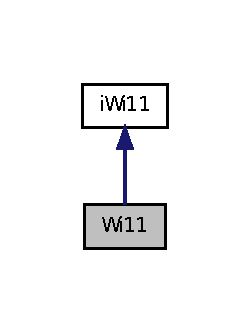
\includegraphics[width=120pt]{classWi11__inherit__graph}
\end{center}
\end{figure}


Collaboration diagram for Wi11:
\nopagebreak
\begin{figure}[H]
\begin{center}
\leavevmode
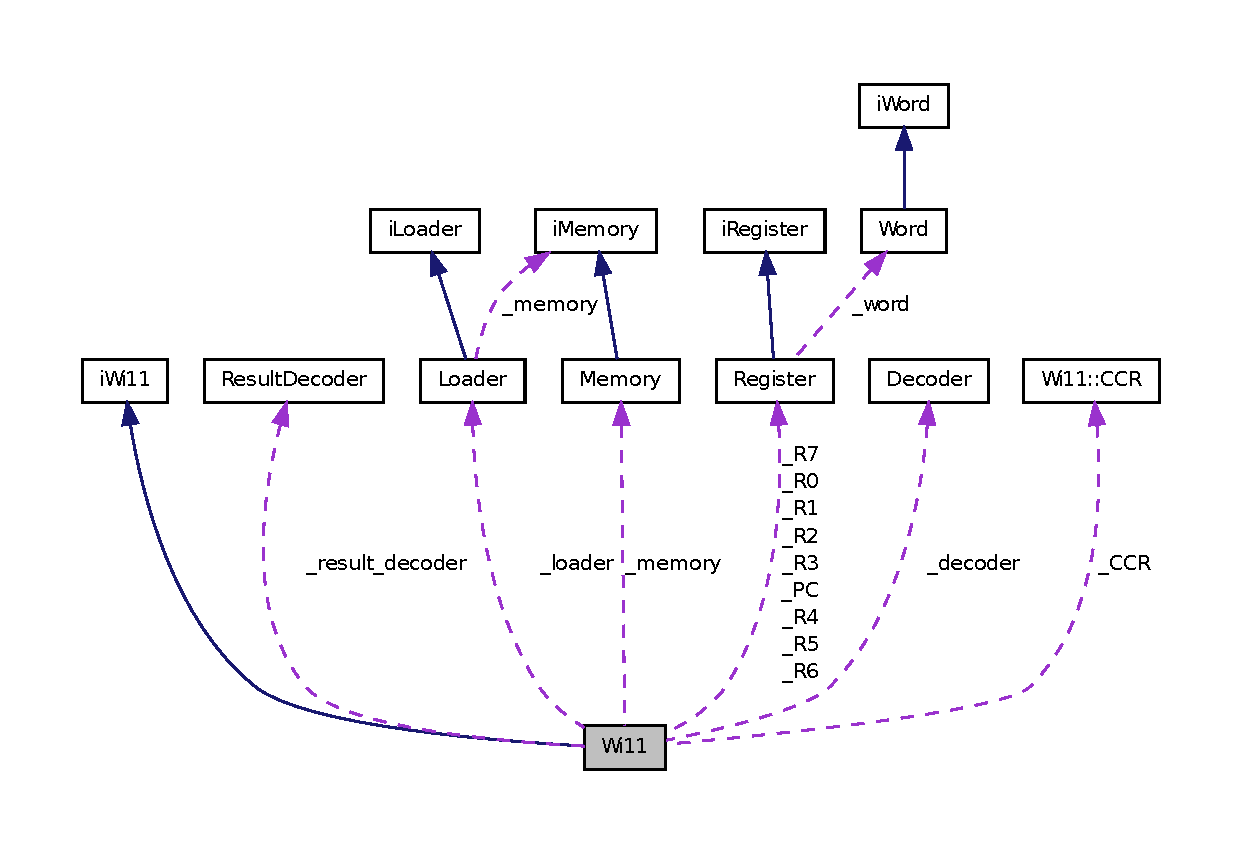
\includegraphics[width=273pt]{classWi11__coll__graph}
\end{center}
\end{figure}
\subsection*{Public Member Functions}
\begin{DoxyCompactItemize}
\item 
bool \hyperlink{classWi11_a1bd83a38f0ae1ff1436c98e73ff8b421}{LoadObj} (const char $\ast$filename)
\begin{DoxyCompactList}\small\item\em Loads the object file and sets up memory as it describes. \item\end{DoxyCompactList}\item 
void \hyperlink{classWi11_a0f532cefdebd3c33ddc93e8bce4dc06b}{DisplayMemory} () const 
\begin{DoxyCompactList}\small\item\em Prints the state of memory to standard out. \item\end{DoxyCompactList}\item 
void \hyperlink{classWi11_a201359b2506539dda72075b908076492}{DisplayRegisters} () const 
\begin{DoxyCompactList}\small\item\em Prints the state of every register to standard out. \item\end{DoxyCompactList}\item 
bool \hyperlink{classWi11_ace44826e4f92aabd233b68bdd9437c1b}{ExecuteNext} (bool verbose=false)
\begin{DoxyCompactList}\small\item\em Executes the instruction pointed to by the PC. \item\end{DoxyCompactList}\end{DoxyCompactItemize}
\subsection*{Private Member Functions}
\begin{DoxyCompactItemize}
\item 
\hyperlink{classiRegister}{iRegister} \& \hyperlink{classWi11_a17b5041499fa55f6b674e4f1ea8ceb59}{\_\-GetRegister} (const Decoder::REGISTER\_\-ID \&id)
\begin{DoxyCompactList}\small\item\em Retrieves a reference to the register corresponding to \char`\"{}id\char`\"{}. \item\end{DoxyCompactList}\item 
Codes::RESULT \hyperlink{classWi11_a818de966479e749f8592e73b35f5e2f2}{\_\-Add} (const Decoder::REGISTER\_\-ID DR, const Decoder::REGISTER\_\-ID SR1, const Decoder::REGISTER\_\-ID SR2)
\begin{DoxyCompactList}\small\item\em Adds two registers and stores the result in a third. \item\end{DoxyCompactList}\item 
Codes::RESULT \hyperlink{classWi11_ae3b47b19ae611cd4788891a812cc7ba0}{\_\-Add} (const Decoder::REGISTER\_\-ID DR, const Decoder::REGISTER\_\-ID SR1, const \hyperlink{classiWord}{iWord} \&immediate)
\begin{DoxyCompactList}\small\item\em Adds a constant to a register and stores the result in another. \item\end{DoxyCompactList}\item 
Codes::RESULT \hyperlink{classWi11_af1e68e7a15deeb829f1771855e108bc0}{\_\-And} (const Decoder::REGISTER\_\-ID DR, const Decoder::REGISTER\_\-ID SR1, const Decoder::REGISTER\_\-ID SR2)
\begin{DoxyCompactList}\small\item\em Bit-\/wise ands two registers and stores the result in a third. \item\end{DoxyCompactList}\item 
Codes::RESULT \hyperlink{classWi11_abb98c230c0e384e4d3a3b9f0e3606db4}{\_\-And} (const Decoder::REGISTER\_\-ID DR, const Decoder::REGISTER\_\-ID SR1, const \hyperlink{classiWord}{iWord} \&immediate)
\begin{DoxyCompactList}\small\item\em Bit-\/wise ands a register with a constant and stores the result in another register. \item\end{DoxyCompactList}\item 
Codes::RESULT \hyperlink{classWi11_a09edab9ea53d62c93d5d42bfaa77adf5}{\_\-Branch} (const \hyperlink{classiWord}{iWord} \&address)
\begin{DoxyCompactList}\small\item\em Changes the last 9 bits of the PC. \item\end{DoxyCompactList}\item 
Codes::RESULT \hyperlink{classWi11_a08581ef7b0fa3939185ffa516c905d65}{\_\-Debug} ()
\begin{DoxyCompactList}\small\item\em Deprecated? \item\end{DoxyCompactList}\item 
Codes::RESULT \hyperlink{classWi11_a84b28efa218ee676a4482e38069f5f8b}{\_\-JSR} (const \hyperlink{classiWord}{iWord} \&w)
\begin{DoxyCompactList}\small\item\em Initiate a jump to a subroutine (alter the PC). \item\end{DoxyCompactList}\item 
Codes::RESULT \hyperlink{classWi11_a884c75a5dbe753bc316fb2a8faa30e56}{\_\-JSRR} (const \hyperlink{classiWord}{iWord} \&baseR, const \hyperlink{classiWord}{iWord} \&address)
\begin{DoxyCompactList}\small\item\em Initiate a jump to a subroutine (alter the PC). param\mbox{[}in\mbox{]} baseR A register whose value acts as a base address. \item\end{DoxyCompactList}\item 
Codes::RESULT \hyperlink{classWi11_a521c4d4d670b8bb1e1e7e9226ec2f259}{\_\-Load} (const Decoder::REGISTER\_\-ID DR, const \hyperlink{classiWord}{iWord} \&address)
\begin{DoxyCompactList}\small\item\em Loads a word in memory into a register. \item\end{DoxyCompactList}\item 
Codes::RESULT \hyperlink{classWi11_a76e05be82843d69572d1b3c9a84f4eb0}{\_\-LoadI} (const Decoder::REGISTER\_\-ID DR, const \hyperlink{classiWord}{iWord} \&address)
\begin{DoxyCompactList}\small\item\em Performs an indirect load. \item\end{DoxyCompactList}\item 
Codes::RESULT \hyperlink{classWi11_a58c642a908084d7629c93e702558e05a}{\_\-LoadR} (const Decoder::REGISTER\_\-ID DR, Decoder::REGISTER\_\-ID baseR, const \hyperlink{classiWord}{iWord} \&address)
\begin{DoxyCompactList}\small\item\em Performs a register-\/relative load. \item\end{DoxyCompactList}\item 
Codes::RESULT \hyperlink{classWi11_a13742e76d8e61aa08696459f5bdcaddb}{\_\-Not} (const Decoder::REGISTER\_\-ID DR, const Decoder::REGISTER\_\-ID SR)
\begin{DoxyCompactList}\small\item\em Bit-\/wise nots a register and stores the result in another. \item\end{DoxyCompactList}\item 
Codes::RESULT \hyperlink{classWi11_ad49e98e49ec62664b3684d63568545f0}{\_\-Ret} ()
\begin{DoxyCompactList}\small\item\em Return from a subroutine. \item\end{DoxyCompactList}\item 
Codes::RESULT \hyperlink{classWi11_a35746dfc067eedf054ade3c6aeb13eca}{\_\-Store} (const Decoder::REGISTER\_\-ID SR1, const \hyperlink{classiWord}{iWord} \&address)
\begin{DoxyCompactList}\small\item\em Stores a register's value into memory at a specified address. \item\end{DoxyCompactList}\item 
Codes::RESULT \hyperlink{classWi11_a7b360f2afbe98cd267941d0a8c584260}{\_\-STI} (const Decoder::REGISTER\_\-ID SR1, const \hyperlink{classiWord}{iWord} \&address)
\begin{DoxyCompactList}\small\item\em Performs an indirect store. \item\end{DoxyCompactList}\item 
Codes::RESULT \hyperlink{classWi11_a43d17c3207c05f5519336ff9c2974b2d}{\_\-STR} (const Decoder::REGISTER\_\-ID SR1, const Decoder::REGISTER\_\-ID baseR, const \hyperlink{classiWord}{iWord} \&address)
\begin{DoxyCompactList}\small\item\em Perfroms a register-\/relative store. \item\end{DoxyCompactList}\item 
Codes::RESULT \hyperlink{classWi11_af981c1237ba25082ecd7aee3820d19e3}{\_\-Trap} (const \hyperlink{classiWord}{iWord} \&code)
\begin{DoxyCompactList}\small\item\em Branches to a trap vector. \item\end{DoxyCompactList}\end{DoxyCompactItemize}
\subsection*{Private Attributes}
\begin{DoxyCompactItemize}
\item 
\hypertarget{classWi11_a4eb624a34718b061c5d1a9704e1511cb}{
\hyperlink{classMemory}{Memory} \hyperlink{classWi11_a4eb624a34718b061c5d1a9704e1511cb}{\_\-mem}}
\label{classWi11_a4eb624a34718b061c5d1a9704e1511cb}

\begin{DoxyCompactList}\small\item\em Wi-\/11's memory. \item\end{DoxyCompactList}\item 
\hypertarget{classWi11_a5db0201cfce46192ffa48e0e7d8661c2}{
\hyperlink{classRegister}{Register} \hyperlink{classWi11_a5db0201cfce46192ffa48e0e7d8661c2}{\_\-reg} \mbox{[}8\mbox{]}}
\label{classWi11_a5db0201cfce46192ffa48e0e7d8661c2}

\begin{DoxyCompactList}\small\item\em 8 general purpose registers. \item\end{DoxyCompactList}\item 
\hypertarget{classWi11_a78b431105c8d82444b3c94401e0e0977}{
bool \hyperlink{classWi11_a78b431105c8d82444b3c94401e0e0977}{\_\-pos}}
\label{classWi11_a78b431105c8d82444b3c94401e0e0977}

\begin{DoxyCompactList}\small\item\em CCR, true iff positive. \item\end{DoxyCompactList}\item 
\hypertarget{classWi11_a2d23fc7d842995772d7f3280f900ca4a}{
bool \hyperlink{classWi11_a2d23fc7d842995772d7f3280f900ca4a}{\_\-zero}}
\label{classWi11_a2d23fc7d842995772d7f3280f900ca4a}

\begin{DoxyCompactList}\small\item\em CCR, true iff zero. \item\end{DoxyCompactList}\end{DoxyCompactItemize}


\subsection{Member Function Documentation}
\hypertarget{classWi11_a17b5041499fa55f6b674e4f1ea8ceb59}{
\index{Wi11@{Wi11}!\_\-GetRegister@{\_\-GetRegister}}
\index{\_\-GetRegister@{\_\-GetRegister}!Wi11@{Wi11}}
\subsubsection[{\_\-GetRegister}]{\setlength{\rightskip}{0pt plus 5cm}{\bf iRegister}\& Wi11::\_\-GetRegister (
\begin{DoxyParamCaption}
\item[{const Decoder::REGISTER\_\-ID \&}]{ id}
\end{DoxyParamCaption}
)\hspace{0.3cm}{\ttfamily  \mbox{[}private, virtual\mbox{]}}}}
\label{classWi11_a17b5041499fa55f6b674e4f1ea8ceb59}


Retrieves a reference to the register corresponding to \char`\"{}id\char`\"{}. 


\begin{DoxyParams}[1]{Parameters}
\mbox{\tt in}  & {\em id} & A REGISTER\_\-ID corresponding to one of the private registers. \\
\hline
\end{DoxyParams}
\begin{DoxyReturn}{Returns}
A reference to the id'd register. 
\end{DoxyReturn}


Implements \hyperlink{classiWi11_aa1696b5bb260a94e1fb4a9922369cebf}{iWi11}.

\hypertarget{classWi11_a818de966479e749f8592e73b35f5e2f2}{
\index{Wi11@{Wi11}!\_\-Add@{\_\-Add}}
\index{\_\-Add@{\_\-Add}!Wi11@{Wi11}}
\subsubsection[{\_\-Add}]{\setlength{\rightskip}{0pt plus 5cm}Codes::RESULT Wi11::\_\-Add (
\begin{DoxyParamCaption}
\item[{const Decoder::REGISTER\_\-ID}]{ DR, }
\item[{const Decoder::REGISTER\_\-ID}]{ SR1, }
\item[{const Decoder::REGISTER\_\-ID}]{ SR2}
\end{DoxyParamCaption}
)\hspace{0.3cm}{\ttfamily  \mbox{[}private, virtual\mbox{]}}}}
\label{classWi11_a818de966479e749f8592e73b35f5e2f2}


Adds two registers and stores the result in a third. 


\begin{DoxyParams}[1]{Parameters}
\mbox{\tt out}  & {\em DR} & The destination register. \\
\hline
\mbox{\tt in}  & {\em SR1} & The first source register. \\
\hline
\mbox{\tt in}  & {\em SR2} & The second source register. \\
\hline
\end{DoxyParams}
\begin{DoxyPostcond}{Postcondition}
SR1 and SR2 are not changed. 
\end{DoxyPostcond}
\begin{DoxyReturn}{Returns}
SUCCESS or, if something went wrong, an appropriate error code.
\end{DoxyReturn}
\begin{DoxyNote}{Note}
Updates the CCR. 
\end{DoxyNote}


Implements \hyperlink{classiWi11_a65f699c773084a631cd7373cae05b5da}{iWi11}.

\hypertarget{classWi11_ae3b47b19ae611cd4788891a812cc7ba0}{
\index{Wi11@{Wi11}!\_\-Add@{\_\-Add}}
\index{\_\-Add@{\_\-Add}!Wi11@{Wi11}}
\subsubsection[{\_\-Add}]{\setlength{\rightskip}{0pt plus 5cm}Codes::RESULT Wi11::\_\-Add (
\begin{DoxyParamCaption}
\item[{const Decoder::REGISTER\_\-ID}]{ DR, }
\item[{const Decoder::REGISTER\_\-ID}]{ SR1, }
\item[{const {\bf iWord} \&}]{ immediate}
\end{DoxyParamCaption}
)\hspace{0.3cm}{\ttfamily  \mbox{[}private, virtual\mbox{]}}}}
\label{classWi11_ae3b47b19ae611cd4788891a812cc7ba0}


Adds a constant to a register and stores the result in another. 


\begin{DoxyParams}[1]{Parameters}
\mbox{\tt out}  & {\em DR} & The destination register. \\
\hline
\mbox{\tt in}  & {\em SR1} & The source register. \\
\hline
\mbox{\tt in}  & {\em immediate} & The immediate value. \\
\hline
\end{DoxyParams}
\begin{DoxyPostcond}{Postcondition}
SR1 and \char`\"{}immediate\char`\"{} are not changed. 
\end{DoxyPostcond}
\begin{DoxyReturn}{Returns}
SUCCESS or, if something went wrong, an appropriate error code.
\end{DoxyReturn}
\begin{DoxyNote}{Note}
Updates the CCR. 
\end{DoxyNote}


Implements \hyperlink{classiWi11_a6345dc089e3a699bd30fc442bd8f6d85}{iWi11}.

\hypertarget{classWi11_af1e68e7a15deeb829f1771855e108bc0}{
\index{Wi11@{Wi11}!\_\-And@{\_\-And}}
\index{\_\-And@{\_\-And}!Wi11@{Wi11}}
\subsubsection[{\_\-And}]{\setlength{\rightskip}{0pt plus 5cm}Codes::RESULT Wi11::\_\-And (
\begin{DoxyParamCaption}
\item[{const Decoder::REGISTER\_\-ID}]{ DR, }
\item[{const Decoder::REGISTER\_\-ID}]{ SR1, }
\item[{const Decoder::REGISTER\_\-ID}]{ SR2}
\end{DoxyParamCaption}
)\hspace{0.3cm}{\ttfamily  \mbox{[}private, virtual\mbox{]}}}}
\label{classWi11_af1e68e7a15deeb829f1771855e108bc0}


Bit-\/wise ands two registers and stores the result in a third. 


\begin{DoxyParams}[1]{Parameters}
\mbox{\tt out}  & {\em DR} & The destination register. \\
\hline
\mbox{\tt in}  & {\em SR1} & The first source register. \\
\hline
\mbox{\tt in}  & {\em SR2} & The second source register. \\
\hline
\end{DoxyParams}
\begin{DoxyPostcond}{Postcondition}
SR1 and SR2 are not changed. 
\end{DoxyPostcond}
\begin{DoxyReturn}{Returns}
SUCCESS or, if something went wrong, an appropriate error code.
\end{DoxyReturn}
\begin{DoxyNote}{Note}
Updates the CCR. 
\end{DoxyNote}


Implements \hyperlink{classiWi11_a90cd8f3daa1788f029cabe198c19efb3}{iWi11}.

\hypertarget{classWi11_abb98c230c0e384e4d3a3b9f0e3606db4}{
\index{Wi11@{Wi11}!\_\-And@{\_\-And}}
\index{\_\-And@{\_\-And}!Wi11@{Wi11}}
\subsubsection[{\_\-And}]{\setlength{\rightskip}{0pt plus 5cm}Codes::RESULT Wi11::\_\-And (
\begin{DoxyParamCaption}
\item[{const Decoder::REGISTER\_\-ID}]{ DR, }
\item[{const Decoder::REGISTER\_\-ID}]{ SR1, }
\item[{const {\bf iWord} \&}]{ immediate}
\end{DoxyParamCaption}
)\hspace{0.3cm}{\ttfamily  \mbox{[}private, virtual\mbox{]}}}}
\label{classWi11_abb98c230c0e384e4d3a3b9f0e3606db4}


Bit-\/wise ands a register with a constant and stores the result in another register. 


\begin{DoxyParams}[1]{Parameters}
\mbox{\tt out}  & {\em DR} & The destination register. \\
\hline
\mbox{\tt in}  & {\em SR1} & The source register. \\
\hline
\mbox{\tt in}  & {\em immediate} & The immediate value. \\
\hline
\end{DoxyParams}
\begin{DoxyPostcond}{Postcondition}
SR1 and \char`\"{}immediate\char`\"{} are not changed. 
\end{DoxyPostcond}
\begin{DoxyReturn}{Returns}
SUCCESS or, if something went wrong, an appropriate error code.
\end{DoxyReturn}
\begin{DoxyNote}{Note}
Updates the CCR. 
\end{DoxyNote}


Implements \hyperlink{classiWi11_a4785e197f77fb0861e97e8d18c3be96f}{iWi11}.

\hypertarget{classWi11_a09edab9ea53d62c93d5d42bfaa77adf5}{
\index{Wi11@{Wi11}!\_\-Branch@{\_\-Branch}}
\index{\_\-Branch@{\_\-Branch}!Wi11@{Wi11}}
\subsubsection[{\_\-Branch}]{\setlength{\rightskip}{0pt plus 5cm}Codes::RESULT Wi11::\_\-Branch (
\begin{DoxyParamCaption}
\item[{const {\bf iWord} \&}]{ address}
\end{DoxyParamCaption}
)\hspace{0.3cm}{\ttfamily  \mbox{[}private, virtual\mbox{]}}}}
\label{classWi11_a09edab9ea53d62c93d5d42bfaa77adf5}


Changes the last 9 bits of the PC. 


\begin{DoxyParams}[1]{Parameters}
\mbox{\tt in}  & {\em address} & The 9 bits to become the end of the PC. \\
\hline
\end{DoxyParams}
\begin{DoxyPostcond}{Postcondition}
\char`\"{}address\char`\"{} is not changed. 
\end{DoxyPostcond}
\begin{DoxyReturn}{Returns}
SUCCESS or, if something went wrong, an appropriate error code. 
\end{DoxyReturn}


Implements \hyperlink{classiWi11_a42d2c50609424634873413d7a6614397}{iWi11}.

\hypertarget{classWi11_a08581ef7b0fa3939185ffa516c905d65}{
\index{Wi11@{Wi11}!\_\-Debug@{\_\-Debug}}
\index{\_\-Debug@{\_\-Debug}!Wi11@{Wi11}}
\subsubsection[{\_\-Debug}]{\setlength{\rightskip}{0pt plus 5cm}Codes::RESULT Wi11::\_\-Debug (
\begin{DoxyParamCaption}
{}
\end{DoxyParamCaption}
)\hspace{0.3cm}{\ttfamily  \mbox{[}private, virtual\mbox{]}}}}
\label{classWi11_a08581ef7b0fa3939185ffa516c905d65}


Deprecated? 

Does nothing. 

Implements \hyperlink{classiWi11_ae510f127a0c3b87d42cdbe5b14204a65}{iWi11}.

\hypertarget{classWi11_a84b28efa218ee676a4482e38069f5f8b}{
\index{Wi11@{Wi11}!\_\-JSR@{\_\-JSR}}
\index{\_\-JSR@{\_\-JSR}!Wi11@{Wi11}}
\subsubsection[{\_\-JSR}]{\setlength{\rightskip}{0pt plus 5cm}Codes::RESULT Wi11::\_\-JSR (
\begin{DoxyParamCaption}
\item[{const {\bf iWord} \&}]{ w}
\end{DoxyParamCaption}
)\hspace{0.3cm}{\ttfamily  \mbox{[}private, virtual\mbox{]}}}}
\label{classWi11_a84b28efa218ee676a4482e38069f5f8b}


Initiate a jump to a subroutine (alter the PC). 


\begin{DoxyParams}[1]{Parameters}
\mbox{\tt in}  & {\em w} & A 9 bit offset for the PC. \\
\hline
\end{DoxyParams}
\begin{DoxyPostcond}{Postcondition}
The PC has \char`\"{}w\char`\"{} as its 9 least significant bits. 
\end{DoxyPostcond}
\begin{DoxyReturn}{Returns}
SUCCESS or, if something went wrong, an appropriate error code.
\end{DoxyReturn}
\begin{DoxyNote}{Note}
If the link bit was set for this instruction, R7 will hold the old value of the PC. However, the CCR will not be altered for this instruction, depite R7 being altered. 
\end{DoxyNote}


Implements \hyperlink{classiWi11_ace280c40256d3e0c575b08cf6a0d36f5}{iWi11}.

\hypertarget{classWi11_a884c75a5dbe753bc316fb2a8faa30e56}{
\index{Wi11@{Wi11}!\_\-JSRR@{\_\-JSRR}}
\index{\_\-JSRR@{\_\-JSRR}!Wi11@{Wi11}}
\subsubsection[{\_\-JSRR}]{\setlength{\rightskip}{0pt plus 5cm}Codes::RESULT Wi11::\_\-JSRR (
\begin{DoxyParamCaption}
\item[{const {\bf iWord} \&}]{ baseR, }
\item[{const {\bf iWord} \&}]{ address}
\end{DoxyParamCaption}
)\hspace{0.3cm}{\ttfamily  \mbox{[}private, virtual\mbox{]}}}}
\label{classWi11_a884c75a5dbe753bc316fb2a8faa30e56}


Initiate a jump to a subroutine (alter the PC). param\mbox{[}in\mbox{]} baseR A register whose value acts as a base address. 


\begin{DoxyParams}[1]{Parameters}
\mbox{\tt in}  & {\em address} & A 6 bit offset to the base address. \\
\hline
\end{DoxyParams}
\begin{DoxyPostcond}{Postcondition}
The PC is the value in baseR plus the value in address. 
\end{DoxyPostcond}
\begin{DoxyReturn}{Returns}
SUCCESS or, if something went wrong, an appropriate error code.
\end{DoxyReturn}
\begin{DoxyNote}{Note}
If the link bit was set for this instruction, R7 will hold the old value of the PC. However, the CCR will not be altered for this instruction, depite R7 being altered. 
\end{DoxyNote}


Implements \hyperlink{classiWi11_aeabd561f2728e2345b6a5ae5cdd5b84a}{iWi11}.

\hypertarget{classWi11_a521c4d4d670b8bb1e1e7e9226ec2f259}{
\index{Wi11@{Wi11}!\_\-Load@{\_\-Load}}
\index{\_\-Load@{\_\-Load}!Wi11@{Wi11}}
\subsubsection[{\_\-Load}]{\setlength{\rightskip}{0pt plus 5cm}Codes::RESULT Wi11::\_\-Load (
\begin{DoxyParamCaption}
\item[{const Decoder::REGISTER\_\-ID}]{ DR, }
\item[{const {\bf iWord} \&}]{ address}
\end{DoxyParamCaption}
)\hspace{0.3cm}{\ttfamily  \mbox{[}private, virtual\mbox{]}}}}
\label{classWi11_a521c4d4d670b8bb1e1e7e9226ec2f259}


Loads a word in memory into a register. 


\begin{DoxyParams}[1]{Parameters}
\mbox{\tt out}  & {\em DR} & The destination register. \\
\hline
\mbox{\tt in}  & {\em address} & When concatenated with the PC, forms address in memory from which to load. \\
\hline
\end{DoxyParams}
\begin{DoxyPostcond}{Postcondition}
\hyperlink{classMemory}{Memory} and \char`\"{}address\char`\"{} have not changed. 
\end{DoxyPostcond}
\begin{DoxyReturn}{Returns}
SUCCESS or, if something went wrong, an appropriate error code.
\end{DoxyReturn}
\begin{DoxyNote}{Note}
Updates the CCR. 
\end{DoxyNote}


Implements \hyperlink{classiWi11_aed1f870b129617436434bb6dcee521ce}{iWi11}.

\hypertarget{classWi11_a76e05be82843d69572d1b3c9a84f4eb0}{
\index{Wi11@{Wi11}!\_\-LoadI@{\_\-LoadI}}
\index{\_\-LoadI@{\_\-LoadI}!Wi11@{Wi11}}
\subsubsection[{\_\-LoadI}]{\setlength{\rightskip}{0pt plus 5cm}Codes::RESULT Wi11::\_\-LoadI (
\begin{DoxyParamCaption}
\item[{const Decoder::REGISTER\_\-ID}]{ DR, }
\item[{const {\bf iWord} \&}]{ address}
\end{DoxyParamCaption}
)\hspace{0.3cm}{\ttfamily  \mbox{[}private, virtual\mbox{]}}}}
\label{classWi11_a76e05be82843d69572d1b3c9a84f4eb0}


Performs an indirect load. 


\begin{DoxyParams}[1]{Parameters}
\mbox{\tt out}  & {\em DR} & The destination register. \\
\hline
\mbox{\tt in}  & {\em address} & A 9-\/bit offset to the PC. \\
\hline
\end{DoxyParams}
\begin{DoxyPostcond}{Postcondition}
\hyperlink{classMemory}{Memory} and \char`\"{}address\char`\"{} have not changed. 
\end{DoxyPostcond}
\begin{DoxyReturn}{Returns}
SUCCESS or, if something went wrong, an appropriate error code.
\end{DoxyReturn}
Works similar to \_\-Load() but when memory is read, it uses the address found to again access memory. In this indirect way, a load can be made from anywhere in \hyperlink{classMemory}{Memory}.

\begin{DoxyNote}{Note}
Updates the CCR. 
\end{DoxyNote}


Implements \hyperlink{classiWi11_ab8f6fc32bfc363f9798c795320c00894}{iWi11}.

\hypertarget{classWi11_a58c642a908084d7629c93e702558e05a}{
\index{Wi11@{Wi11}!\_\-LoadR@{\_\-LoadR}}
\index{\_\-LoadR@{\_\-LoadR}!Wi11@{Wi11}}
\subsubsection[{\_\-LoadR}]{\setlength{\rightskip}{0pt plus 5cm}Codes::RESULT Wi11::\_\-LoadR (
\begin{DoxyParamCaption}
\item[{const Decoder::REGISTER\_\-ID}]{ DR, }
\item[{Decoder::REGISTER\_\-ID}]{ baseR, }
\item[{const {\bf iWord} \&}]{ address}
\end{DoxyParamCaption}
)\hspace{0.3cm}{\ttfamily  \mbox{[}private, virtual\mbox{]}}}}
\label{classWi11_a58c642a908084d7629c93e702558e05a}


Performs a register-\/relative load. 


\begin{DoxyParams}[1]{Parameters}
\mbox{\tt out}  & {\em DR} & The destination register. \\
\hline
\mbox{\tt in}  & {\em baseR} & A register whose value works as a base address. \\
\hline
\mbox{\tt in}  & {\em address} & An 6-\/bit index from the base address. \\
\hline
\end{DoxyParams}
\begin{DoxyPostcond}{Postcondition}
\hyperlink{classMemory}{Memory}, \char`\"{}baseR\char`\"{}, and \char`\"{}address\char`\"{} have no changed. 
\end{DoxyPostcond}
\begin{DoxyReturn}{Returns}
SUCCESS or, if something went wrong, an appropriate error code.
\end{DoxyReturn}
Loads from \char`\"{}baseR\char`\"{} plus \char`\"{}address\char`\"{}.

\begin{DoxyNote}{Note}
Updates the CCR. 
\end{DoxyNote}


Implements \hyperlink{classiWi11_a47fd64cc3629f9239c75fa4fea753c41}{iWi11}.

\hypertarget{classWi11_a13742e76d8e61aa08696459f5bdcaddb}{
\index{Wi11@{Wi11}!\_\-Not@{\_\-Not}}
\index{\_\-Not@{\_\-Not}!Wi11@{Wi11}}
\subsubsection[{\_\-Not}]{\setlength{\rightskip}{0pt plus 5cm}Codes::RESULT Wi11::\_\-Not (
\begin{DoxyParamCaption}
\item[{const Decoder::REGISTER\_\-ID}]{ DR, }
\item[{const Decoder::REGISTER\_\-ID}]{ SR}
\end{DoxyParamCaption}
)\hspace{0.3cm}{\ttfamily  \mbox{[}private, virtual\mbox{]}}}}
\label{classWi11_a13742e76d8e61aa08696459f5bdcaddb}


Bit-\/wise nots a register and stores the result in another. 


\begin{DoxyParams}[1]{Parameters}
\mbox{\tt out}  & {\em DR} & The destination register. \\
\hline
\mbox{\tt in}  & {\em SR} & The source register. \\
\hline
\end{DoxyParams}
\begin{DoxyReturn}{Returns}
SUCCESS or, if something went wrong, an appropriate error code.
\end{DoxyReturn}
\begin{DoxyNote}{Note}
Updates the CCR. 
\end{DoxyNote}


Implements \hyperlink{classiWi11_a942ecd7956af6ad9c65c976b968d7832}{iWi11}.

\hypertarget{classWi11_ad49e98e49ec62664b3684d63568545f0}{
\index{Wi11@{Wi11}!\_\-Ret@{\_\-Ret}}
\index{\_\-Ret@{\_\-Ret}!Wi11@{Wi11}}
\subsubsection[{\_\-Ret}]{\setlength{\rightskip}{0pt plus 5cm}Codes::RESULT Wi11::\_\-Ret (
\begin{DoxyParamCaption}
{}
\end{DoxyParamCaption}
)\hspace{0.3cm}{\ttfamily  \mbox{[}private, virtual\mbox{]}}}}
\label{classWi11_ad49e98e49ec62664b3684d63568545f0}


Return from a subroutine. 

\begin{DoxyPostcond}{Postcondition}
The PC now holds the value that was (and still is) in R7. 
\end{DoxyPostcond}
\begin{DoxyReturn}{Returns}
SUCCESS or, if something went wrong, an appropriate error code.
\end{DoxyReturn}
\begin{DoxyNote}{Note}

\end{DoxyNote}
\begin{DoxyParagraph}{}
This can be used to jump anywhere in memory. However, this is not the intended usage. 
\end{DoxyParagraph}
\begin{DoxyParagraph}{}
Updates the CCR. 
\end{DoxyParagraph}


Implements \hyperlink{classiWi11_ae6c1048642dbf2c03c60062f6aaabfd2}{iWi11}.

\hypertarget{classWi11_a35746dfc067eedf054ade3c6aeb13eca}{
\index{Wi11@{Wi11}!\_\-Store@{\_\-Store}}
\index{\_\-Store@{\_\-Store}!Wi11@{Wi11}}
\subsubsection[{\_\-Store}]{\setlength{\rightskip}{0pt plus 5cm}Codes::RESULT Wi11::\_\-Store (
\begin{DoxyParamCaption}
\item[{const Decoder::REGISTER\_\-ID}]{ SR1, }
\item[{const {\bf iWord} \&}]{ address}
\end{DoxyParamCaption}
)\hspace{0.3cm}{\ttfamily  \mbox{[}private, virtual\mbox{]}}}}
\label{classWi11_a35746dfc067eedf054ade3c6aeb13eca}


Stores a register's value into memory at a specified address. 


\begin{DoxyParams}[1]{Parameters}
\mbox{\tt in}  & {\em SR1} & The source register (holds the data to be stored). \\
\hline
\mbox{\tt in}  & {\em address} & When concatenated with the PC, forms the address for the store. \\
\hline
\end{DoxyParams}
\begin{DoxyPostcond}{Postcondition}
SR1 and \char`\"{}address\char`\"{} are not changed. 
\end{DoxyPostcond}
\begin{DoxyReturn}{Returns}
SUCCESS or, if something went wrong, an appropriate error code. 
\end{DoxyReturn}


Implements \hyperlink{classiWi11_a52659070aca67bf8fba76f059bc120aa}{iWi11}.

\hypertarget{classWi11_a7b360f2afbe98cd267941d0a8c584260}{
\index{Wi11@{Wi11}!\_\-STI@{\_\-STI}}
\index{\_\-STI@{\_\-STI}!Wi11@{Wi11}}
\subsubsection[{\_\-STI}]{\setlength{\rightskip}{0pt plus 5cm}Codes::RESULT Wi11::\_\-STI (
\begin{DoxyParamCaption}
\item[{const Decoder::REGISTER\_\-ID}]{ SR1, }
\item[{const {\bf iWord} \&}]{ address}
\end{DoxyParamCaption}
)\hspace{0.3cm}{\ttfamily  \mbox{[}private, virtual\mbox{]}}}}
\label{classWi11_a7b360f2afbe98cd267941d0a8c584260}


Performs an indirect store. 


\begin{DoxyParams}[1]{Parameters}
\mbox{\tt in}  & {\em SR1} & The source register (holds the data to be stored). \\
\hline
\mbox{\tt in}  & {\em address} & A 9-\/bit offset to the PC. \\
\hline
\end{DoxyParams}
\begin{DoxyPostcond}{Postcondition}
\char`\"{}SR1\char`\"{} and \char`\"{}address\char`\"{} are not changed. 
\end{DoxyPostcond}
\begin{DoxyReturn}{Returns}
SUCCESS or, if something went wrong, an appropriate error code.
\end{DoxyReturn}
Works similar to \_\-Store() but when memory is read, it uses the address found to again access memory. In this indirect way, a store can be made to anywhere in \hyperlink{classMemory}{Memory}. 

Implements \hyperlink{classiWi11_a3a299e4526c8c9865f529cc10e293a0c}{iWi11}.

\hypertarget{classWi11_a43d17c3207c05f5519336ff9c2974b2d}{
\index{Wi11@{Wi11}!\_\-STR@{\_\-STR}}
\index{\_\-STR@{\_\-STR}!Wi11@{Wi11}}
\subsubsection[{\_\-STR}]{\setlength{\rightskip}{0pt plus 5cm}Codes::RESULT Wi11::\_\-STR (
\begin{DoxyParamCaption}
\item[{const Decoder::REGISTER\_\-ID}]{ SR1, }
\item[{const Decoder::REGISTER\_\-ID}]{ baseR, }
\item[{const {\bf iWord} \&}]{ address}
\end{DoxyParamCaption}
)\hspace{0.3cm}{\ttfamily  \mbox{[}private, virtual\mbox{]}}}}
\label{classWi11_a43d17c3207c05f5519336ff9c2974b2d}


Perfroms a register-\/relative store. 


\begin{DoxyParams}[1]{Parameters}
\mbox{\tt in}  & {\em SR1} & The source register (holds the data to be stored). \\
\hline
\mbox{\tt in}  & {\em baseR} & A register whose value acts as a base address. \\
\hline
\mbox{\tt in}  & {\em address} & A 6-\/bit index from the base address. \\
\hline
\end{DoxyParams}
\begin{DoxyPostcond}{Postcondition}
SR1, baseR, and \char`\"{}address\char`\"{} are not changed. 
\end{DoxyPostcond}
\begin{DoxyReturn}{Returns}
SUCCESS or, if something went wrong, an appropriate error code. 
\end{DoxyReturn}


Implements \hyperlink{classiWi11_a5002f010e61f0677feb9f8a116504a0c}{iWi11}.

\hypertarget{classWi11_af981c1237ba25082ecd7aee3820d19e3}{
\index{Wi11@{Wi11}!\_\-Trap@{\_\-Trap}}
\index{\_\-Trap@{\_\-Trap}!Wi11@{Wi11}}
\subsubsection[{\_\-Trap}]{\setlength{\rightskip}{0pt plus 5cm}Codes::RESULT Wi11::\_\-Trap (
\begin{DoxyParamCaption}
\item[{const {\bf iWord} \&}]{ code}
\end{DoxyParamCaption}
)\hspace{0.3cm}{\ttfamily  \mbox{[}private, virtual\mbox{]}}}}
\label{classWi11_af981c1237ba25082ecd7aee3820d19e3}


Branches to a trap vector. 


\begin{DoxyParams}[1]{Parameters}
\mbox{\tt in}  & {\em code} & The trap code. \\
\hline
\end{DoxyParams}
\begin{DoxyPostcond}{Postcondition}
\char`\"{}code\char`\"{} is not changed. 
\end{DoxyPostcond}
\begin{DoxyReturn}{Returns}
SUCCESS or, if something went wrong, an appropriate error code.
\end{DoxyReturn}
\begin{DoxyParagraph}{}
The traps are as follows: \begin{DoxyItemize}
\item 0x21 -\/ OUT -\/ Write the character formed from the eight least significant bits of R0 to standard out. \item 0x22 -\/ PUTS -\/ Write the a string to standard out starting at the address pointed to by R0 and ending at a null character. \item 0x23 -\/ IN -\/ Prompt for, and read, a single character from standard in. Re-\/print it and store its ascii value in R0 (with leading zeros). \item 0x25 -\/ HALT -\/ End execution and print an appropriate message to standard out. \item 0x31 -\/ INN -\/ Prompt for, and read, a positive decimal number from standard in. Re-\/print it and store it in R0 (the number must in 16-\/bit range). \item 0x43 -\/ RND -\/ Generate a random number and store it in R0.\end{DoxyItemize}

\end{DoxyParagraph}
\begin{DoxyNote}{Note}

\end{DoxyNote}
\begin{DoxyParagraph}{}
Traps 0x23, 0x31, and 0x43 all update the CCR. 
\end{DoxyParagraph}
\begin{DoxyParagraph}{}
Standard in is the keyboard.\par
 Stardard out is the console. 
\end{DoxyParagraph}


Implements \hyperlink{classiWi11_a74da9304180f3cbece4b7e87e8a53a5d}{iWi11}.

\hypertarget{classWi11_a1bd83a38f0ae1ff1436c98e73ff8b421}{
\index{Wi11@{Wi11}!LoadObj@{LoadObj}}
\index{LoadObj@{LoadObj}!Wi11@{Wi11}}
\subsubsection[{LoadObj}]{\setlength{\rightskip}{0pt plus 5cm}bool Wi11::LoadObj (
\begin{DoxyParamCaption}
\item[{const char $\ast$}]{ filename}
\end{DoxyParamCaption}
)\hspace{0.3cm}{\ttfamily  \mbox{[}virtual\mbox{]}}}}
\label{classWi11_a1bd83a38f0ae1ff1436c98e73ff8b421}


Loads the object file and sets up memory as it describes. 


\begin{DoxyParams}[1]{Parameters}
\mbox{\tt in}  & {\em filename} & The name of the object file. \\
\hline
\end{DoxyParams}
\begin{DoxyPostcond}{Postcondition}
\char`\"{}filename\char`\"{} is not changed. 
\end{DoxyPostcond}
\begin{DoxyReturn}{Returns}
True if and only if the load was successful.
\end{DoxyReturn}
If \char`\"{}false\char`\"{} is returned, prints an appropriate error message to the user.

\begin{DoxyNote}{Note}
This fucntion can be called multiple times. Each time the PC is overwritten. 
\end{DoxyNote}


Implements \hyperlink{classiWi11_a87f8cd9014f7ae2edaa8928257fc84e9}{iWi11}.

\hypertarget{classWi11_a0f532cefdebd3c33ddc93e8bce4dc06b}{
\index{Wi11@{Wi11}!DisplayMemory@{DisplayMemory}}
\index{DisplayMemory@{DisplayMemory}!Wi11@{Wi11}}
\subsubsection[{DisplayMemory}]{\setlength{\rightskip}{0pt plus 5cm}void Wi11::DisplayMemory (
\begin{DoxyParamCaption}
{}
\end{DoxyParamCaption}
) const\hspace{0.3cm}{\ttfamily  \mbox{[}virtual\mbox{]}}}}
\label{classWi11_a0f532cefdebd3c33ddc93e8bce4dc06b}


Prints the state of memory to standard out. 

\begin{DoxyPostcond}{Postcondition}
The calling object is not changed. 
\end{DoxyPostcond}


Implements \hyperlink{classiWi11_ad9b13831ad9a83a8abbc3a77794b38bc}{iWi11}.

\hypertarget{classWi11_a201359b2506539dda72075b908076492}{
\index{Wi11@{Wi11}!DisplayRegisters@{DisplayRegisters}}
\index{DisplayRegisters@{DisplayRegisters}!Wi11@{Wi11}}
\subsubsection[{DisplayRegisters}]{\setlength{\rightskip}{0pt plus 5cm}void Wi11::DisplayRegisters (
\begin{DoxyParamCaption}
{}
\end{DoxyParamCaption}
) const\hspace{0.3cm}{\ttfamily  \mbox{[}virtual\mbox{]}}}}
\label{classWi11_a201359b2506539dda72075b908076492}


Prints the state of every register to standard out. 

\begin{DoxyPostcond}{Postcondition}
The calling object is not changed.
\end{DoxyPostcond}
The values of all 8 general purpose registers, the CCR, and PC are all printed. 

Implements \hyperlink{classiWi11_a143e669e3c7f46c3d1524838c8d74d94}{iWi11}.

\hypertarget{classWi11_ace44826e4f92aabd233b68bdd9437c1b}{
\index{Wi11@{Wi11}!ExecuteNext@{ExecuteNext}}
\index{ExecuteNext@{ExecuteNext}!Wi11@{Wi11}}
\subsubsection[{ExecuteNext}]{\setlength{\rightskip}{0pt plus 5cm}bool Wi11::ExecuteNext (
\begin{DoxyParamCaption}
\item[{bool}]{ verbose = {\ttfamily false}}
\end{DoxyParamCaption}
)\hspace{0.3cm}{\ttfamily  \mbox{[}virtual\mbox{]}}}}
\label{classWi11_ace44826e4f92aabd233b68bdd9437c1b}


Executes the instruction pointed to by the PC. 


\begin{DoxyParams}[1]{Parameters}
\mbox{\tt in}  & {\em verbose} & If true, machine state information is displayed after each step. \\
\hline
\end{DoxyParams}
\begin{DoxyReturn}{Returns}
True if and only if the end of the program have been reached.
\end{DoxyReturn}
\begin{DoxyParagraph}{}
This function is the brains of the operation, so to speak. Almost the entire fetch-\/execute loop of the Wi-\/11 is present here. In particular, this function must interpret the instructions and manage the CCRs. 
\end{DoxyParagraph}
\begin{DoxyParagraph}{}
For a complete list of the instructions, see \hyperlink{index_instructions}{Wi-\/11 Instructions}. 
\end{DoxyParagraph}


Implements \hyperlink{classiWi11_ae502d86eb25fe6e1169e800939362074}{iWi11}.


\hypertarget{structWi11_1_1CCR}{
\section{Wi11::CCR Struct Reference}
\label{structWi11_1_1CCR}\index{Wi11::CCR@{Wi11::CCR}}
}


Condition code registers: negative, zero, positive.  


\subsection*{Public Attributes}
\begin{DoxyCompactItemize}
\item 
\hypertarget{structWi11_1_1CCR_a7e9b9c393d64db1165ea6a8cd2e58dee}{
bool {\bfseries n}}
\label{structWi11_1_1CCR_a7e9b9c393d64db1165ea6a8cd2e58dee}

\item 
\hypertarget{structWi11_1_1CCR_add5febe92839418fdb0e54c0d94085b5}{
bool {\bfseries p}}
\label{structWi11_1_1CCR_add5febe92839418fdb0e54c0d94085b5}

\item 
\hypertarget{structWi11_1_1CCR_ad6f366ac578bd093ce61f20792ad2eb8}{
bool {\bfseries z}}
\label{structWi11_1_1CCR_ad6f366ac578bd093ce61f20792ad2eb8}

\end{DoxyCompactItemize}


\subsection{Detailed Description}
Condition code registers: negative, zero, positive. 
\hypertarget{classWord}{
\section{Word Class Reference}
\label{classWord}\index{Word@{Word}}
}


Inheritance diagram for Word:\nopagebreak
\begin{figure}[H]
\begin{center}
\leavevmode
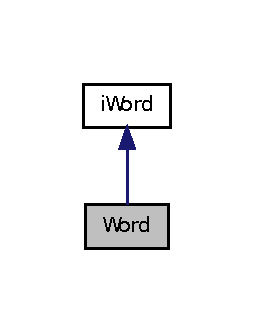
\includegraphics[width=122pt]{classWord__inherit__graph}
\end{center}
\end{figure}


Collaboration diagram for Word:\nopagebreak
\begin{figure}[H]
\begin{center}
\leavevmode
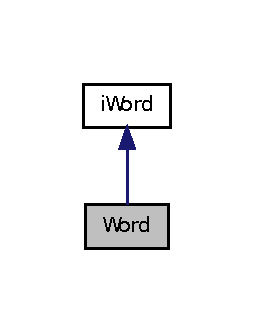
\includegraphics[width=122pt]{classWord__coll__graph}
\end{center}
\end{figure}
\subsection*{Public Member Functions}
\begin{DoxyCompactItemize}
\item 
int \hyperlink{classWord_a19303d963626549830a8da33d863bd6d}{toInt} () const 
\begin{DoxyCompactList}\small\item\em \char`\"{}To non-\/negative Integer\char`\"{} \item\end{DoxyCompactList}\item 
int \hyperlink{classWord_a3d771d68afd4a70d279af8bd9cd6bef9}{toInt2Complement} () const 
\begin{DoxyCompactList}\small\item\em \char`\"{}To Integer as 2's Complement\char`\"{} \item\end{DoxyCompactList}\item 
std::string \hyperlink{classWord_ac2ca49ef4da2fb57172fe057849e53fa}{toStr} () const 
\begin{DoxyCompactList}\small\item\em \char`\"{}To String\char`\"{} \item\end{DoxyCompactList}\item 
std::string \hyperlink{classWord_ab797467868642bb096bc4c9b1ed0a2f0}{toHex} () const 
\begin{DoxyCompactList}\small\item\em \char`\"{}To Hexadecimal\char`\"{} \item\end{DoxyCompactList}\item 
bool \hyperlink{classWord_ad6499f93b487d6d550a3fd4adcee9c8d}{fromInt} (int)
\begin{DoxyCompactList}\small\item\em \char`\"{}From Integer\char`\"{} \item\end{DoxyCompactList}\item 
bool \hyperlink{classWord_a614b52f3312d82ac5681403651040714}{fromStr} (const std::string \&)
\begin{DoxyCompactList}\small\item\em \char`\"{}From String\char`\"{} \item\end{DoxyCompactList}\item 
bool \hyperlink{classWord_a4e26eb82e8f7426dd46be2bbec9e41c5}{fromHex} (const std::string \&)
\begin{DoxyCompactList}\small\item\em \char`\"{}From Hexadecimal\char`\"{} \item\end{DoxyCompactList}\item 
\hyperlink{classWord}{Word} \hyperlink{classWord_a5cb9115a6cee6666e88390e56eb32071}{Add} (const \hyperlink{classiWord}{iWord} \&) const 
\begin{DoxyCompactList}\small\item\em Adds two words. \item\end{DoxyCompactList}\item 
\hyperlink{classWord}{Word} \hyperlink{classWord_a88e945efd81d13e15adb1ed9e4e95a5a}{operator+} (const \hyperlink{classiWord}{iWord} \&) const 
\begin{DoxyCompactList}\small\item\em A standard addition operator. \item\end{DoxyCompactList}\item 
\hyperlink{classWord}{Word} \hyperlink{classWord_a3ef457fb6f6ce54f5e98a83db4ae4472}{Subtract} (const \hyperlink{classiWord}{iWord} \&) const 
\begin{DoxyCompactList}\small\item\em Subtracts two words. \item\end{DoxyCompactList}\item 
\hyperlink{classWord}{Word} \hyperlink{classWord_a9ec270f103a3a755bd7b627e4b899bb4}{operator-\/} (const \hyperlink{classiWord}{iWord} \&) const 
\begin{DoxyCompactList}\small\item\em A standard subtraction operator. \item\end{DoxyCompactList}\item 
\hyperlink{classWord}{Word} \hyperlink{classWord_a4e1926ab5f4af7b63ec1bf4fadf873ad}{And} (const \hyperlink{classiWord}{iWord} \&) const 
\begin{DoxyCompactList}\small\item\em \char`\"{}And\char`\"{}s the bits of two words. \item\end{DoxyCompactList}\item 
\hypertarget{classWord_aa8645b9198fac6d0833b32503db6e18a}{
\hyperlink{classWord}{Word} {\bfseries Or} (const \hyperlink{classiWord}{iWord} \&) const }
\label{classWord_aa8645b9198fac6d0833b32503db6e18a}

\item 
\hypertarget{classWord_afdecfa9e3f2fda36496f249617a4cef5}{
\hyperlink{classWord}{Word} {\bfseries Not} () const }
\label{classWord_afdecfa9e3f2fda36496f249617a4cef5}

\item 
void \hyperlink{classWord_abb97142e332c7cc25d2a0c2bdb6c3d9b}{copy} (const \hyperlink{classiWord}{iWord} \&)
\begin{DoxyCompactList}\small\item\em Copies a word. \item\end{DoxyCompactList}\item 
\hyperlink{classWord}{Word} \& \hyperlink{classWord_a2ae41869cb0f1855fc18c6bce05f7c4d}{operator=} (const \hyperlink{classWord}{Word})
\begin{DoxyCompactList}\small\item\em A standard assignment operator. \item\end{DoxyCompactList}\item 
\hyperlink{classiWord}{iWord} \& \hyperlink{classWord_a3837f49bcb44597e6d738ccb0eeed144}{operator++} ()
\item 
\hyperlink{classiWord}{iWord} \& \hyperlink{classWord_ae921b75d263be790fd150c5962445163}{operator++} (int)
\begin{DoxyCompactList}\small\item\em A standard post-\/increment operator. \item\end{DoxyCompactList}\item 
bool \hyperlink{classWord_ab0f10ac1a0397559b859774b503538fe}{operator\mbox{[}$\,$\mbox{]}} (const int) const 
\begin{DoxyCompactList}\small\item\em An accessor to the \char`\"{}i\char`\"{}th bit of the value. \item\end{DoxyCompactList}\item 
\hypertarget{classWord_a7484e0f4d1fa712ca367539dad71dfa3}{
void {\bfseries print} () const }
\label{classWord_a7484e0f4d1fa712ca367539dad71dfa3}

\end{DoxyCompactItemize}
\subsection*{Private Member Functions}
\begin{DoxyCompactItemize}
\item 
\hypertarget{classWord_aaacae836ba9ed28f9725432ae81ab318}{
bool {\bfseries \_\-hasBit} (int) const }
\label{classWord_aaacae836ba9ed28f9725432ae81ab318}

\end{DoxyCompactItemize}
\subsection*{Private Attributes}
\begin{DoxyCompactItemize}
\item 
\hypertarget{classWord_a8b0aa1f2042266f307c51b3bdafa9128}{
unsigned short {\bfseries \_\-value}}
\label{classWord_a8b0aa1f2042266f307c51b3bdafa9128}

\end{DoxyCompactItemize}


\subsection{Member Function Documentation}
\hypertarget{classWord_a19303d963626549830a8da33d863bd6d}{
\index{Word@{Word}!toInt@{toInt}}
\index{toInt@{toInt}!Word@{Word}}
\subsubsection[{toInt}]{\setlength{\rightskip}{0pt plus 5cm}int Word::toInt (
\begin{DoxyParamCaption}
{}
\end{DoxyParamCaption}
) const\hspace{0.3cm}{\ttfamily  \mbox{[}virtual\mbox{]}}}}
\label{classWord_a19303d963626549830a8da33d863bd6d}


\char`\"{}To non-\/negative Integer\char`\"{} 

\begin{DoxyPostcond}{Postcondition}
The value of the word is not changed. 
\end{DoxyPostcond}
\begin{DoxyReturn}{Returns}
The bits of the word interpreted as a positive integer value. 
\end{DoxyReturn}


Implements \hyperlink{classiWord_a3349d0a243d3432bb35b76af8420b1d9}{iWord}.

\hypertarget{classWord_a3d771d68afd4a70d279af8bd9cd6bef9}{
\index{Word@{Word}!toInt2Complement@{toInt2Complement}}
\index{toInt2Complement@{toInt2Complement}!Word@{Word}}
\subsubsection[{toInt2Complement}]{\setlength{\rightskip}{0pt plus 5cm}int Word::toInt2Complement (
\begin{DoxyParamCaption}
{}
\end{DoxyParamCaption}
) const\hspace{0.3cm}{\ttfamily  \mbox{[}virtual\mbox{]}}}}
\label{classWord_a3d771d68afd4a70d279af8bd9cd6bef9}


\char`\"{}To Integer as 2's Complement\char`\"{} 

\begin{DoxyPostcond}{Postcondition}
The value of the word is not changed. 
\end{DoxyPostcond}
\begin{DoxyReturn}{Returns}
The bits of the word interpreted as a signed (2's complement) integer value. 
\end{DoxyReturn}


Implements \hyperlink{classiWord_a1377d01257b792c748b013be60b089e6}{iWord}.

\hypertarget{classWord_ac2ca49ef4da2fb57172fe057849e53fa}{
\index{Word@{Word}!toStr@{toStr}}
\index{toStr@{toStr}!Word@{Word}}
\subsubsection[{toStr}]{\setlength{\rightskip}{0pt plus 5cm}string Word::toStr (
\begin{DoxyParamCaption}
{}
\end{DoxyParamCaption}
) const\hspace{0.3cm}{\ttfamily  \mbox{[}virtual\mbox{]}}}}
\label{classWord_ac2ca49ef4da2fb57172fe057849e53fa}


\char`\"{}To String\char`\"{} 

\begin{DoxyPostcond}{Postcondition}
The value of the word is not changed. 
\end{DoxyPostcond}
\begin{DoxyReturn}{Returns}
\char`\"{}\mbox{[}\char`\"{} + $<$16 characters: either 1's or 0's$>$ + \char`\"{}\mbox{]}\char`\"{}
\end{DoxyReturn}
\begin{DoxyParagraph}{Examples:}
If the object holds a (2's comp.) value 4: \mbox{[}0000000000000100\mbox{]}\par
 If the object holds a (2's comp.) value -\/1: \mbox{[}1111111111111111\mbox{]} 
\end{DoxyParagraph}


Implements \hyperlink{classiWord_a0114861c4b660286834ad637f11dc4f4}{iWord}.

\hypertarget{classWord_ab797467868642bb096bc4c9b1ed0a2f0}{
\index{Word@{Word}!toHex@{toHex}}
\index{toHex@{toHex}!Word@{Word}}
\subsubsection[{toHex}]{\setlength{\rightskip}{0pt plus 5cm}string Word::toHex (
\begin{DoxyParamCaption}
{}
\end{DoxyParamCaption}
) const\hspace{0.3cm}{\ttfamily  \mbox{[}virtual\mbox{]}}}}
\label{classWord_ab797467868642bb096bc4c9b1ed0a2f0}


\char`\"{}To Hexadecimal\char`\"{} 

\begin{DoxyPostcond}{Postcondition}
The value of the word is not changed. 
\end{DoxyPostcond}
\begin{DoxyReturn}{Returns}
\char`\"{}0x\char`\"{} + $<$4 characters in the range \mbox{[}0-\/9\mbox{]},\mbox{[}A-\/F\mbox{]}$>$
\end{DoxyReturn}
\begin{DoxyParagraph}{Examples:}
If the object holds (2's comp.) value 8: 0x0008\par
 If the object holds (2's comp.) value -\/2: 0xFFFE 
\end{DoxyParagraph}


Implements \hyperlink{classiWord_a7fc28d0251f8acb4dc3f388fc25c57d1}{iWord}.

\hypertarget{classWord_ad6499f93b487d6d550a3fd4adcee9c8d}{
\index{Word@{Word}!fromInt@{fromInt}}
\index{fromInt@{fromInt}!Word@{Word}}
\subsubsection[{fromInt}]{\setlength{\rightskip}{0pt plus 5cm}bool Word::fromInt (
\begin{DoxyParamCaption}
\item[{int}]{}
\end{DoxyParamCaption}
)\hspace{0.3cm}{\ttfamily  \mbox{[}virtual\mbox{]}}}}
\label{classWord_ad6499f93b487d6d550a3fd4adcee9c8d}


\char`\"{}From Integer\char`\"{} 


\begin{DoxyParams}[1]{Parameters}
\mbox{\tt in}  & {\em value} & The value to be stored into the word. \\
\hline
\end{DoxyParams}
\begin{DoxyPostcond}{Postcondition}
\char`\"{}value\char`\"{} is not changed. 
\end{DoxyPostcond}
\begin{DoxyReturn}{Returns}
True if and only if \char`\"{}value\char`\"{} can be represented in 16 bits
\end{DoxyReturn}
When this function returns \char`\"{}False\char`\"{}, the value of the word is unchanged.\par
 Otherwise, the word now holds the value \char`\"{}value\char`\"{}. 

Implements \hyperlink{classiWord_a6421bf139c6eb4044446997606cb65e7}{iWord}.

\hypertarget{classWord_a614b52f3312d82ac5681403651040714}{
\index{Word@{Word}!fromStr@{fromStr}}
\index{fromStr@{fromStr}!Word@{Word}}
\subsubsection[{fromStr}]{\setlength{\rightskip}{0pt plus 5cm}bool Word::fromStr (
\begin{DoxyParamCaption}
\item[{const std::string \&}]{}
\end{DoxyParamCaption}
)\hspace{0.3cm}{\ttfamily  \mbox{[}virtual\mbox{]}}}}
\label{classWord_a614b52f3312d82ac5681403651040714}


\char`\"{}From String\char`\"{} 


\begin{DoxyParams}[1]{Parameters}
\mbox{\tt in}  & {\em str} & A string of characters meant to represent a \char`\"{}word\char`\"{} to be stored. \\
\hline
\end{DoxyParams}
\begin{DoxyPostcond}{Postcondition}
\char`\"{}str\char`\"{} is not changed. 
\end{DoxyPostcond}
\begin{DoxyReturn}{Returns}
True if and only if \char`\"{}str\char`\"{} is well-\/formed (as defined in \hyperlink{classWord_ac2ca49ef4da2fb57172fe057849e53fa}{toStr()}).
\end{DoxyReturn}
When this function returns \char`\"{}False\char`\"{}, the value of the word is unchanged.\par
 Otherwise, the word now holds the value \char`\"{}str\char`\"{}. 

Implements \hyperlink{classiWord_ad8df9e06ccb87d1e65766120713ef545}{iWord}.

\hypertarget{classWord_a4e26eb82e8f7426dd46be2bbec9e41c5}{
\index{Word@{Word}!fromHex@{fromHex}}
\index{fromHex@{fromHex}!Word@{Word}}
\subsubsection[{fromHex}]{\setlength{\rightskip}{0pt plus 5cm}bool Word::fromHex (
\begin{DoxyParamCaption}
\item[{const std::string \&}]{}
\end{DoxyParamCaption}
)\hspace{0.3cm}{\ttfamily  \mbox{[}virtual\mbox{]}}}}
\label{classWord_a4e26eb82e8f7426dd46be2bbec9e41c5}


\char`\"{}From Hexadecimal\char`\"{} 


\begin{DoxyParams}[1]{Parameters}
\mbox{\tt in}  & {\em str} & A string of characters meant to represent a \char`\"{}word\char`\"{} to be stored. \\
\hline
\end{DoxyParams}
\begin{DoxyPostcond}{Postcondition}
\char`\"{}str\char`\"{} is not changed. 
\end{DoxyPostcond}
\begin{DoxyReturn}{Returns}
True if and only if \char`\"{}str\char`\"{} is well-\/formed (as defined in \hyperlink{classWord_ab797467868642bb096bc4c9b1ed0a2f0}{toHex()}).
\end{DoxyReturn}
When this function returns \char`\"{}False\char`\"{}, the value of the word is unchanged.\par
 Otherwise, the word now holds the value \char`\"{}str\char`\"{}. 

Implements \hyperlink{classiWord_a0c08832b3e9b41073fc6666407ef8c53}{iWord}.

\hypertarget{classWord_a5cb9115a6cee6666e88390e56eb32071}{
\index{Word@{Word}!Add@{Add}}
\index{Add@{Add}!Word@{Word}}
\subsubsection[{Add}]{\setlength{\rightskip}{0pt plus 5cm}{\bf Word} Word::Add (
\begin{DoxyParamCaption}
\item[{const {\bf iWord} \&}]{}
\end{DoxyParamCaption}
) const\hspace{0.3cm}{\ttfamily  \mbox{[}virtual\mbox{]}}}}
\label{classWord_a5cb9115a6cee6666e88390e56eb32071}


Adds two words. 


\begin{DoxyParams}[1]{Parameters}
\mbox{\tt in}  & {\em w} & A word value to be added. \\
\hline
\end{DoxyParams}
\begin{DoxyPostcond}{Postcondition}
Both \char`\"{}w\char`\"{} and the calling object do not change. 
\end{DoxyPostcond}
\begin{DoxyReturn}{Returns}
A new \char`\"{}Word\char`\"{} object containing result of adding \char`\"{}w\char`\"{} and the calling object.
\end{DoxyReturn}
\begin{DoxyNote}{Note}
The addition is carried out with no regard to logical overflow. 
\end{DoxyNote}


Implements \hyperlink{classiWord_a999c52ac2e7abf756eeb16fe5b31aad7}{iWord}.

\hypertarget{classWord_a88e945efd81d13e15adb1ed9e4e95a5a}{
\index{Word@{Word}!operator+@{operator+}}
\index{operator+@{operator+}!Word@{Word}}
\subsubsection[{operator+}]{\setlength{\rightskip}{0pt plus 5cm}{\bf Word} Word::operator+ (
\begin{DoxyParamCaption}
\item[{const {\bf iWord} \&}]{}
\end{DoxyParamCaption}
) const\hspace{0.3cm}{\ttfamily  \mbox{[}virtual\mbox{]}}}}
\label{classWord_a88e945efd81d13e15adb1ed9e4e95a5a}


A standard addition operator. 

\begin{DoxyNote}{Note}
\char`\"{}result = p + w\char`\"{} is equivalent to \char`\"{}result = p.Add(w)\char`\"{}. 
\end{DoxyNote}


Implements \hyperlink{classiWord_a8dfb66b7cd91fe0a4169f071c1f9bc53}{iWord}.

\hypertarget{classWord_a3ef457fb6f6ce54f5e98a83db4ae4472}{
\index{Word@{Word}!Subtract@{Subtract}}
\index{Subtract@{Subtract}!Word@{Word}}
\subsubsection[{Subtract}]{\setlength{\rightskip}{0pt plus 5cm}{\bf Word} Word::Subtract (
\begin{DoxyParamCaption}
\item[{const {\bf iWord} \&}]{}
\end{DoxyParamCaption}
) const\hspace{0.3cm}{\ttfamily  \mbox{[}virtual\mbox{]}}}}
\label{classWord_a3ef457fb6f6ce54f5e98a83db4ae4472}


Subtracts two words. 


\begin{DoxyParams}[1]{Parameters}
\mbox{\tt in}  & {\em w} & A word value to be subtracted. \\
\hline
\end{DoxyParams}
\begin{DoxyPostcond}{Postcondition}
Both \char`\"{}w\char`\"{} and the calling object do not change. 
\end{DoxyPostcond}
\begin{DoxyReturn}{Returns}
A new \char`\"{}Word\char`\"{} object containing the result of subtracting \char`\"{}w\char`\"{} from the calling object.
\end{DoxyReturn}
\begin{DoxyNote}{Note}
The subtraction is carried out with no regard for logical overflow. 
\end{DoxyNote}


Implements \hyperlink{classiWord_af69a5e10e094e3fc30fae0b651d95ea6}{iWord}.

\hypertarget{classWord_a9ec270f103a3a755bd7b627e4b899bb4}{
\index{Word@{Word}!operator-\/@{operator-\/}}
\index{operator-\/@{operator-\/}!Word@{Word}}
\subsubsection[{operator-\/}]{\setlength{\rightskip}{0pt plus 5cm}{\bf Word} Word::operator-\/ (
\begin{DoxyParamCaption}
\item[{const {\bf iWord} \&}]{}
\end{DoxyParamCaption}
) const\hspace{0.3cm}{\ttfamily  \mbox{[}virtual\mbox{]}}}}
\label{classWord_a9ec270f103a3a755bd7b627e4b899bb4}


A standard subtraction operator. 

\begin{DoxyNote}{Note}
\char`\"{}result = p -\/ w\char`\"{} is equivalent to \char`\"{}result = p.Subtract(w)\char`\"{}. 
\end{DoxyNote}


Implements \hyperlink{classiWord_a432fb05081debadb601d86cca05152c8}{iWord}.

\hypertarget{classWord_a4e1926ab5f4af7b63ec1bf4fadf873ad}{
\index{Word@{Word}!And@{And}}
\index{And@{And}!Word@{Word}}
\subsubsection[{And}]{\setlength{\rightskip}{0pt plus 5cm}{\bf Word} Word::And (
\begin{DoxyParamCaption}
\item[{const {\bf iWord} \&}]{}
\end{DoxyParamCaption}
) const\hspace{0.3cm}{\ttfamily  \mbox{[}virtual\mbox{]}}}}
\label{classWord_a4e1926ab5f4af7b63ec1bf4fadf873ad}


\char`\"{}And\char`\"{}s the bits of two words. 


\begin{DoxyParams}[1]{Parameters}
\mbox{\tt in}  & {\em w} & A word value to be \char`\"{}and\char`\"{}ed. \\
\hline
\end{DoxyParams}
\begin{DoxyPostcond}{Postcondition}
Both \char`\"{}w\char`\"{} and the calling object do not change. 
\end{DoxyPostcond}
\begin{DoxyReturn}{Returns}
A new \char`\"{}Word\char`\"{} object containing the result of performing a bit-\/wise and on \char`\"{}w\char`\"{} and the calling object. 
\end{DoxyReturn}


Implements \hyperlink{classiWord_ae9f6bbc855712a208835d12cb3e40577}{iWord}.

\hypertarget{classWord_abb97142e332c7cc25d2a0c2bdb6c3d9b}{
\index{Word@{Word}!copy@{copy}}
\index{copy@{copy}!Word@{Word}}
\subsubsection[{copy}]{\setlength{\rightskip}{0pt plus 5cm}void Word::copy (
\begin{DoxyParamCaption}
\item[{const {\bf iWord} \&}]{}
\end{DoxyParamCaption}
)\hspace{0.3cm}{\ttfamily  \mbox{[}virtual\mbox{]}}}}
\label{classWord_abb97142e332c7cc25d2a0c2bdb6c3d9b}


Copies a word. 


\begin{DoxyParams}[1]{Parameters}
\mbox{\tt out}  & {\em The} & value to be copied. \\
\hline
\end{DoxyParams}
\begin{DoxyPostcond}{Postcondition}
The caller equals that parameter.
\end{DoxyPostcond}
Equivalent to the assignment \char`\"{}caller = parameter\char`\"{}. 

Implements \hyperlink{classiWord_ab9f5df8ced4937c18f16784a98ecf95f}{iWord}.

\hypertarget{classWord_a2ae41869cb0f1855fc18c6bce05f7c4d}{
\index{Word@{Word}!operator=@{operator=}}
\index{operator=@{operator=}!Word@{Word}}
\subsubsection[{operator=}]{\setlength{\rightskip}{0pt plus 5cm}{\bf Word} \& Word::operator= (
\begin{DoxyParamCaption}
\item[{const }]{ Word}
\end{DoxyParamCaption}
)\hspace{0.3cm}{\ttfamily  \mbox{[}virtual\mbox{]}}}}
\label{classWord_a2ae41869cb0f1855fc18c6bce05f7c4d}


A standard assignment operator. 


\begin{DoxyParams}[1]{Parameters}
\mbox{\tt in}  & {\em The} & value to be copied. \\
\hline
\end{DoxyParams}
\begin{DoxyReturn}{Returns}
A copy of the parameter.
\end{DoxyReturn}
The return value and parameter here must be declared as \char`\"{}Word\char`\"{}s as C++ does not work well with polymorphic assignment operators. 

Implements \hyperlink{classiWord_a45c9c82054bd2150b77d5f157734cb72}{iWord}.

\hypertarget{classWord_a3837f49bcb44597e6d738ccb0eeed144}{
\index{Word@{Word}!operator++@{operator++}}
\index{operator++@{operator++}!Word@{Word}}
\subsubsection[{operator++}]{\setlength{\rightskip}{0pt plus 5cm}{\bf iWord} \& Word::operator++ (
\begin{DoxyParamCaption}
{}
\end{DoxyParamCaption}
)\hspace{0.3cm}{\ttfamily  \mbox{[}virtual\mbox{]}}}}
\label{classWord_a3837f49bcb44597e6d738ccb0eeed144}
A standard pre-\/increment operator. \begin{DoxyReturn}{Returns}
A reference to itself.
\end{DoxyReturn}
The object increments its value BEFORE the execution of the current line. 

Implements \hyperlink{classiWord_af20040c25b79d2aeae41f1714fbb2cbc}{iWord}.

\hypertarget{classWord_ae921b75d263be790fd150c5962445163}{
\index{Word@{Word}!operator++@{operator++}}
\index{operator++@{operator++}!Word@{Word}}
\subsubsection[{operator++}]{\setlength{\rightskip}{0pt plus 5cm}{\bf iWord} \& Word::operator++ (
\begin{DoxyParamCaption}
\item[{int}]{}
\end{DoxyParamCaption}
)\hspace{0.3cm}{\ttfamily  \mbox{[}virtual\mbox{]}}}}
\label{classWord_ae921b75d263be790fd150c5962445163}


A standard post-\/increment operator. 

\begin{DoxyReturn}{Returns}
A reference to itself.
\end{DoxyReturn}
The object increments its value AFTER the execution of the current line. 

Implements \hyperlink{classiWord_a6777f6f41915179c4255d3647a9eb4b5}{iWord}.

\hypertarget{classWord_ab0f10ac1a0397559b859774b503538fe}{
\index{Word@{Word}!operator\mbox{[}\mbox{]}@{operator[]}}
\index{operator\mbox{[}\mbox{]}@{operator[]}!Word@{Word}}
\subsubsection[{operator[]}]{\setlength{\rightskip}{0pt plus 5cm}bool Word::operator\mbox{[}$\,$\mbox{]} (
\begin{DoxyParamCaption}
\item[{const }]{}
\end{DoxyParamCaption}
) const\hspace{0.3cm}{\ttfamily  \mbox{[}virtual\mbox{]}}}}
\label{classWord_ab0f10ac1a0397559b859774b503538fe}


An accessor to the \char`\"{}i\char`\"{}th bit of the value. 


\begin{DoxyParams}[1]{Parameters}
\mbox{\tt in}  & {\em The} & index of the bit in question. \\
\hline
\end{DoxyParams}
\begin{DoxyPrecond}{Precondition}
The index must be less than the size of a word, ie. 16. 
\end{DoxyPrecond}
\begin{DoxyReturn}{Returns}
True $<$=$>$ 1, False $<$=$>$ 0.
\end{DoxyReturn}
The number of the bits starts at zero and rises into the more significant bits. Examples: If the object \char`\"{}num\char`\"{} holds a value of 4 (0...100 in binary), num\mbox{[}0\mbox{]} = 0, num\mbox{[}1\mbox{]} = 0, num\mbox{[}2\mbox{]} = 1. If it holds a value of 1 (0...001 in binary) num\mbox{[}0\mbox{]} = 1, num\mbox{[}1\mbox{]} = 0, num\mbox{[}2\mbox{]} = 0, etc. If it holds a negative value (Starting with a 1 in 2's complement), num\mbox{[}15\mbox{]} = 1. 

Implements \hyperlink{classiWord_a2bd140904379329b74c3e1af83eb3a85}{iWord}.



The documentation for this class was generated from the following files:\begin{DoxyCompactItemize}
\item 
Word.h\item 
Word.cpp\end{DoxyCompactItemize}

\chapter{File Documentation}
\hypertarget{Decoder_8h}{
\section{Decoder.h File Reference}
\label{Decoder_8h}\index{Decoder.h@{Decoder.h}}
}


Definition of the private data for the \char`\"{}Decoder\char`\"{} class. (none)  


Include dependency graph for Decoder.h:\nopagebreak
\begin{figure}[H]
\begin{center}
\leavevmode
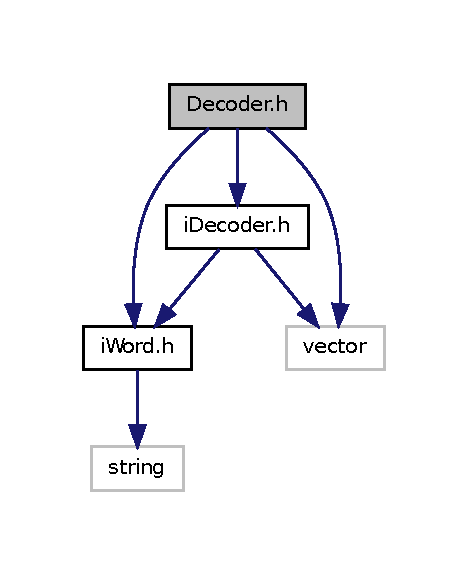
\includegraphics[width=224pt]{Decoder_8h__incl}
\end{center}
\end{figure}
\subsection*{Classes}
\begin{DoxyCompactItemize}
\item 
class \hyperlink{classDecoder}{Decoder}
\begin{DoxyCompactList}\small\item\em Implements \hyperlink{classiDecoder}{iDecoder}. \item\end{DoxyCompactList}\end{DoxyCompactItemize}


\subsection{Detailed Description}
Definition of the private data for the \char`\"{}Decoder\char`\"{} class. (none) \begin{DoxyAuthor}{Author}
Andrew Canale 

Andrew Groot 
\end{DoxyAuthor}

\hypertarget{iDecoder_8h}{
\section{iDecoder.h File Reference}
\label{iDecoder_8h}\index{iDecoder.h@{iDecoder.h}}
}


Definition of the Wi-\/11 instruction decoder.  


Include dependency graph for iDecoder.h:\nopagebreak
\begin{figure}[H]
\begin{center}
\leavevmode
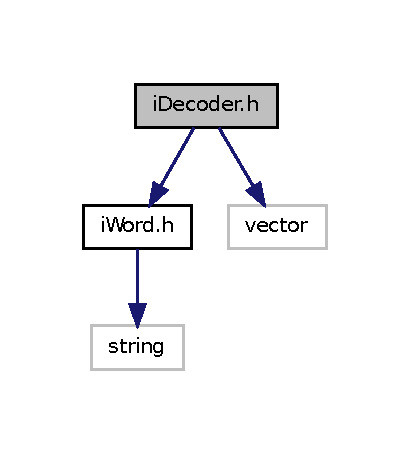
\includegraphics[width=196pt]{iDecoder_8h__incl}
\end{center}
\end{figure}
\subsection*{Classes}
\begin{DoxyCompactItemize}
\item 
class \hyperlink{classiDecoder}{iDecoder}
\begin{DoxyCompactList}\small\item\em Defines how Wi-\/11 instructions are decoded. \item\end{DoxyCompactList}\item 
struct \hyperlink{structInstruction}{Instruction}
\begin{DoxyCompactList}\small\item\em Container to simplify interactions with Wi-\/11 instructions. \item\end{DoxyCompactList}\end{DoxyCompactItemize}
\subsection*{Namespaces}
\begin{DoxyCompactItemize}
\item 
namespace \hyperlink{namespaceDecoder__Directory}{Decoder\_\-Directory}


\begin{DoxyCompactList}\small\item\em Declares register id's and instruction types for each register and instruction. \item\end{DoxyCompactList}

\end{DoxyCompactItemize}
\subsection*{Enumerations}
\begin{DoxyCompactItemize}
\item 
enum {\bfseries INSTRUCTION\_\-TYPE} \{ \par
{\bfseries ADD}, 
{\bfseries AND}, 
{\bfseries BRx}, 
{\bfseries DBUG}, 
\par
{\bfseries JSR}, 
{\bfseries JSRR}, 
{\bfseries LD}, 
{\bfseries LDI}, 
\par
{\bfseries LDR}, 
{\bfseries LEA}, 
{\bfseries NOT}, 
{\bfseries RET}, 
\par
{\bfseries ST}, 
{\bfseries STI}, 
{\bfseries STR}, 
{\bfseries TRAP}, 
\par
{\bfseries ERROR}
 \}
\item 
enum {\bfseries REGISTER\_\-ID} \{ \par
{\bfseries R0}, 
{\bfseries R1}, 
{\bfseries R2}, 
{\bfseries R3}, 
\par
{\bfseries R4}, 
{\bfseries R5}, 
{\bfseries R6}, 
{\bfseries R7}, 
\par
{\bfseries PC}
 \}
\end{DoxyCompactItemize}


\subsection{Detailed Description}
Definition of the Wi-\/11 instruction decoder. \begin{DoxyAuthor}{Author}
Joshua Green 

Andrew Groot 
\end{DoxyAuthor}

\hypertarget{iLoader_8h}{
\section{iLoader.h File Reference}
\label{iLoader_8h}\index{iLoader.h@{iLoader.h}}
}


Definition of the Wi-\/11 program loader.  


Include dependency graph for iLoader.h:\nopagebreak
\begin{figure}[H]
\begin{center}
\leavevmode
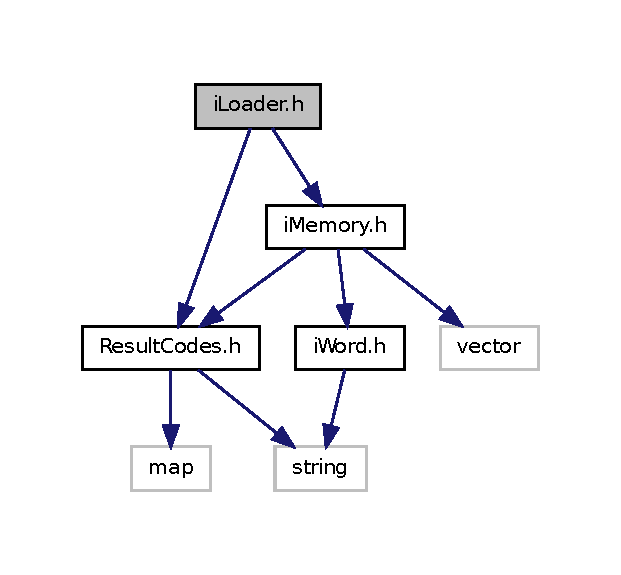
\includegraphics[width=298pt]{iLoader_8h__incl}
\end{center}
\end{figure}
\subsection*{Classes}
\begin{DoxyCompactItemize}
\item 
class \hyperlink{classiLoader}{iLoader}
\begin{DoxyCompactList}\small\item\em Defines how the Wi-\/11 initializes memory. \item\end{DoxyCompactList}\end{DoxyCompactItemize}


\subsection{Detailed Description}
Definition of the Wi-\/11 program loader. \begin{DoxyAuthor}{Author}
Joshua Green 

Andrew Groot 
\end{DoxyAuthor}

\hypertarget{iMemory_8h}{
\section{iMemory.h File Reference}
\label{iMemory_8h}\index{iMemory.h@{iMemory.h}}
}


Definition of Wi-\/11 memory.  


Include dependency graph for iMemory.h:\nopagebreak
\begin{figure}[H]
\begin{center}
\leavevmode
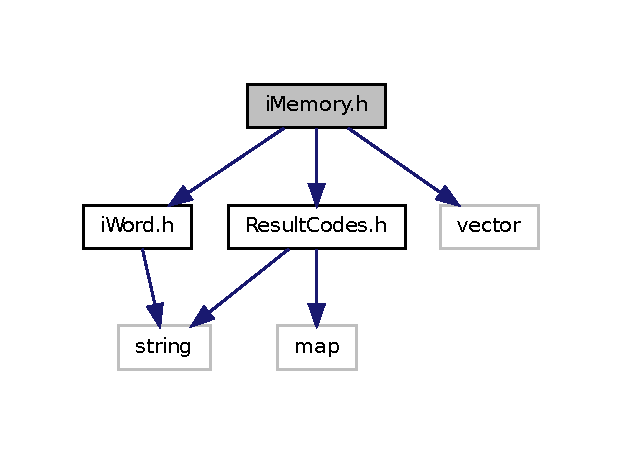
\includegraphics[width=298pt]{iMemory_8h__incl}
\end{center}
\end{figure}
\subsection*{Classes}
\begin{DoxyCompactItemize}
\item 
class \hyperlink{classiMemory}{iMemory}
\begin{DoxyCompactList}\small\item\em Defines the functionality of memory in the Wi-\/11 machine. \item\end{DoxyCompactList}\end{DoxyCompactItemize}


\subsection{Detailed Description}
Definition of Wi-\/11 memory. \begin{DoxyAuthor}{Author}
Joshua Green 

Andrew Groot 
\end{DoxyAuthor}

\hypertarget{iObjParser_8h}{
\section{iObjParser.h File Reference}
\label{iObjParser_8h}\index{iObjParser.h@{iObjParser.h}}
}
Include dependency graph for iObjParser.h:
\nopagebreak
\begin{figure}[H]
\begin{center}
\leavevmode
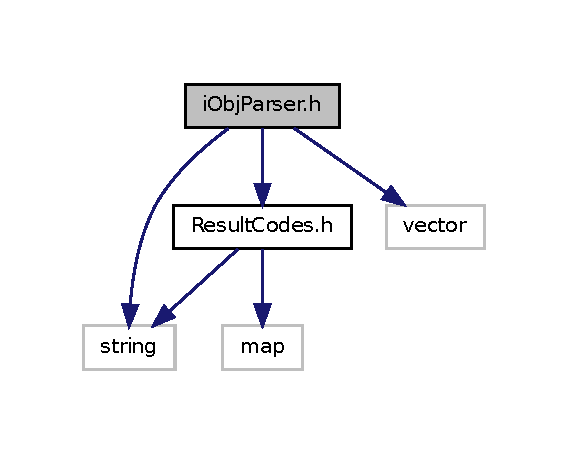
\includegraphics[width=272pt]{iObjParser_8h__incl}
\end{center}
\end{figure}
\subsection*{Classes}
\begin{DoxyCompactItemize}
\item 
struct \hyperlink{structObjectData}{ObjectData}
\begin{DoxyCompactList}\small\item\em A simple encoding of a \char`\"{}record\char`\"{}. \item\end{DoxyCompactList}\item 
class \hyperlink{classiObjParser}{iObjParser}
\begin{DoxyCompactList}\small\item\em Defines how object files are processed. \item\end{DoxyCompactList}\end{DoxyCompactItemize}


\subsection{Detailed Description}
\begin{DoxyAuthor}{Author}
Joshua Green 

Andrew Groot  of the Object File Parser. 
\end{DoxyAuthor}

\hypertarget{iRegister_8h}{
\section{iRegister.h File Reference}
\label{iRegister_8h}\index{iRegister.h@{iRegister.h}}
}


Definition of a \char`\"{}register\char`\"{} in the Wi-\/11 machine.  


Include dependency graph for iRegister.h:
\nopagebreak
\begin{figure}[H]
\begin{center}
\leavevmode
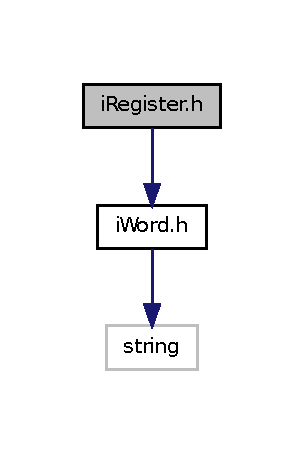
\includegraphics[width=144pt]{iRegister_8h__incl}
\end{center}
\end{figure}
This graph shows which files directly or indirectly include this file:
\nopagebreak
\begin{figure}[H]
\begin{center}
\leavevmode
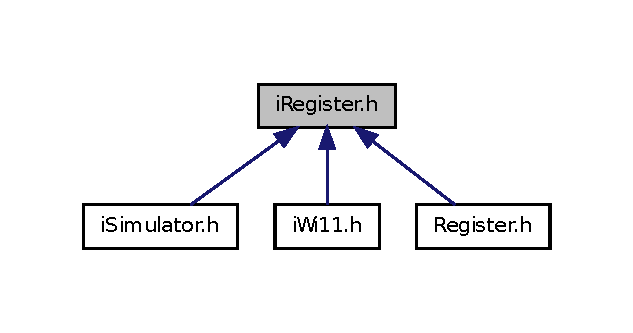
\includegraphics[width=302pt]{iRegister_8h__dep__incl}
\end{center}
\end{figure}
\subsection*{Classes}
\begin{DoxyCompactItemize}
\item 
class \hyperlink{classiRegister}{iRegister}
\begin{DoxyCompactList}\small\item\em Defines a \char`\"{}register\char`\"{} in the Wi-\/11 machine. \item\end{DoxyCompactList}\end{DoxyCompactItemize}


\subsection{Detailed Description}
Definition of a \char`\"{}register\char`\"{} in the Wi-\/11 machine. \begin{DoxyAuthor}{Author}
Joshua Green 

Andrew Groot 
\end{DoxyAuthor}

\hypertarget{iWi11_8h}{
\section{iWi11.h File Reference}
\label{iWi11_8h}\index{iWi11.h@{iWi11.h}}
}


Definition of the Wi-\/11 machine simulator.  


Include dependency graph for iWi11.h:\nopagebreak
\begin{figure}[H]
\begin{center}
\leavevmode
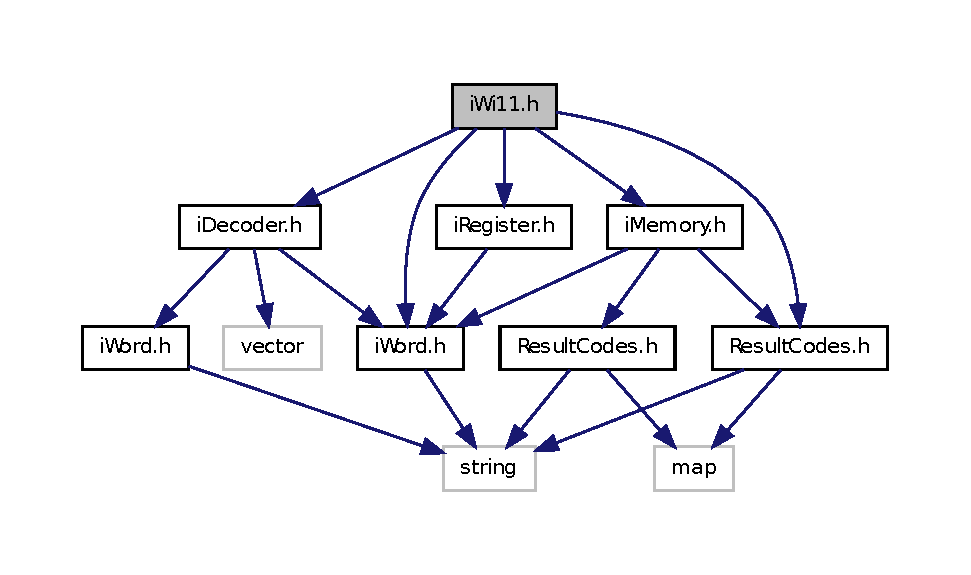
\includegraphics[width=400pt]{iWi11_8h__incl}
\end{center}
\end{figure}
\subsection*{Classes}
\begin{DoxyCompactItemize}
\item 
class \hyperlink{classiWi11}{iWi11}
\begin{DoxyCompactList}\small\item\em Defines the internal logic of the Wi-\/11. \item\end{DoxyCompactList}\end{DoxyCompactItemize}


\subsection{Detailed Description}
Definition of the Wi-\/11 machine simulator. \begin{DoxyAuthor}{Author}
Joshua Green 

Andrew Groot 
\end{DoxyAuthor}

\hypertarget{iWord_8h}{
\section{iWord.h File Reference}
\label{iWord_8h}\index{iWord.h@{iWord.h}}
}


The interface implemented by the \char`\"{}Word\char`\"{} class.  


Include dependency graph for iWord.h:\nopagebreak
\begin{figure}[H]
\begin{center}
\leavevmode
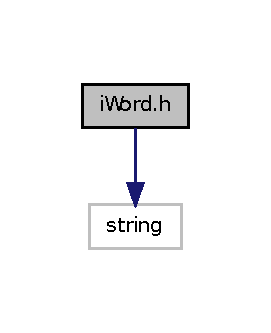
\includegraphics[width=130pt]{iWord_8h__incl}
\end{center}
\end{figure}
This graph shows which files directly or indirectly include this file:\nopagebreak
\begin{figure}[H]
\begin{center}
\leavevmode
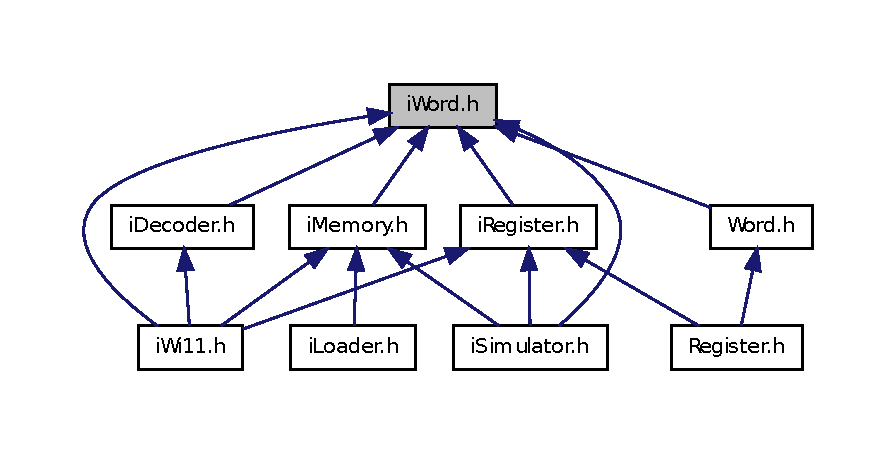
\includegraphics[width=400pt]{iWord_8h__dep__incl}
\end{center}
\end{figure}
\subsection*{Data Structures}
\begin{DoxyCompactItemize}
\item 
class \hyperlink{classiWord}{iWord}
\begin{DoxyCompactList}\small\item\em The \hyperlink{classiWord}{iWord} interface class defines the a \char`\"{}word\char`\"{} of data on the Wi-\/11 Machine. \item\end{DoxyCompactList}\end{DoxyCompactItemize}


\subsection{Detailed Description}
The interface implemented by the \char`\"{}Word\char`\"{} class. \begin{DoxyAuthor}{Author}
Joshua Green 

Andrew Groot
\end{DoxyAuthor}
Defines the operations and signatures by which the \char`\"{}Word\char`\"{} class should operate. The signatures, while intended to be coded to the interface, are done as to this as C++ allows. 
\hypertarget{Loader_8h}{
\section{Loader.h File Reference}
\label{Loader_8h}\index{Loader.h@{Loader.h}}
}


Definition of the private data for the \char`\"{}Loader\char`\"{} class.  


Include dependency graph for Loader.h:\nopagebreak
\begin{figure}[H]
\begin{center}
\leavevmode
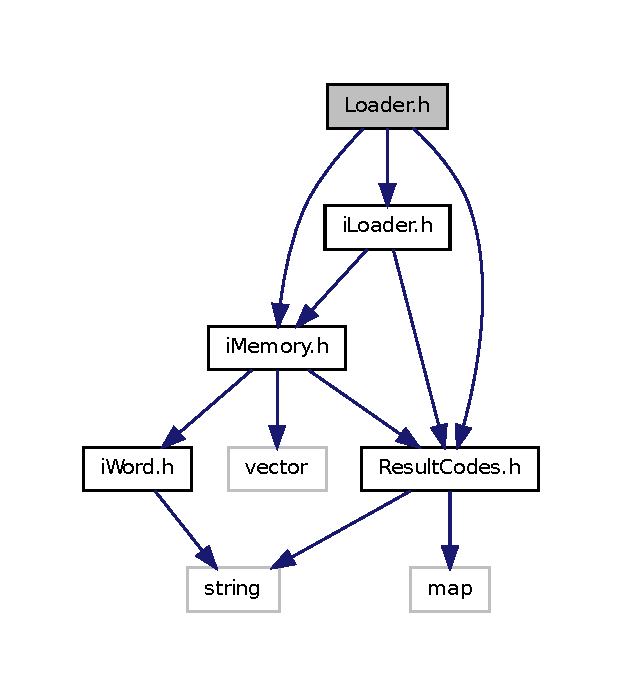
\includegraphics[width=298pt]{Loader_8h__incl}
\end{center}
\end{figure}
\subsection*{Classes}
\begin{DoxyCompactItemize}
\item 
class \hyperlink{classLoader}{Loader}
\begin{DoxyCompactList}\small\item\em Implements \hyperlink{classiLoader}{iLoader}. \item\end{DoxyCompactList}\end{DoxyCompactItemize}


\subsection{Detailed Description}
Definition of the private data for the \char`\"{}Loader\char`\"{} class. \begin{DoxyAuthor}{Author}
Logan Coulson 

Joshua Green 

Andrew Groot 
\end{DoxyAuthor}

\hypertarget{Memory_8h}{
\section{Memory.h File Reference}
\label{Memory_8h}\index{Memory.h@{Memory.h}}
}


Definition of private data for the \char`\"{}Memory\char`\"{} class.  


Include dependency graph for Memory.h:\nopagebreak
\begin{figure}[H]
\begin{center}
\leavevmode
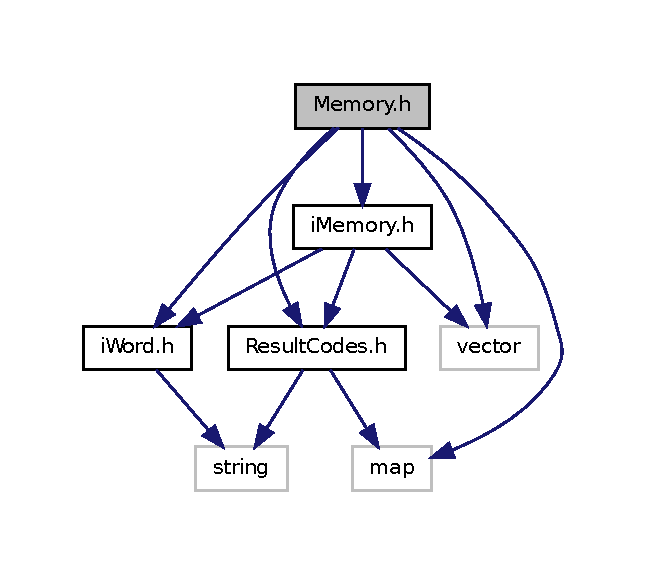
\includegraphics[width=310pt]{Memory_8h__incl}
\end{center}
\end{figure}
\subsection*{Classes}
\begin{DoxyCompactItemize}
\item 
class \hyperlink{classMemory}{Memory}
\begin{DoxyCompactList}\small\item\em Implements \hyperlink{classiMemory}{iMemory}. \item\end{DoxyCompactList}\end{DoxyCompactItemize}


\subsection{Detailed Description}
Definition of private data for the \char`\"{}Memory\char`\"{} class. \begin{DoxyAuthor}{Author}
Joshua Green 

Andrew Groot 
\end{DoxyAuthor}

\hypertarget{ObjParser_8cpp}{
\section{ObjParser.cpp File Reference}
\label{ObjParser_8cpp}\index{ObjParser.cpp@{ObjParser.cpp}}
}


Implements the declarations in \char`\"{}ObjParser.h\char`\"{}.  


Include dependency graph for ObjParser.cpp:\nopagebreak
\begin{figure}[H]
\begin{center}
\leavevmode
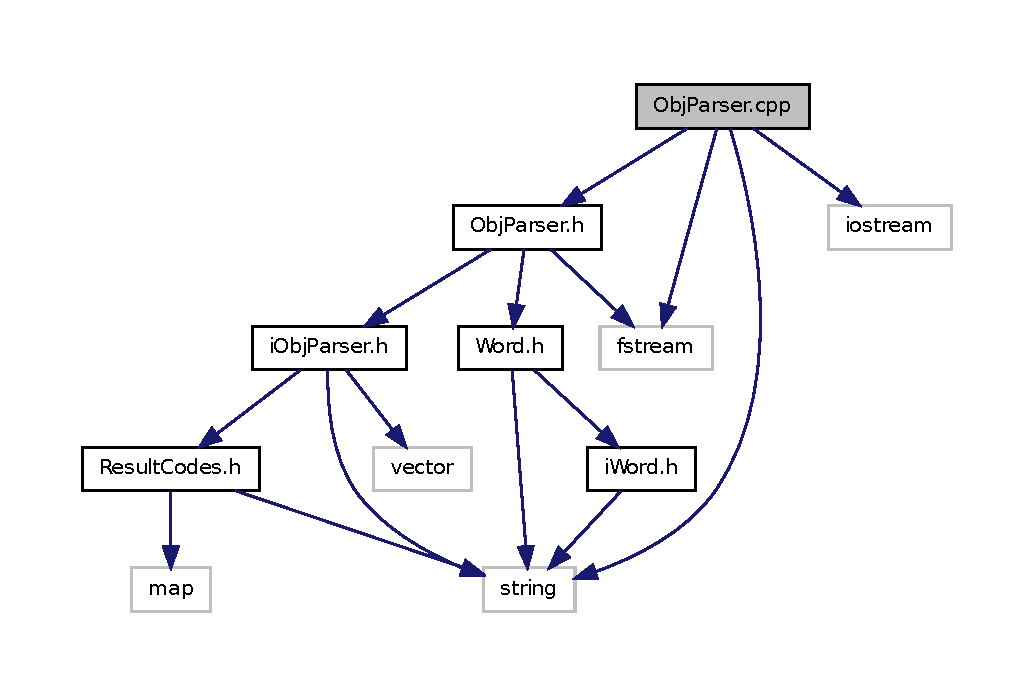
\includegraphics[width=400pt]{ObjParser_8cpp__incl}
\end{center}
\end{figure}


\subsection{Detailed Description}
Implements the declarations in \char`\"{}ObjParser.h\char`\"{}. \begin{DoxyAuthor}{Author}
Ryan Paulson 
\end{DoxyAuthor}

\hypertarget{ObjParser_8h}{
\section{ObjParser.h File Reference}
\label{ObjParser_8h}\index{ObjParser.h@{ObjParser.h}}
}


Definition of private data for the \char`\"{}ObjParser\char`\"{} class.  


Include dependency graph for ObjParser.h:\nopagebreak
\begin{figure}[H]
\begin{center}
\leavevmode
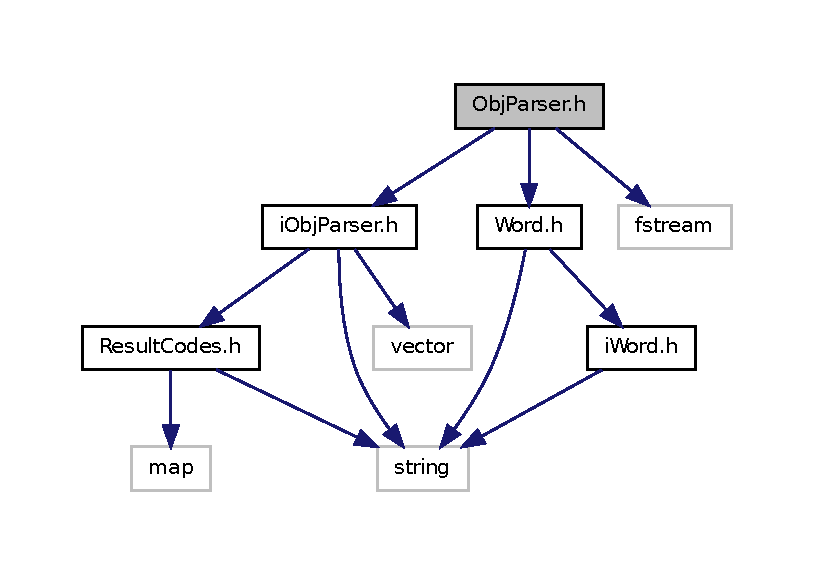
\includegraphics[width=391pt]{ObjParser_8h__incl}
\end{center}
\end{figure}
\subsection*{Classes}
\begin{DoxyCompactItemize}
\item 
class \hyperlink{classObjParser}{ObjParser}
\begin{DoxyCompactList}\small\item\em Implements \hyperlink{classiObjParser}{iObjParser}. \item\end{DoxyCompactList}\end{DoxyCompactItemize}


\subsection{Detailed Description}
Definition of private data for the \char`\"{}ObjParser\char`\"{} class. \begin{DoxyAuthor}{Author}
Ryan Paulson 
\end{DoxyAuthor}

\hypertarget{Register_8h}{
\section{Register.h File Reference}
\label{Register_8h}\index{Register.h@{Register.h}}
}


Definition of private data for the \char`\"{}Register\char`\"{} class.  


Include dependency graph for Register.h:\nopagebreak
\begin{figure}[H]
\begin{center}
\leavevmode
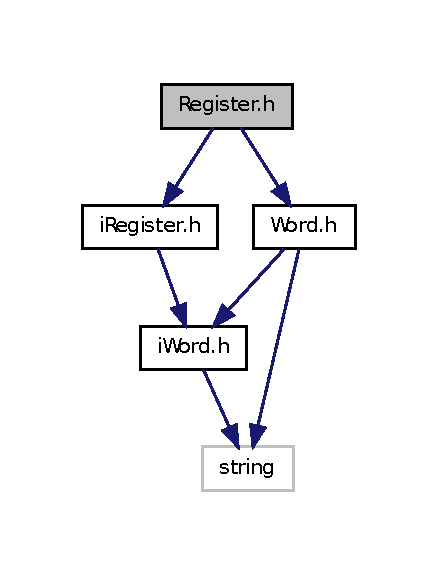
\includegraphics[width=214pt]{Register_8h__incl}
\end{center}
\end{figure}
\subsection*{Classes}
\begin{DoxyCompactItemize}
\item 
class \hyperlink{classRegister}{Register}
\end{DoxyCompactItemize}


\subsection{Detailed Description}
Definition of private data for the \char`\"{}Register\char`\"{} class. \begin{DoxyAuthor}{Author}
Andrew Groot 
\end{DoxyAuthor}

\hypertarget{ResultCodes_8h}{
\section{ResultCodes.h File Reference}
\label{ResultCodes_8h}\index{ResultCodes.h@{ResultCodes.h}}
}


Definition of the Wi-\/11's run-\/time messages.  


Include dependency graph for ResultCodes.h:\nopagebreak
\begin{figure}[H]
\begin{center}
\leavevmode
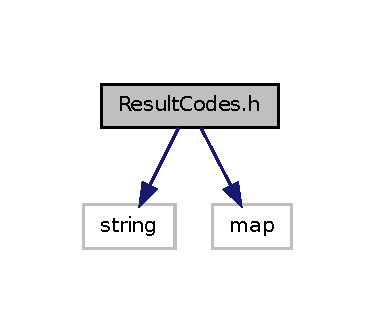
\includegraphics[width=180pt]{ResultCodes_8h__incl}
\end{center}
\end{figure}
\subsection*{Classes}
\begin{DoxyCompactItemize}
\item 
class \hyperlink{classResultDecoder}{ResultDecoder}
\begin{DoxyCompactList}\small\item\em Finds the messages associated with a given result code. \item\end{DoxyCompactList}\end{DoxyCompactItemize}
\subsection*{Namespaces}
\begin{DoxyCompactItemize}
\item 
namespace \hyperlink{namespaceCodes}{Codes}


\begin{DoxyCompactList}\small\item\em Values corresponding to the results of Wi-\/11 function calls. \item\end{DoxyCompactList}

\end{DoxyCompactItemize}
\subsection*{Enumerations}
\begin{DoxyCompactItemize}
\item 
enum {\bfseries RESULT} \{ \par
{\bfseries ERROR\_\-0}, 
{\bfseries SUCCESS}, 
{\bfseries HALT}, 
{\bfseries UNDEFINED}, 
\par
{\bfseries INVALID\_\-HEADER\_\-ENTRY}, 
{\bfseries INVALID\_\-DATA\_\-ENTRY}, 
{\bfseries OUT\_\-OF\_\-BOUNDS}, 
{\bfseries NOT\_\-HEX}, 
\par
{\bfseries FILE\_\-NOT\_\-FOUND}, 
{\bfseries INVALID\_\-TRAP\_\-CODE}
 \}
\end{DoxyCompactItemize}


\subsection{Detailed Description}
Definition of the Wi-\/11's run-\/time messages. \begin{DoxyAuthor}{Author}
Joshua Green 

Andrew Groot 
\end{DoxyAuthor}

\hypertarget{Wi11_8h}{
\section{Wi11.h File Reference}
\label{Wi11_8h}\index{Wi11.h@{Wi11.h}}
}


Definition of the private data for the \char`\"{}Wi11\char`\"{} class.  


Include dependency graph for Wi11.h:\nopagebreak
\begin{figure}[H]
\begin{center}
\leavevmode
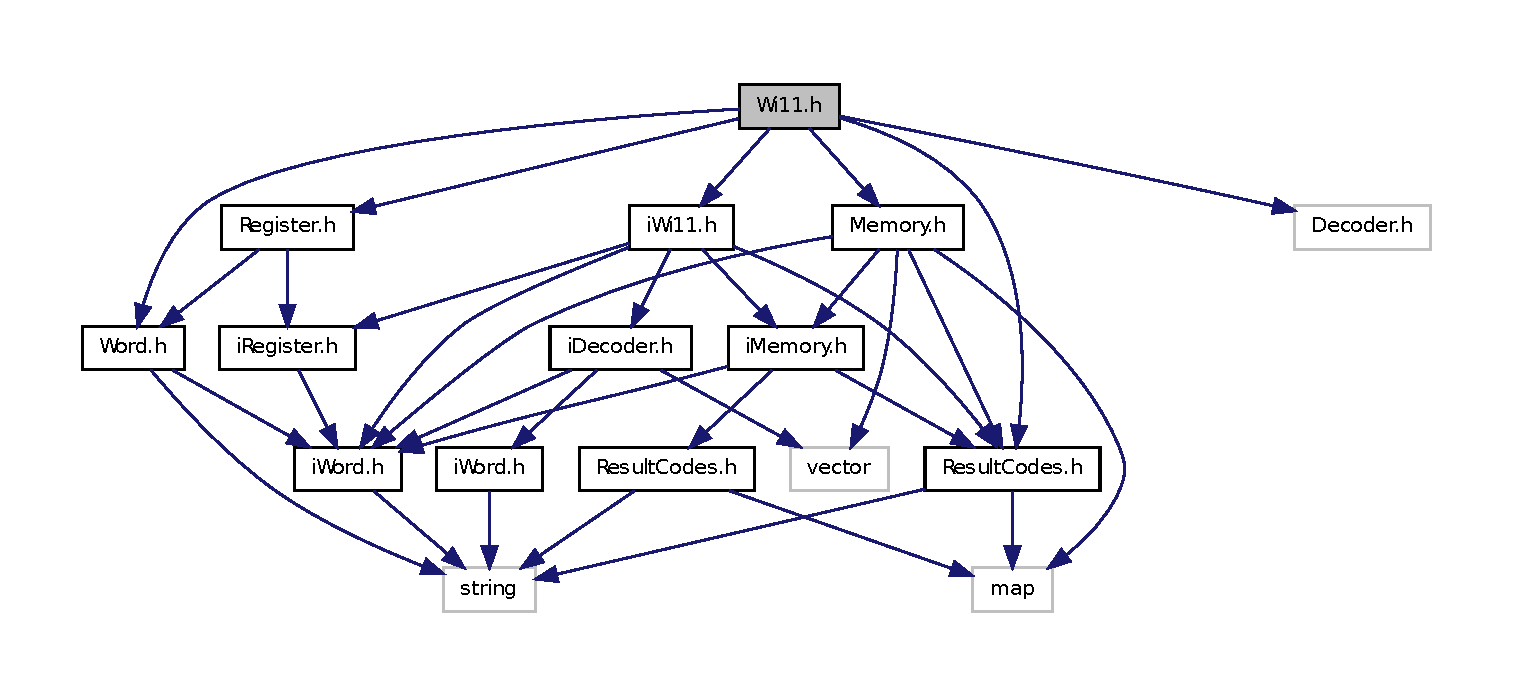
\includegraphics[width=400pt]{Wi11_8h__incl}
\end{center}
\end{figure}
\subsection*{Classes}
\begin{DoxyCompactItemize}
\item 
class \hyperlink{classWi11}{Wi11}
\end{DoxyCompactItemize}


\subsection{Detailed Description}
Definition of the private data for the \char`\"{}Wi11\char`\"{} class. \begin{DoxyAuthor}{Author}
Andrew Groot 
\end{DoxyAuthor}

\hypertarget{Word_8cpp}{
\section{Word.cpp File Reference}
\label{Word_8cpp}\index{Word.cpp@{Word.cpp}}
}


Implements the delcarations in \char`\"{}Word.h\char`\"{}.  


Include dependency graph for Word.cpp:\nopagebreak
\begin{figure}[H]
\begin{center}
\leavevmode
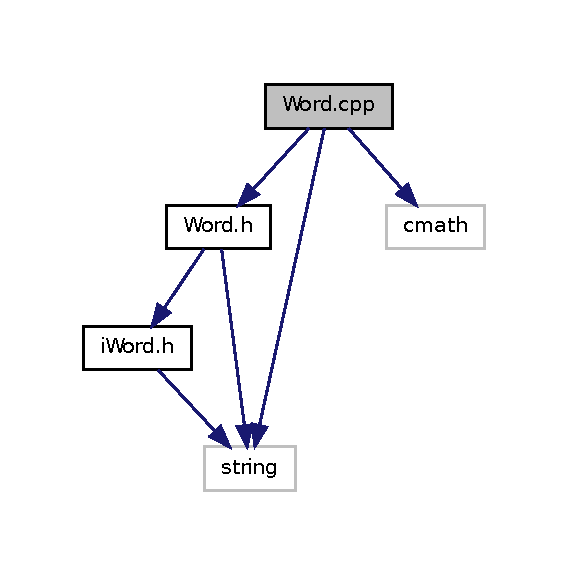
\includegraphics[width=272pt]{Word_8cpp__incl}
\end{center}
\end{figure}


\subsection{Detailed Description}
Implements the delcarations in \char`\"{}Word.h\char`\"{}. \begin{DoxyAuthor}{Author}
Joshua Green 

Andrew Groot 
\end{DoxyAuthor}

\hypertarget{Word_8h}{
\section{Word.h File Reference}
\label{Word_8h}\index{Word.h@{Word.h}}
}


Definition of private data for the \char`\"{}Word\char`\"{} class.  


Include dependency graph for Word.h:\nopagebreak
\begin{figure}[H]
\begin{center}
\leavevmode
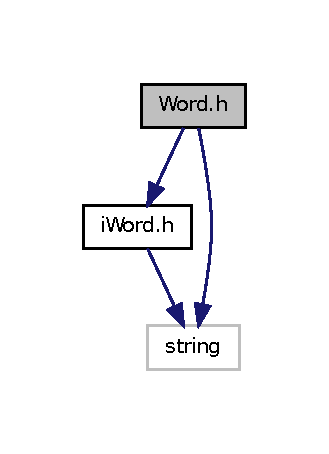
\includegraphics[width=158pt]{Word_8h__incl}
\end{center}
\end{figure}
This graph shows which files directly or indirectly include this file:\nopagebreak
\begin{figure}[H]
\begin{center}
\leavevmode
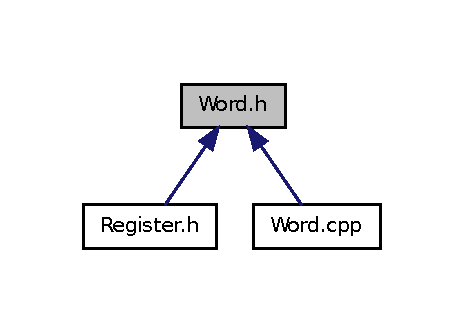
\includegraphics[width=222pt]{Word_8h__dep__incl}
\end{center}
\end{figure}
\subsection*{Classes}
\begin{DoxyCompactItemize}
\item 
class \hyperlink{classWord}{Word}
\end{DoxyCompactItemize}
\subsection*{Defines}
\begin{DoxyCompactItemize}
\item 
\hypertarget{Word_8h_a92ed8507d1cd2331ad09275c5c4c1c89}{
\#define {\bfseries WORD\_\-SIZE}~16}
\label{Word_8h_a92ed8507d1cd2331ad09275c5c4c1c89}

\end{DoxyCompactItemize}


\subsection{Detailed Description}
Definition of private data for the \char`\"{}Word\char`\"{} class. \begin{DoxyAuthor}{Author}
Joshua Green 

Andrew Groot 
\end{DoxyAuthor}

\printindex
\end{document}
